
% ------------------ DOCUMENT SETUP ------------------ 
% The document class defines the document type (report) and sets the font size (10pt)
\documentclass{report}
\author{James Chapman}

% Inputs the Document Packages
% ------------------ PACKAGES ------------------ 

% Packages add extra commands and features to your LaTeX document. 
% Here are some of the most common packages for a thesis document.

% Floating environments for figures and tables
\usepackage{float}

% Color support
\usepackage{color}

% Epigraphs
\usepackage{epigraph}

% Color support for tables
\usepackage[table,xcdraw]{xcolor}

% Mathematical typesetting
\usepackage{amsthm}

% Theorem environments
\newtheorem{corollary}{Corollary}[section]
\newtheorem{definition}{Definition}[section]
\newtheorem{theorem}{Theorem}[section]
\newtheorem{lemma}{Lemma}[section]
\newtheorem{proposition}{Proposition}[section]
\newtheorem{example}{Example}[section]

% Remark environment
\theoremstyle{remark}
\newtheorem{remark}{Remark}

% Restatable theorems
\usepackage{thmtools}
\usepackage{thm-restate}
\declaretheorem[name=Proposition,numberwithin=section]{proprep}
\newtheorem{thm}{Theorem}

% Algorithms
\usepackage[ruled,vlined]{algorithm2e}
\usepackage{algorithmic}

% Vector arrows
\usepackage{esvect}

% TikZ for diagrams
\usepackage{tikz}
\usetikzlibrary{patterns, bayesnet, arrows, backgrounds}

% Hyperlinks
\usepackage{hyperref}
\hypersetup{
    citecolor = blue
}

% Multi-row tables
\usepackage{multirow}

% Appendices
\usepackage[toc,page]{appendix}

% Captioning figures and tables
\usepackage[format=hang,font=normalsize,labelfont=bf,labelsep=colon,singlelinecheck=off, justification=centering]{caption}
\usepackage{subcaption}

% Long tables
\usepackage{longtable}

% Glossaries and acronyms
\usepackage[acronym]{glossaries}

% Font settings
\usepackage[scaled]{helvet}
\usepackage[T1]{fontenc}
\renewcommand\familydefault{\sfdefault}

% Input encoding
\usepackage[utf8]{inputenc}

% Empty pages
\usepackage{emptypage}

% Importing files
\usepackage{import}

% Table of Contents customization
\usepackage{tocloft}

% Title customization
\usepackage{titlesec}

% Table of Contents title customization
\usepackage{titletoc}

% Alternative implementations for LaTeX commands
\usepackage{etoolbox}

% Header and footer control
\usepackage{fancyhdr} 

% Typography enhancements
\usepackage{microtype}

% PDF bookmarks
\usepackage{bookmark}

% Units and symbols
\usepackage{gensymb}
\usepackage{textcomp}

% Bibliography
\usepackage[natbib,style=authoryear,natbib=true]{biblatex}
\addbibresource{publications.bib} % Add the .bib file that contains the references
\addbibresource{References.bib} % Add the .bib file that contains the references

% Sample text
\usepackage{blindtext}

% Tables
\usepackage{booktabs}

% Code listings
\usepackage{listings}
\usepackage{minted}

% Math symbols
\usepackage{amsmath,amsfonts,bm}
\usepackage{amssymb}

% Clever referencing
\usepackage[capitalize,noabbrev]{cleveref}

% Graphics
\usepackage{graphicx}
\usepackage{svg}

% Restating theorems
\usepackage{thm-restate}

% Line spacing control
\usepackage{setspace}

% Mini table of contents
\usepackage{minitoc} 

% Mini TOC font settings
\renewcommand{\mtifont}{\large\sffamily}
\renewcommand{\mtcfont}{\small\sffamily}
\renewcommand{\mtcSfont}{\small\sffamily}
\renewcommand{\mtcSSfont}{\small\sffamily}
\renewcommand{\mtcSSSfont}{\small\sffamily}

% Add to table of contents
\newcommand\addtotoc[1]{
  \refstepcounter{dummy}
  \addcontentsline{toc}{chapter}{#1}
}


% Controls how many subsections the document can take
%  and how many of those will get put into the contents pages.
\setcounter{secnumdepth}{2}
\setcounter{tocdepth}{2}

% Places a dot after Chapter/Section/Subsection number in Table of Contents
\renewcommand{\cftchapaftersnum}{.}
\renewcommand{\cftsecaftersnum}{.}
\renewcommand{\cftsubsecaftersnum}{.}

%  Customize Dot spacing in Table of Contents/List of Figures/Tables
\renewcommand{\cftdotsep}{0.3}

% Numeration Type for Chapters and Sections (Roman I, II, II / Arabic 1, 2, 3)
\renewcommand\thechapter{\Roman{chapter}}
\renewcommand\thesection{\arabic{section}}

% Formatting Table of Contents/Lists titles
\renewcommand{\contentsname}{\normalfont\bfseries\LARGE{CONTENTS}}
\renewcommand{\listfigurename}{\normalfont\bfseries\LARGE{LIST OF FIGURES}}
\renewcommand{\listtablename}{\normalfont\bfseries\LARGE{LIST OF TABLES}}


% Title Formatting customization
\titleformat{\chapter}{\normalfont\bfseries\LARGE}{\thechapter.}{1em}{\MakeUppercase}

\titleformat{\section}{\normalfont\bfseries\large}{\thesection.}{1em}{\MakeUppercase}
\titlespacing*{\section} {0pt} {15pt} {15pt} % left, before, after

\titleformat{\subsection}{\normalfont\bfseries\large}{\thesubsection.}{1em}{}
\titlespacing*{\subsection} {0pt} {10pt} {10pt}

\titleformat{\subsubsection}{\normalfont\bfseries\large}{}{1em}{}
\titlespacing*{\subsubsection} {0pt} {10pt} {10pt}


% HEADER AND FOOTER
\pagestyle{fancy}  % Set Page Style (Header and Footer Style)
\fancyhf{}  % Clears the header and footer (from the default info)

% Header
\renewcommand{\headrulewidth}{0pt}  % Removes the default Horizontal Line in Header
\fancyhead[L]{James Chapman}
\fancyhead[R]{January 2022}

% Footer
\fancyfoot[C]{\thepage} % Page Number

% Change figure numbering per section
\numberwithin{figure}{chapter}
\numberwithin{table}{section}






%  -------------------------------------------------
%  --------- The document starts from here --------- 
%  -------------------------------------------------

\begin{document}

% ------------------  TITLE PAGE -------------------
\begin{titlepage}
\begin{center}
    % Title
    {\LARGE\textbf{Towards Scalable, Flexible, and Interpretable Self-Supervised Learning from Multiview Biomedical Data}
\author{James Chapman\\
    % Subtitle
    \\}}

    \vspace{0.8cm}
    by\\
    \vspace{0.8cm}

    % Author
    {\LARGE\textbf{James Chapman\\}}
    % Date
    \vspace{1.5cm}
    {\LARGE\textbf{January 2022}}

    \vfill

    \textbf{\setstretch{2.0}       
    Upgrade Report\\
    \vspace{1cm}
    i4health CDT\\
    University College London\\}

    \vspace{2cm}
\end{center}
\end{titlepage}


% ----------------------  ABSTRACT -----------------------
\newpage
\chapter*{Abstract} % the Asterix (*) indicates that this section will be added to the table of contents but no number will be present beside it.
% \addcontentsline{toc}{chapter}{Abstract}

Biomedical data are essential for advancing our knowledge and practice of medicine and healthcare. However, biomedical data are also challenging to analyze due to their complexity, heterogeneity, high-dimensionality, and scarcity of labels. To overcome these challenges, self-supervised learning (SSL) has emerged as a promising paradigm for learning from unlabeled data by leveraging inherent structures or patterns in the data. SSL methods can exploit different forms of supervision signals derived from the data itself, such as contrastive learning, reconstruction, prediction, or clustering. SSL methods can also benefit from deep neural networks that can learn expressive and flexible representations from complex and high-dimensional data.

In this thesis, we focus on a specific type of SSL problem, namely multiview SSL, where data are represented by multiple distinct feature groups or modalities that describe the same phenomenon or entity. Each feature group or modality is referred to as a view, and different views may provide complementary or redundant information. Multiview SSL aims to learn useful representations from multiview data by exploiting the inherent structures or patterns across views. Multiview SSL has a wide range of applications in biomedical domains, such as integrating multiple types of genomic data for disease diagnosis or prognosis, generating natural language descriptions from brain images, and understanding human behaviors during social interactions based on multimodal signals.

In this thesis, we propose novel approaches to multiview SSL that are scalable, flexible, and interpretable. We address the following research questions:How can we reformulate classical subspace learning methods as unconstrained optimization problems that can be solved by gradient descent? How can we extend classical subspace learning methods to nonlinear functions using deep neural networks? How can we incorporate different forms of regularization or prior knowledge into subspace learning methods to improve their quality or robustness?

To answer these questions, we develop novel methods for multiview subspace learning that leverage mathematical optimization techniques, deep neural networks, regularization techniques. We evaluate our methods on various real-world biomedical datasets and demonstrate their effectiveness and advantages over existing methods.

% ----------------------  IMPACT STATEMENT -----------------------
\newpage
\chapter*{Impact Statement} % the Asterix (*) indicates that this section will be added to the table of contents but no number will be present beside it.
% \addcontentsline{toc}{chapter}{Impact}

This thesis contributes to the advancement of machine learning and biomedical data analysis by developing novel methods for multiview self-supervised learning that are scalable, flexible, and interpretable. The proposed methods can help researchers and practitioners to analyze complex and high-dimensional biomedical data more efficiently and effectively, and to discover new insights and opportunities for improving health outcomes. The proposed methods can also be applied to other domains where multiview data are available or desirable, such as natural language processing, computer vision, multimedia analysis, and social network analysis. This thesis also provides a valuable reference for future research on multiview self-supervised learning and related topics.

% -----------------  ACKNOWLEDGEMENTS  -------------------
\newpage
\chapter*{Acknowledgements}

Thanks to my supervisors, Professor Janaina Mourao-Miranda and Professor John Shawe-Taylor, for their contributions. 
I am very grateful to the EPSRC UCL Centre for Doctoral Training (CDT) in Intelligent, Integrated Imaging in Healthcare (i4Health) and NIHR UCLH Biomedical
Research Centre for funding this research.
Thanks to G-Research for funding my trip to NeurIPS 2023 to present my work.

To my incredible friends and coauthors, Ana and Lennie, I couldn't have done this without you. Ana, you kept our paper alive when I had given up on it (as well as the PhD). Lennie, your brutal honesty about the work being rubbish made it infinitely better. Florence, I was honored to be included on Fusili and for the hard lessons you taught me in marketing.

To members of the Machine Learning for Neuroimaging group at UCL, the Centre for Medical Imaging Computing, and all of the friends from 90 High Holborn.
Cemre, we could and should have done so much more together, but I am grateful for your advice before you left. 
Agoston, I was inspired your immense knowledge of the field.
Rick, you were everpresent in the office whenever the pandemic allowed, and I am grateful for your advice.
To the Mojo Dojo Casa House, thank you for making my NeurIPS 2023 experience unforgettable.

To the boat clubs of University College London, University of London, and Vesta Rowing Club who have provided an outlet that gave me a sense of progress, purpose, and community, even when academia had me down. Thanks also to all of the friends from the $\frac{1}{2}$ pint club, M\&G, and otherwise who have listened to me complain about my PhD.

Thanks to my mum and dad, obviously this has been a bit of a rollercoaster, but I am grateful for every helpful conversation we have had. And finally with love to Rebecca. On about our third date, you came to visit Leamington Spa to scout out PhDs. You have experienced every good and bad moment. You have been proud of me. We got through this together and we will get through the next thing together too.




% -------------------  LIST OF Publication ---------------------
\newpage
\chapter*{Publications}
\label{Publications}




% -------------------  LIST OF FIGURES --------------------
\newpage 
% {\let\oldnumberline\numberline       % Uncomment to add the word 'Figure' to figure number in List of Figures
%\renewcommand{\numberline}{\figurename~\oldnumberline}  
\listoffigures%
% \addcontentsline{toc}{chapter}{List of Figures} % Add List of figures into contents without any numeration 

% -------------------  LIST OF TABLES ---------------------
\newpage
\listoftables 
% \addcontentsline{toc}{chapter}{List of Tables} % Add List of tables into contents without any numeration 

% -------------------  ACRONYMS ---------------------
\newpage

% -------------------  NOTATION ---------------------
\newpage


% ------------------  TABLE OF CONTENTS --------------------
\tableofcontents 


%\textbf{Keywords:} Machine Learning, Neuroimaging, Canonical Correlation Analysis



% ------------------  CHAPTER START  --------------------
\graphicspath{{chapters/introduction/}}
\chapter{Introduction}\label{chap:introduction}

 \epigraph{All models are wrong, some are useful.}{\textit{G. Box}}

In an era marked by an overwhelming abundance of data, the ability to distill wisdom from information becomes not just a skill but a necessity.
This thesis addresses the critical gap between the immense volumes of biomedical data available and our current capacity to synthesize this data into actionable insights for healthcare.

\section{Setting the Stage: The Challenge of Big Data in Biomedical Research}

The advent of advanced technologies in biomedical research has led to a deluge of data.
From genomic sequences to patient health records, this data holds the key to unlocking mysteries of human health and disease.
However, the challenge lies not in data collection but in its analysis and interpretation – in turning this vast information into wisdom.

\textbf{This thesis presents innovative methodologies for scaling multimodal data fusion to massive datasets}, aiming to transform the way biomedical data is analyzed and understood.
By leveraging advancements in self-supervised learning and data integration techniques, it seeks to bridge the gap between data abundance and knowledge creation.

\section{Thesis Structure and Contributions}

This thesis offers three primary contributions:

\begin{itemize}
    \item Developing a regularization method for CCA using structured priors, including the Elastic Net, to improve interpretability.
    \item Proposing the use of loadings over weights in CCA for better interpretability and relevance to biomedical data generation processes.
    \item Creating a new gradient descent-based formulation for CCA and generalized eigenvalue problems, suitable for large datasets.
\end{itemize}

\subsection{Chapter Summaries}

\textbf{Chapter \ref{chap:background}} reviews multiview and self-supervised learning techniques, focusing on their application in biomedical data.

\textbf{Chapter \ref{chap:als}} introduces a method to regularize CCA using structured priors, demonstrated with Human Connectome Project and Alzheimer's Disease Neuroimaging Initiative data.

\textbf{Chapter \ref{chap:loadings}} examines the relationship between loadings and weights in CCA, using simulated data to show the advantages of loadings for interpretability.

\textbf{Chapter \ref{chap:gradient_descent}} presents a new loss function for generalized eigenvalue problems, applicable to CCA and SSL methods, and demonstrates its effectiveness with various benchmarks.

\textbf{Chapter \ref{chap:software}} introduces CCA-Zoo, a Python package implementing the methodologies of this thesis, and discusses its role in the Python ecosystem and biomedical research.

\textbf{Chapter 7} discusses the implications, challenges, and future directions for the research presented in this thesis.

This thesis aims to address the gap between the potential of biomedical data and the capabilities of current analytical methods.


\graphicspath{{chapters/background/}}


\chapter{Background: Multiview Machine Learning: Concepts, Methods, and Limitations}\label{ch:background}
 \epigraph{Principal Component Analysis is a dimensionally invalid method that gives people a delusion that they are doing something useful with their data. If you change the units that one of the variables is measured in, it will change all the “principal components”! It’s for that reason that I made no mention of PCA in my book.}{Professor David MacKay}
\minitoc

\section{Introduction}

This chapter provides the foundational knowledge needed to understand the thesis as a whole, while the individual chapters will provide more specific background information as needed.

\section{Machine Learning and Multiview Learning}

Machine learning encompasses methods that enable models to learn patterns and make decisions from data.
Machine learning methods are typically categorised by a training set of data, which is used to learn a model, and a test set of data, which is used to evaluate the model.
Arguably the most common machine learning paradigm is supervised learning, where the training data consists of pairs of inputs and outputs, and the model learns to predict a function which maps the inputs to the outputs.
This function is then used to predict the outputs for new inputs.
The goal of supervised learning is to learn a function that generalizes well to new data, i.e. to make accurate predictions on unseen data.
Unsupervised and self-supervised learning are common machine learning paradigms where the training data consists of inputs only, and the model learns to find patterns in the data.
While the distinction between the two is somtimes blurred, unsupervised learning has been used to describe dimensionality reduction, clustering, and generative modelling algorithms.
Self-supervised learning (SSL) has been used to describe a special case of unsupervised learning, where labels are generated from the data itself, rather than being provided by an external source.
SSL  is a paradigm where the training signal is derived from the data itself, rather than relying on external labels \citep{balestriero2023cookbook}.
The cornerstone of SSL is the concept of a `pretext task', a learning task created from the data that trains the model to capture useful features or representations.
Most famously, SSL is the backbone to the success of Large Language Models \citep{vaswani2017attention} and in particular ChatGPT \citep{chatgpt}, a language model trained on a pretext task of predicting masked words in a sentence.
SSL methods have also recently been shown to outperform supervised methods for certain computer vision tasks for large datasets \citep{goyal2019scaling}.


\subsection{Multiview Machine Learning}
This thesis is focussed on multiview machine learning.
Here, data from different sources or modalities, referred to as \gls{views}, such as neuroimaging, genomics, and clinical records, are analyzed collectively to unveil underlying patterns.
Multiview machine learning encompasses a variety of techniques aimed at learning from data that have multiple sources or modalities, also known as \gls{views}.
These techniques can also be broadly classified into supervised and self-supervised multiview learning, with some algorithms straddling the boundary between the two.

\subsubsection{Supervised Multiview Learning}

In supervised multiview learning, the goal is to integrate information from multiple distinct views or feature sets to improve the predictive performance of a model. This approach often involves using one view as the target, with other views serving as inputs. For instance, in the context of mental health, we can consider behavioural data as a dependent variable influenced by multiple independent variables like brain activity and demographics. Figure \ref{fig:mentalhealthsupervised} illustrates this concept, where behavioural patterns ($y_1$) are predicted based on features from brain activity ($x_1$) and demographic information ($x_2$).

\begin{figure}
    \centering
    \tikz{
    % nodes
        \node[obs, minimum size=3cm, align=center] (y1) {Behaviour\\$y_1$}; % Behaviour node as y1
        \node[obs, left=of y1, minimum size=3cm, align=center] (x1) {Brain\\$x_1$}; % Brain node as x1
        \node[obs, below=of x1, minimum size=3cm, align=center] (x2) {Demographics\\$x_2$};
        \edge{x1} {y1}
        \edge{x2} {y1}}
        \caption[Independent and Dependent Variable Model of Mental Health]{\textit{\textbf{Independent and Dependent Variable Model of Mental Health:}} From this perspective, behavioural data is considered to be dependent on brain activity and demographics}\label{fig:mentalhealthsupervised}
\end{figure}

Multiple Kernel Learning (MKL) \citep{gonen2011multiple} is a prominent example of supervised multiview learning, where the algorithm learns to combine kernel representations of the different views.
This enhances the model's predictive capabilities compared to using a single kernel.
With the advent of deep learning, the underlying concept of MKL has been extended to deep learning architectures.
These architectures enable the model to learn and combine representations from various views more effectively \citep{guo2019deep}.
I contributed to this line of research through the software package Fusili \citep{florence_townend_2023_10228564}, which implements a number of deep-learning based multi-modal data fusion methods for supervised learning.

\subsubsection{Self-Supervised Multiview Learning}

In contrast to supervised multiview learning, where explicit labels guide the learning process, self-supervised multiview learning operates under the hypothesis that different views are manifestations of a shared, yet hidden, latent variable \citep{zong2023self}.
This approach, as evidenced in the latent variable model of mental health illustrated in Figure \ref{fig:mentalhealthselfsupervised}, suggests that both neuroimaging and behavioural data are influenced by an underlying factor, such as the severity of a mental health condition, which remains unobserved.

\begin{figure}
    \centering
    \tikz{
    % nodes
        \node[latent, align=center, minimum size=2cm] (Z) {Severity\\z};
        %
        \node[obs, below left=of Z, minimum size=2cm, align=center] (x1) {Brain\\$x^{(1)}$};
        \node[obs, below right=of Z, minimum size=2cm, align=center] (x2) {Behaviour\\$x^{(2)}$};
        % edges
        \edge{Z} {x1}
        \edge{Z} {x2}}
    \caption[Latent Variable Model of Mental Health]{\textit{\textbf{Latent Variable Model of Mental Health:}} From this perspective the neuroimaging modality and behavioural data are both considered to have been generated with distributions conditioned on the severity of a mental health condition}\label{fig:mentalhealthselfsupervised}
\end{figure}

A key challenge in self-supervised learning is designing pretext tasks to infer this latent source from the available views.
A common approach is to estimate a common low-dimensional representation of the variance in the data from both \gls{views}.
In most objectives of this form, this ammounts to identifying the mutual information between the \gls{views}.
These representations may be informative for their own sake, identifying common factors between the \gls{views}, or they may be used as inputs to a downstream task, such as classification or regression.

\subsection{Conditional Independence, Causality, and Multiview Learning}

The graphical model in Figure \ref{fig:mentalhealthsupervised} represents the assumption that the brain and demographics are independent variables, and that the behaviour is a conditional variable, dependent on both the brain and demographics.

On the other hand, the graphical model in Figure \ref{fig:mentalhealthselfsupervised} represents the assumption that the brain and behaviour are conditionally independent given the severity of an unobserved `latent' mental health condition.

\citet{reichenbach1956direction} introduced the epoynmous Reichenbach's principle, which states that if two variables are correlated, then either one causes the other, or both are caused by a third variable.
While the relationship between conditional independence and causality is nuanced \citep{pearl2009causality}, it is clear that our assumptions about the causal structure of the data can inform our choice of multiview learning algorithm.
In particular, we could envision a number of causal structures that could give rise to the observed data in Figure \ref{fig:mentalhealthselfsupervised}:

\begin{itemize}
    \item direct causation (brain influencing behavior or vice versa or even both)
    \item both being influenced by a common, possibly unobserved, cause
    \item no direct causal link between them
\end{itemize}

In the first case, we might be more inclined to use a supervised multiview learning algorithm to predict one view from the other.
In the second case, we might be more inclined to use a self-supervised multiview learning algorithm to estimate the latent variable.

\subsubsection{Complementary and Redundant Information}
The nature of the information provided by different \gls{views} (such as neuroimaging and behavioral data) is important for understanding multiview learning models.
A particularly useful distinction is between complementary and redundant information \citep{nguyen2020multiview,lyu2021understanding, chen2022representation}.
The complementary information in views offers unique insights into different aspects of the same subject. For instance, in mental health studies, neuroimaging might reveal structural changes in the brain that are not (yet) present in presented behavioural phenotypes, while behavioral data could be influenced by demographic factors that do not present as structural differences in the brain. Both these views together provide a more holistic understanding of a mental health condition.
Conversely, redundant information in different views refers to overlapping or similar data presented from various angles. For instance, a specific mental health condition may manifest in both observable behavioral changes and detectable neuroimaging markers. While each view alone could suggest the presence of the condition, their combination, due to redundancy, can enhance the reliability of the diagnosis. This redundancy is not merely repetitive; it plays a crucial role in denoising and validating findings. In essence, if both neuroimaging and behavioral data independently point to the same diagnosis, the confidence in this diagnosis increases.
The `Wisdom of Crowds' phenomenon, where the collective average of multiple estimates tends to be more accurate than individual estimates, exemplifies the strength of redundant information \citep{galton1907vox}, as illustrated in Figure \ref{fig:wisdomofcrowds}. This principle is akin to the redundancy in multiview data, where multiple views converge to a more accurate or robust conclusion than any single view alone.

\begin{figure}
    \centering
    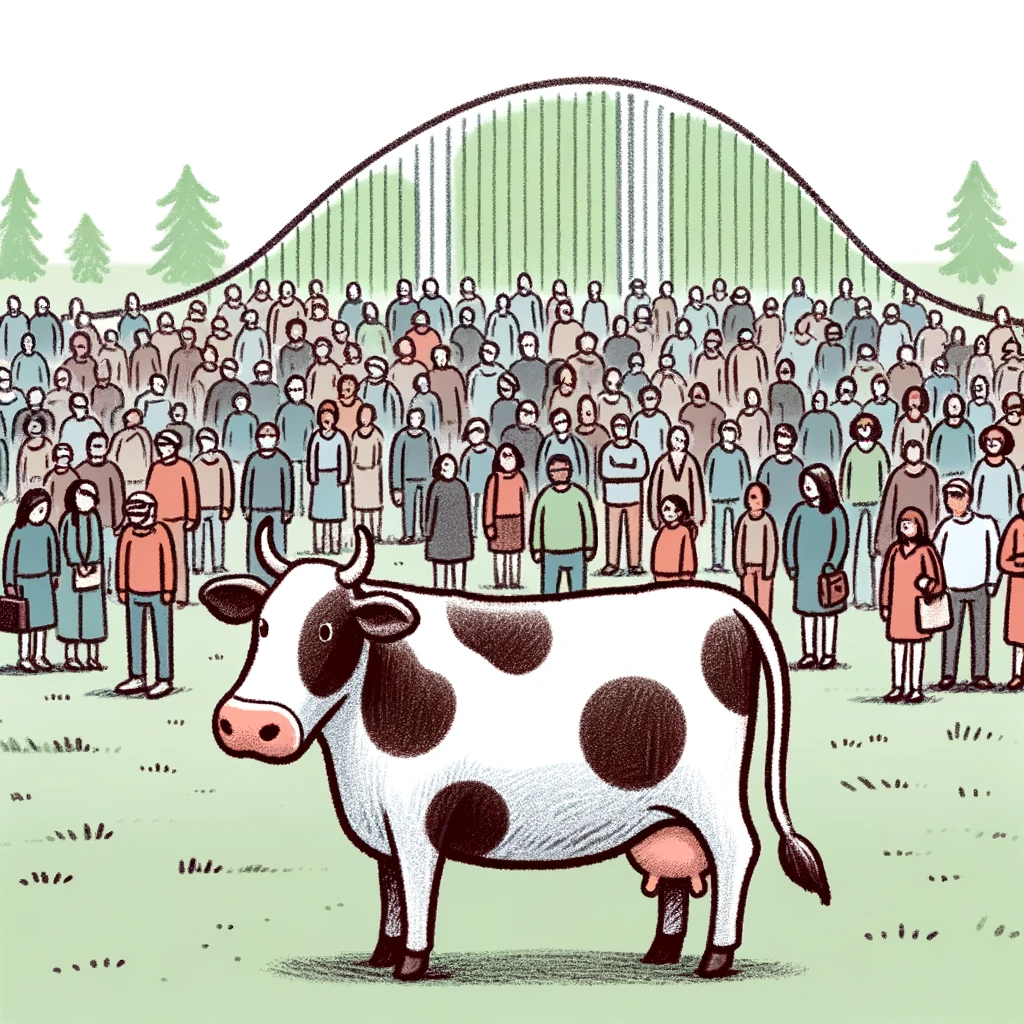
\includegraphics[width=0.5\textwidth]{figures/cow.png}
    \caption[The Wisdom of Crowds]{\textit{\textbf{The Wisdom of Crowds:}} The average of multiple noisy estimates of the weight of a cow is more accurate than any individual estimate. Created with the assistance of DALL·E 2}\label{fig:wisdomofcrowds}
\end{figure}

In this thesis, we will explore Canonical Correlation Analysis, a multiview learning method predicated on the assumption that different \gls{views} provide complementary information about latent variables. The following sections will establish a formal framework for representation learning and motivate the use of Canonical Correlation Analysis in harnessing complementary information from multiview data.

\section{Learning Representations: Definitions and Notation}

Suppose we have a sequence of vector-valued random variables $X\sps{i} \in \R^{D_i}$ for $i \in \{1, \dots, I \}$
We want to learn meaningful $K$-dimensional representations
\begin{equation}
    \label{eq:general-form-of-representations}
    Z\sps{i} = f\sps{i}( X\sps{i}; \theta\sps{i}).
\end{equation}
For convenience, define $D = \sum_{i=1}^I D_i$ and $\theta = \left(\theta\sps{i}\right)_{i=1}^I$.
Without loss of generality take $D_1 \geq D_2 \geq \cdots \geq D_I$.
We will consistently use the subscripts $i,j \in [I]$ for \gls{views};
$d \in [D_i]$ for dimensions of input variables;
and $l,k \in [K]$ for dimensions of representations - i.e. to subscript dimensions of $Z\sps{i}, f\sps{i}$.
Later on we will introduce total number of samples $N$.

In this report, when the functions $f$ are linear, we will typically refer to $u_k$ as \gls{weights}, $Z_k = X_k u_k$ as \gls{representations} or \gls{latent variables} (noting that in the CCA literature they are sometimes referred to as canonical variables \citep{borga_learning_1998}), depending on the context.
We will sometimes consider a matrix $U = \left(u_1, \dots, u_K\right) \in \R^{D \times K}$ of \gls{weights}, and a matrix $Z = \left(Z_1, \dots, Z_K\right) \in \R^{N \times K}$ of representations.
We will refer to the Pearson correlation between features and their respective latent variable $\Corr(X\sps{i}_j, Z_k)$ as the \gls{loadings} of $X\sps{i}_j$ on $Z_k$ \citep{rosipal2005overview, alpert1972interpretation, borga_learning_1998}, noting that the same concept has also been referred to as structure correlations \citep{meredith1964canonical}.

%Covariance matrices
We will use the notation $\Sigma_{ij}=\Cov(X\sps{i}, X\sps{j})$ for the population covariance matrix between the random variables associated with view $i$ and $j$. We will also use $\Sigma_{ii}= \Cov(X\sps{i})$ for the population covariance matrix of the random variables associated with view $i$ with each other.

\subsection{Generalized Eigenvalue Problems in linear algebra}
A Generalized Eigenvalue Problem (GEP) is defined by two symmetric matrices $A,B\in \mathbb{R}^{D\times D}$ \citep{stewart_matrix_1990}\footnote{more generally, $A,B$ can be Hermitian, but we are only interested in the real case}.
They are usually characterized by the set of solutions to the equation:
\begin{align}
    \label{eq:igep}
    Au=\lambda Bu
\end{align}
with $\lambda \in \R, u \in \R^D$, called (generalized) eigenvalue and (generalized) eigenvector respectively.
When $B$ is positive definite, then the GEP becomes equivalent to an eigen-decomposition of the symmetric matrix $B^\mhalf A B^\mhalf$ \citep{ghojogh2019eigenvalue}.
In addition, one can find a basis of eigenvectors spanning $\R^D$.
We define a top-$K$ subspace to be one spanned by some set of eigenvectors {$u_1,\dots,u_K$} with the top-$K$ associated eigenvalues $\lambda_1 \geq \dots \geq \lambda_K$.
We say a matrix $U \in \R^{D \times K}$ defines a top-$K$ subspace if its columns span one.

\paragraph{Uniqueness}
In GEPs, the eigenvectors $u$ are not in general unique, but the generalized eigenvalues $1 \geq \lambda_1 \geq \lambda_2 \geq \dots \geq 0$ are unique \citep{mills1988calculation}.

\subsection{Principal Components Analysis}

Principal Components Analysis \citep{hotelling1933analysis} (\acrshort{pca}) is a classical method in unsupervised machine learning for representation learning.
It is widely used for dimensionality reduction and feature extraction.
The primary goal of \acrshort{pca} is to transform the original high-dimensional data into a new coordinate system defined by orthogonal axes, capturing the most relevant aspects of the data.

In \acrshort{pca}, the representations are constrained to be linear transformations of the form:
\begin{equation}
    \label{eq:pca-linear-function-def}
    Z_k = X u_k,
\end{equation}
where $u_k$ are orthonormal basis vectors such that:
\begin{equation}
    \label{eq:pca-orthonormality-constraint}
    u_k^\top u_k = 1, \quad
    u_k^\top u_l = \delta_{kl} \text{ for } k \neq l.
\end{equation}

The primary goal of \acrshort{pca} is to maximize the variance of the representations \(Z_k\), finding the directions of maximal variance in the data.

\subsubsection{Optimization and Solution}
Mathematically, for the first principal component, this can be formulated as:

\begin{align}
    u_{\text{opt}} & = \underset{u}{\text{argmax}} \left( u^\top \Sigma u \right) \\
    \text{subject to:} \notag                                                     \\
    u^\top u       & = 1 \notag
\end{align}

Where \(\Sigma = \mathbb{E}[X^\top X]\) is the population covariance matrix of the single view data $X$.

The Lagrangian for this problem is:
\begin{equation}
    f(u,\lambda) = u^\top \Sigma u + \lambda(1 - u^\top u),
\end{equation}
where \(\lambda\) is the Lagrange multiplier.
Differentiating the Lagrangian yields the first-order conditions:
\begin{align}
    \Sigma u & = \lambda u, \\
    u^\top u & = 1.
\end{align}

\paragraph{Eigenvalue Problem}

This transforms the problem into an eigenvalue equation for the covariance matrix \(\Sigma\), which can be efficiently solved using standard libraries such as scikit-learn \citep{pedregosa2011scikit}.

The first principal component therefore corresponds to the eigenvector associated with the largest eigenvalue \(\lambda\).
Subsequent components are the remaining eigenvectors ordered by their corresponding eigenvalues.

\subsubsection{Limitations}
There are two major limitations of \acrshort{pca} that are relevant to this thesis.
The first is revealed by the epigraph of this chapter, which highlights the fact that \acrshort{pca} is not scale invariant.
This means that the principal components are sensitive to the scale of the data, and therefore the units in which the data is measured.
Furthermore, the interpretation of the principal components is challenging; they are linear combinations of all of the original features. For this reason, sparse variants of \acrshort{pca} have been developed \citep{zou2006sparse,zou2018selective}, which aim to find sparse linear combinations of the original features; interpretable as a subset of the original features contributing to a significant proportion of the variance in the data.
Another major limitation of \acrshort{pca} in the context of multiview learning is that it does not explicitly take advantage of either the redundancy or the complementary information in multiview data, even if we concatenate the views into a single random variable $X$.
Nevertheless, \acrshort{pca} remains a popular tool in practice \citep{greenacre2022principal} and is a useful baseline for multiview learning methods, and we will use it as a point of comparison throughout this thesis.

\subsection{Partial Least Squares}

Partial Least Squares (PLS) \citep{wold1975path} aims to maximize the shared covariance between two paired sets of data, referred to as \gls{views}. \acrshort{pls} can be seen as a generalization of \acrshort{pca}, where \acrshort{pca} becomes a special case when the two \gls{views} are identical.

\acrshort{pls} optimises for the dot product between the two views, a measure of similarity.

\begin{align}
    \label{eq:dot-product}
    \langle X\sps{1}u^{(1)}, X\sps{2}u^{(2)} =\sqrt{u\spsT{1}\Sigma_{11}u\sps{1}} \sqrt{u\spsT{2}\Sigma_{22}u\sps{2}} \cos(\theta)
\end{align}

Where $\theta$ is the angle between the two representations.
In order to constrain the problem, we set the norms of the weights to 1.

\subsubsection{Optimization and Solution}

The constrained optimization problem for \acrshort{pls} can therefore be formulated as:

\begin{align}
    u\sps{1}_{\text{opt}} & = \underset{u\sps{1}}{\mathrm{argmax}} \{ u\spsT{1} \Sigma_{12} u\sps{2} \} \\
    \text{subject to:} \notag                                                                             \\
    u\spsT{1}u\sps{1}   & = 1 \notag                                                                    \\
    u\spsT{2}u\sps{2}   & = 1 \notag
\end{align}

The Lagrangian for this optimization problem can be formulated as:

\begin{equation}
    f(u\sps{1}, \lambda) = u\spsT{1} \Sigma_{12} u\sps{2} + \lambda_1 (1 - u\spsT{1}u\sps{1}) + \lambda_2 (1 - u\spsT{2}u\sps{2})
\end{equation}

Upon deriving the first order conditions, we get:

\begin{align}
    \Sigma_{21} u\sps{1} & = \lambda_2 u\sps{2} \\
    \Sigma_{12} u\sps{2} & = \lambda_1 u\sps{1} \\
    u\spsT{1}u\sps{1}  & = 1                  \\
    u\spsT{2}u\sps{2}  & = 1
\end{align}

By substituting the constraint conditions into these equations, we find that \( \lambda_1 = \lambda_2 = \lambda \) by symmetry. Further simplification yields:

\begin{align}
    \Sigma_{21} \Sigma_{12} u\sps{2} & = \lambda^2 u\sps{2} \\
    \Sigma_{12} \Sigma_{21} u\sps{1} & = \lambda^2 u\sps{1}
\end{align}

\paragraph{Eigenvalue Problem}

Once again, we see that solving these equations will yield the \( u\sps{1} \) and \( u\sps{2} \) vectors as eigenvectors, this time of \( \Sigma_{12} \Sigma_{21} \) and \( \Sigma_{21} \Sigma_{12} \), respectively \citep{hoskuldsson1988pls}.

\paragraph{Generalized Eigenvalue Problem}

We can also represent the system of equations in matrix form as follows:

\begin{align}
    \begin{pmatrix}
        0           & \Sigma_{12} \\
        \Sigma_{21} & 0
    \end{pmatrix}
    \begin{pmatrix}
        u\sps{1} \\
        u\sps{2}
    \end{pmatrix}
    =
    \lambda
    I
    \begin{pmatrix}
        u\sps{1} \\
        u\sps{2}
    \end{pmatrix}
\end{align}

Which is of the form $A v = \lambda B v$. \acrshort{pls} is therefore also defined by the solution to a single generalized eigenvalue problem.

Given the notions of uniqueness in GEPs, the weights $u$ are not in general unique but we can write the vector of generalized eigenvalues $(\lambda_1, \dots, \lambda_K)$ representing covariances as:

\begin{align}
    \label{eq:pls-vector-of-correlations-def}
    \PLS_K(X^{(1)},X^{(2)}) \defeq (\lambda_k)_{k=1}^K
\end{align}

\subsubsection{Limitations} Like \acrshort{pca}, a major problem with applying \acrshort{pls} to neuroimaging and behavioural modalities is that \acrshort{pls} is not scale invariant.
This is because the dot product in equation~\ref{eq:dot-product} is not scale invariant since it is not normalized by the norms of the representations.
Since representations with larger norms will have larger dot products, \acrshort{pls} is biased towards larger representations.
It is therefore also biased towards the largest principal components in the data \citep{helmer2020stability}.
This is particularly problematic when there is a low signal to noise ratio since \acrshort{pls}.
Like \acrshort{pca}, another issue is the lack of sparsity in the \acrshort{pls} solution which has been an active area of research \citep{chun2010sparse, witten2009penalized}.

\subsection{Canonical Correlation Analysis}\label{sec:cca}

In Canonical Correlation Analysis (\acrshort{cca}), we aim to find the directions that maximize correlation, as opposed to maximizing covariance between two \gls{views} of a dataset.
This can be viewed as maximizing the cosine similarity between the two views, rather than the dot product, as in \acrshort{pls}.
Rearranging equation~\ref{eq:dot-product} yields:

\begin{align}
    \label{eq:cosine-similarity}
    \cos(\theta) = \frac{\langle X\sps{1}u^{(1)}, X\sps{2}u^{(2)}}{\sqrt{\langle X\sps{1}u^{(1)}, X\sps{1}u^{(1)}}\cdot \sqrt{\langle X\sps{2}u^{(2)}, X\sps{2}u^{(2)}}}= \frac{u\spsT{1}\Sigma_{12}u\sps{2}}{\sqrt{u\spsT{1}\Sigma_{11}u\sps{1}} \sqrt{u\spsT{2}\Sigma_{22}u\sps{2}}}
\end{align}

and we can see that the dot product from equation~\ref{eq:dot-product} is normalised by the inner products so that \acrshort{cca} is scale invariant, unlike \acrshort{pls}.
All that matters is the angle between the representations, not their magnitude.
Once again, in order to constrain the problem, we this time set the norms of the representations to 1.

\subsubsection{Optimization and Solution}
The optimization problem for \acrshort{cca} can be expressed as:

\begin{align}
    & u_{\text{opt}}=\underset{u}{\mathrm{argmax}}\{ u\spsT{1}X\spsT{1}X\sps{2}u\sps{2} \} \\
    & \text{subject to:} \notag                                                                \\
    & u\spsT{1}\Sigma_{11}u\sps{1}=1 \notag                                                  \\
    & u\spsT{2}\Sigma_{22}u\sps{2}=1 \notag
\end{align}

Although non-convex, numerous methods exist for solving the \acrshort{cca} problem, including eigendecomposition and generalized eigendecomposition solvers \citep{uurtio2017tutorial} and block coordinate descent via alternating least squares regressions \citep{golub1995canonical,sun2008least}.

The first-order conditions derived in the same manner as the \acrshort{pls} case are:

\begin{align}
    \label{CCA:FOCs}
    & \Sigma_{21}u\sps{1}=\lambda\sps{2} \Sigma_{22}u\sps{2} \\
    & \Sigma_{12}u\sps{2}=\lambda\sps{1} \Sigma_{11}u\sps{1} \\
    & u\spsT{1}\Sigma_{11}u\sps{1}=1                       \\
    & u\spsT{2}\Sigma_{22}u\sps{2}=1
\end{align}

\paragraph{Eigenvalue Problems}

Substituting the second two conditions into the first two, we get \(\lambda\sps{1}=\lambda\sps{2}=\lambda\). Finally, substituting the first two conditions into each other, we find the eigenvalue problems:

\begin{align}\label{eq:cca-eigenvalue-problems}
    & \Sigma_{11}^{-1}\Sigma_{12}\Sigma_{22}^{-1}\Sigma_{21}u\sps{1}=\lambda^2u\sps{1} \\
    & \Sigma_{22}^{-1}\Sigma_{21}\Sigma_{11}^{-1}\Sigma_{12}u\sps{2}=\lambda^2u\sps{2}
\end{align}

An alternative form of the \acrshort{cca} problem can be developed by reparameterizing \(u\sps{i*}=\Sigma_{ii}^{-\frac{1}{2}}u\sps{i}\). The optimization problem then becomes:

\begin{align}\label{eq:cca-reparameterized}
    & u_{\text{opt}}=\underset{u}{\mathrm{argmax}}\{ u\spsT{1}\Sigma_{11}^{-\frac{1}{2}}\Sigma_{12}\Sigma_{22}^{-\frac{1}{2}}u\sps{2} \} \\
    & \text{subject to:} \notag                                                                                                            \\
    & u\spsT{1}u\sps{1}=1 \notag                                                                                                         \\
    & u\spsT{2}u\sps{2}=1 \notag
\end{align}

This reparameterized form will later underpin Deep Canonical Correlation Analysis (\acrshort{dcca}) through the matrix $T=\Sigma_{11}^{-\frac{1}{2}}\Sigma_{12}\Sigma_{22}^{-\frac{1}{2}}$.
This form also shows that \acrshort{pls} and \acrshort{cca} can be made equivalent by whitening the data matrices before constructing the covariance matrix.
When the number of features exceeds the number of samples (\(p>n\)), \acrshort{cca} becomes degenerate because the within-view covariance matrices cannot be inverted—contrasting with \acrshort{pls}, which is always computable.

\paragraph{Generalized Eigenvalue Problem}

We can also represent the system of equations in equation~\ref{CCA:FOCs} as a matrix equation:

\begin{align}
    \begin{pmatrix}
        0           & \Sigma_{12} \\
        \Sigma_{21} & 0
    \end{pmatrix}
    \begin{pmatrix}
        u\sps{1} \\
        u\sps{2}
    \end{pmatrix}
    =
    \lambda
    \begin{pmatrix}
        \Sigma_{11} & 0           \\
        0           & \Sigma_{22}
    \end{pmatrix}
    \begin{pmatrix}
        u\sps{1} \\
        u\sps{2}
    \end{pmatrix}
\end{align}

Which is once again of the form $A u = \lambda B u$. \acrshort{cca}, like \acrshort{pls}, is therefore also defined by the solution to a single generalized eigenvalue problem.

\paragraph{Canonical Correlations}
In the case of \acrshort{cca}, the generalized eigenvalues $\lambda$ are generally called canonical correlations \citep{hotelling1935canonical, hotelling1992relations}.
Given the notions of uniqueness in GEPs, the weights $u$ are not in general unique but we can write the vector of generalized eigenvalues or canonical correlations as:
\begin{align}
    \label{eq:cca-vector-of-correlations-def}\small
    \CCA_K(X^{(1)},X^{(2)}) \defeq (\rho_k)_{k=1}^K
\end{align}

\subsubsection{Limitations}

A major limitation of \acrshort{cca} is revealed by the forms in equations \ref{eq:cca-eigenvalue-problems} and equation~\ref{eq:cca-reparameterized}; \acrshort{cca} in general requires the inversion of covariance matrices, which is computationally expensive, potentially numerically unstable, and impossible when the number of features exceeds the number of samples such that the covariance matrices are not full rank.

\subsection{Multiview \acrshort{cca}}

Multiview \acrshort{cca} or \acrshort{mcca} is a straightforward extension of \acrshort{cca} to the case of 3-or more datasets.
The goal is to find a set of directions \(u\sps{i}\) such that the pairwise correlations between the views are maximized.

\subsubsection{Optimization and Solution}

The optimization problem for \acrshort{mcca} can be stated as:
\begin{align}
    & u_{\text{opt}} = \underset{u}{\mathrm{argmax}} \sum_{i=1}^{m} \sum_{j=1, j \neq i}^{m} u\spsT{i} \Sigma_{ij} u\sps{j} \\
    & \text{subject to:} \notag                                                                                               \\
    & \sum_{i=1}^{m} u\spsT{i} \Sigma_{ii} u\sps{i} = 1 \notag
\end{align}

\paragraph{Generalized Eigenvalue Problem}

The generalized eigenvalue problem (GEP) for MCCA can be written in matrix form as follows:

\begin{align}
    \small
    \begin{pmatrix}
        0           & \Sigma_{12} & \cdots & \Sigma_{1m} \\
        \Sigma_{21} & 0           & \cdots & \Sigma_{2m} \\
        \vdots      & \vdots      & \ddots & \vdots      \\
        \Sigma_{m1} & \Sigma_{m2} & \cdots & 0
    \end{pmatrix}
    \begin{pmatrix}
        u\sps{1} \\
        u\sps{2} \\
        \vdots   \\
        u\sps{m}
    \end{pmatrix}.
    =
    \lambda
    \begin{pmatrix}
        \Sigma_{11} & 0           & \cdots & 0           \\
        0           & \Sigma_{22} & \cdots & 0           \\
        \vdots      & \vdots      & \ddots & \vdots      \\
        0           & 0           & \cdots & \Sigma_{mm}
    \end{pmatrix}
    \begin{pmatrix}
        u\sps{1} \\
        u\sps{2} \\
        \vdots   \\
        u\sps{m}
    \end{pmatrix}.
\end{align}

This GEP formulation of MCCA can be presented in a unified framework generalizing CCA and ridge-regularized extensions. Indeed, we now take $A,B_\alpha \in \R^{D \times D}$ to be block matrices $A = (A\sps{ij})_{i,j=1}^I, B_\alpha = (B_\alpha\sps{ij})_{i,j=1}^I$ where the diagonal blocks of $A$ are zero, the off-diagonal blocks of $B_\alpha$ are zero, and the remaining blocks are defined by:
\begin{align}
    \label{eq:gep-most-general-formulation}%\small
    A^{(ij)} &= \Cov(X\sps{i}, X\sps{j}) \text{ for } i \neq j, \quad % \text{ for } i,j \in [I], ; \:\:
    B_\alpha^{(ii)} = \alpha_i I_{D\sps{i}} + (1-\alpha_i) \Var(X\sps{i})  %\text{ for } i \in [I]
\end{align}
Where $\alpha \in [0,1]^I$ is a vector of ridge penalty parameters: taking $\alpha_i = 0 \: \forall i$ recovers CCA and $\alpha = 1 \: \forall i$ recovers PLS.
We may omit the subscript $\alpha$ when $\alpha=0$ and we recover the `pure CCA' setting; in this case, following \ref{eq:cca-vector-of-correlations-def} we can define

\begin{align}
    \MCCA_K(X\sps{1},\dots,X\sps{I})
\end{align}

to be the vector of the top-$K$ generalized eigenvalues which are the average of the top-$K$ correlations between each pair of views.

\subsection{Linear Discriminant Analysis LDA}

Linear Discriminant Analysis (LDA) can be viewed as a special case of Canonical Correlation Analysis (CCA) where \(X^{(2)}\) is a one-hot encoded matrix representing the class labels.
This allows us to draw a connection between the unsupervised learning framework of \acrshort{cca} and the supervised framework of LDA\citep{balakrishnama1998linear,riffenburgh1957linear}, thus expanding the understanding of both algorithms.

\textbf{Intuition:} In LDA, the aim is to find a lower-dimensional subspace where the classes are maximally separated. This objective can be viewed through the lens of \acrshort{cca}, where the optimal directions \(u^{(1)}\) and \(u^{(2)}\) in the original and one-hot encoded spaces aim to maximize correlation. In the LDA context, \(u^{(1)}\) would maximize the separation between classes.

\subsubsection{Optimization and Solution}

Mathematically, LDA is reduced to solving a generalized eigenvalue problem involving the between-class scatter matrix \(S_B\) and the within-class scatter matrix \(S_W\):

\[
    \hat{S_B} = \sum_{i=1}^{c} n_i (\mu_i - \mu)(\mu_i - \mu)\top
\]

\[
    \hat{S_W} = \sum_{i=1}^{c} \sum_{x \in X_i} (x - \mu_i)(x - \mu_i)\top
\]

\textbf{Connection to \acrshort{cca}:} When \(X^{(2)}\) is the one-hot encoded matrix of class labels, the \acrshort{cca} problem effectively tries to maximize the correlation between the feature vectors and their corresponding labels.
This turns out to be equivalent to maximizing the between-class variance in LDA while minimizing the within-class variance.
Thus, LDA can be thought of as a constrained form of \acrshort{cca}, tailored to classification tasks.

This perspective unifies the two algorithms and shows that the core objective—finding meaningful relationships or directions in the data—is shared between both \acrshort{cca} and LDA.

\subsection{Sample Covariance and Population Covariance}
In the previous sections, the methods were described in terms of population covariance matrices such as \(\Sigma_{11}=\mathbb{E}[X\spsT{1} X\sps{1}]\), \(\Sigma_{22}=\mathbb{E}[X\spsT{2} X\sps{2}]\), and \(\Sigma_{12}=\mathbb{E}[X\spsT{1} X\sps{2}]\).
These population covariances assume an underlying probability distribution from which the data are drawn.

\textbf{Sample Covariance:} In practical settings, we often do not have access to the entire population but only to a sample. Hence, we can use the Sample Average Approximation to estimate these covariances:

\[
    \hat{\Sigma}\sps{12} = \frac{1}{b-1} \bar{\mathbf{X}\sps{1}} \bar{\mathbf{X}\sps{2}}\top
\]

Here, \(b\) denotes the size of the minibatch, and \(\mathbf{X}\sps{1} \in \mathbb{R}^{p \times b}\) and \(\mathbf{X}\sps{2} \in \mathbb{R}^{q \times b}\) are the data matrices for the samples from \(X\sps{1}\) and \(X\sps{2}\), respectively. The bar over \(\mathbf{X}\sps{1}\) and \(\mathbf{X}\sps{2}\) signifies that these are centered versions of the matrices, i.e., the mean has been subtracted from each column.
For the ease of both reader and writer, we will drop the bars for the remainder of the thesis and assume that the data are always centered without loss of generality.

\textbf{Practical Implications:} Using sample covariance matrices introduces some estimation error but allows us to apply the methods in real-world scenarios where population-level data are unattainable.
Additionally, the use of minibatches (chunks of data) in later chapters provides a computationally efficient way to estimate these covariances in large-scale problems, at the cost of some additional statistical noise.

\textbf{Connection to Previous Methods:} The use of sample covariance matrices is directly applicable to algorithms like \acrshort{cca} and LDA. When replacing the population covariances \(\Sigma\sps{ij}\) with sample estimates, the optimization problems remain structurally similar but are solved using the sample data.

This dual perspective—considering both population and sample covariance matrices—enables a more robust and flexible approach to the methods discussed, bridging the gap between theoretical analysis and practical application.
It will be particularly useful in the context of chapter \ref{ch:loadings} where we will use population variables as ground truth while estimating the models using sample data.


\section{Practical Frameworks for Evaluating Multiview Learning Methods}

At this point, we have introduced the theoretical foundations of multiview learning, and a number of classical representation learning algorithms including \acrshort{cca} and its variants.
However, it is not yet clear how we should evaluate these methods in practice.
In this section, we compare the machine learning and the statistical approach of permutation testing.
These two approaches are not mutually exclusive, and statistical learning theory has emerged as a unifying framework for both perspectives \citep{vapnik1999nature, hastie2009elements}.

\subsubsection{Permutation Testing}

\begin{figure}
    \centering
    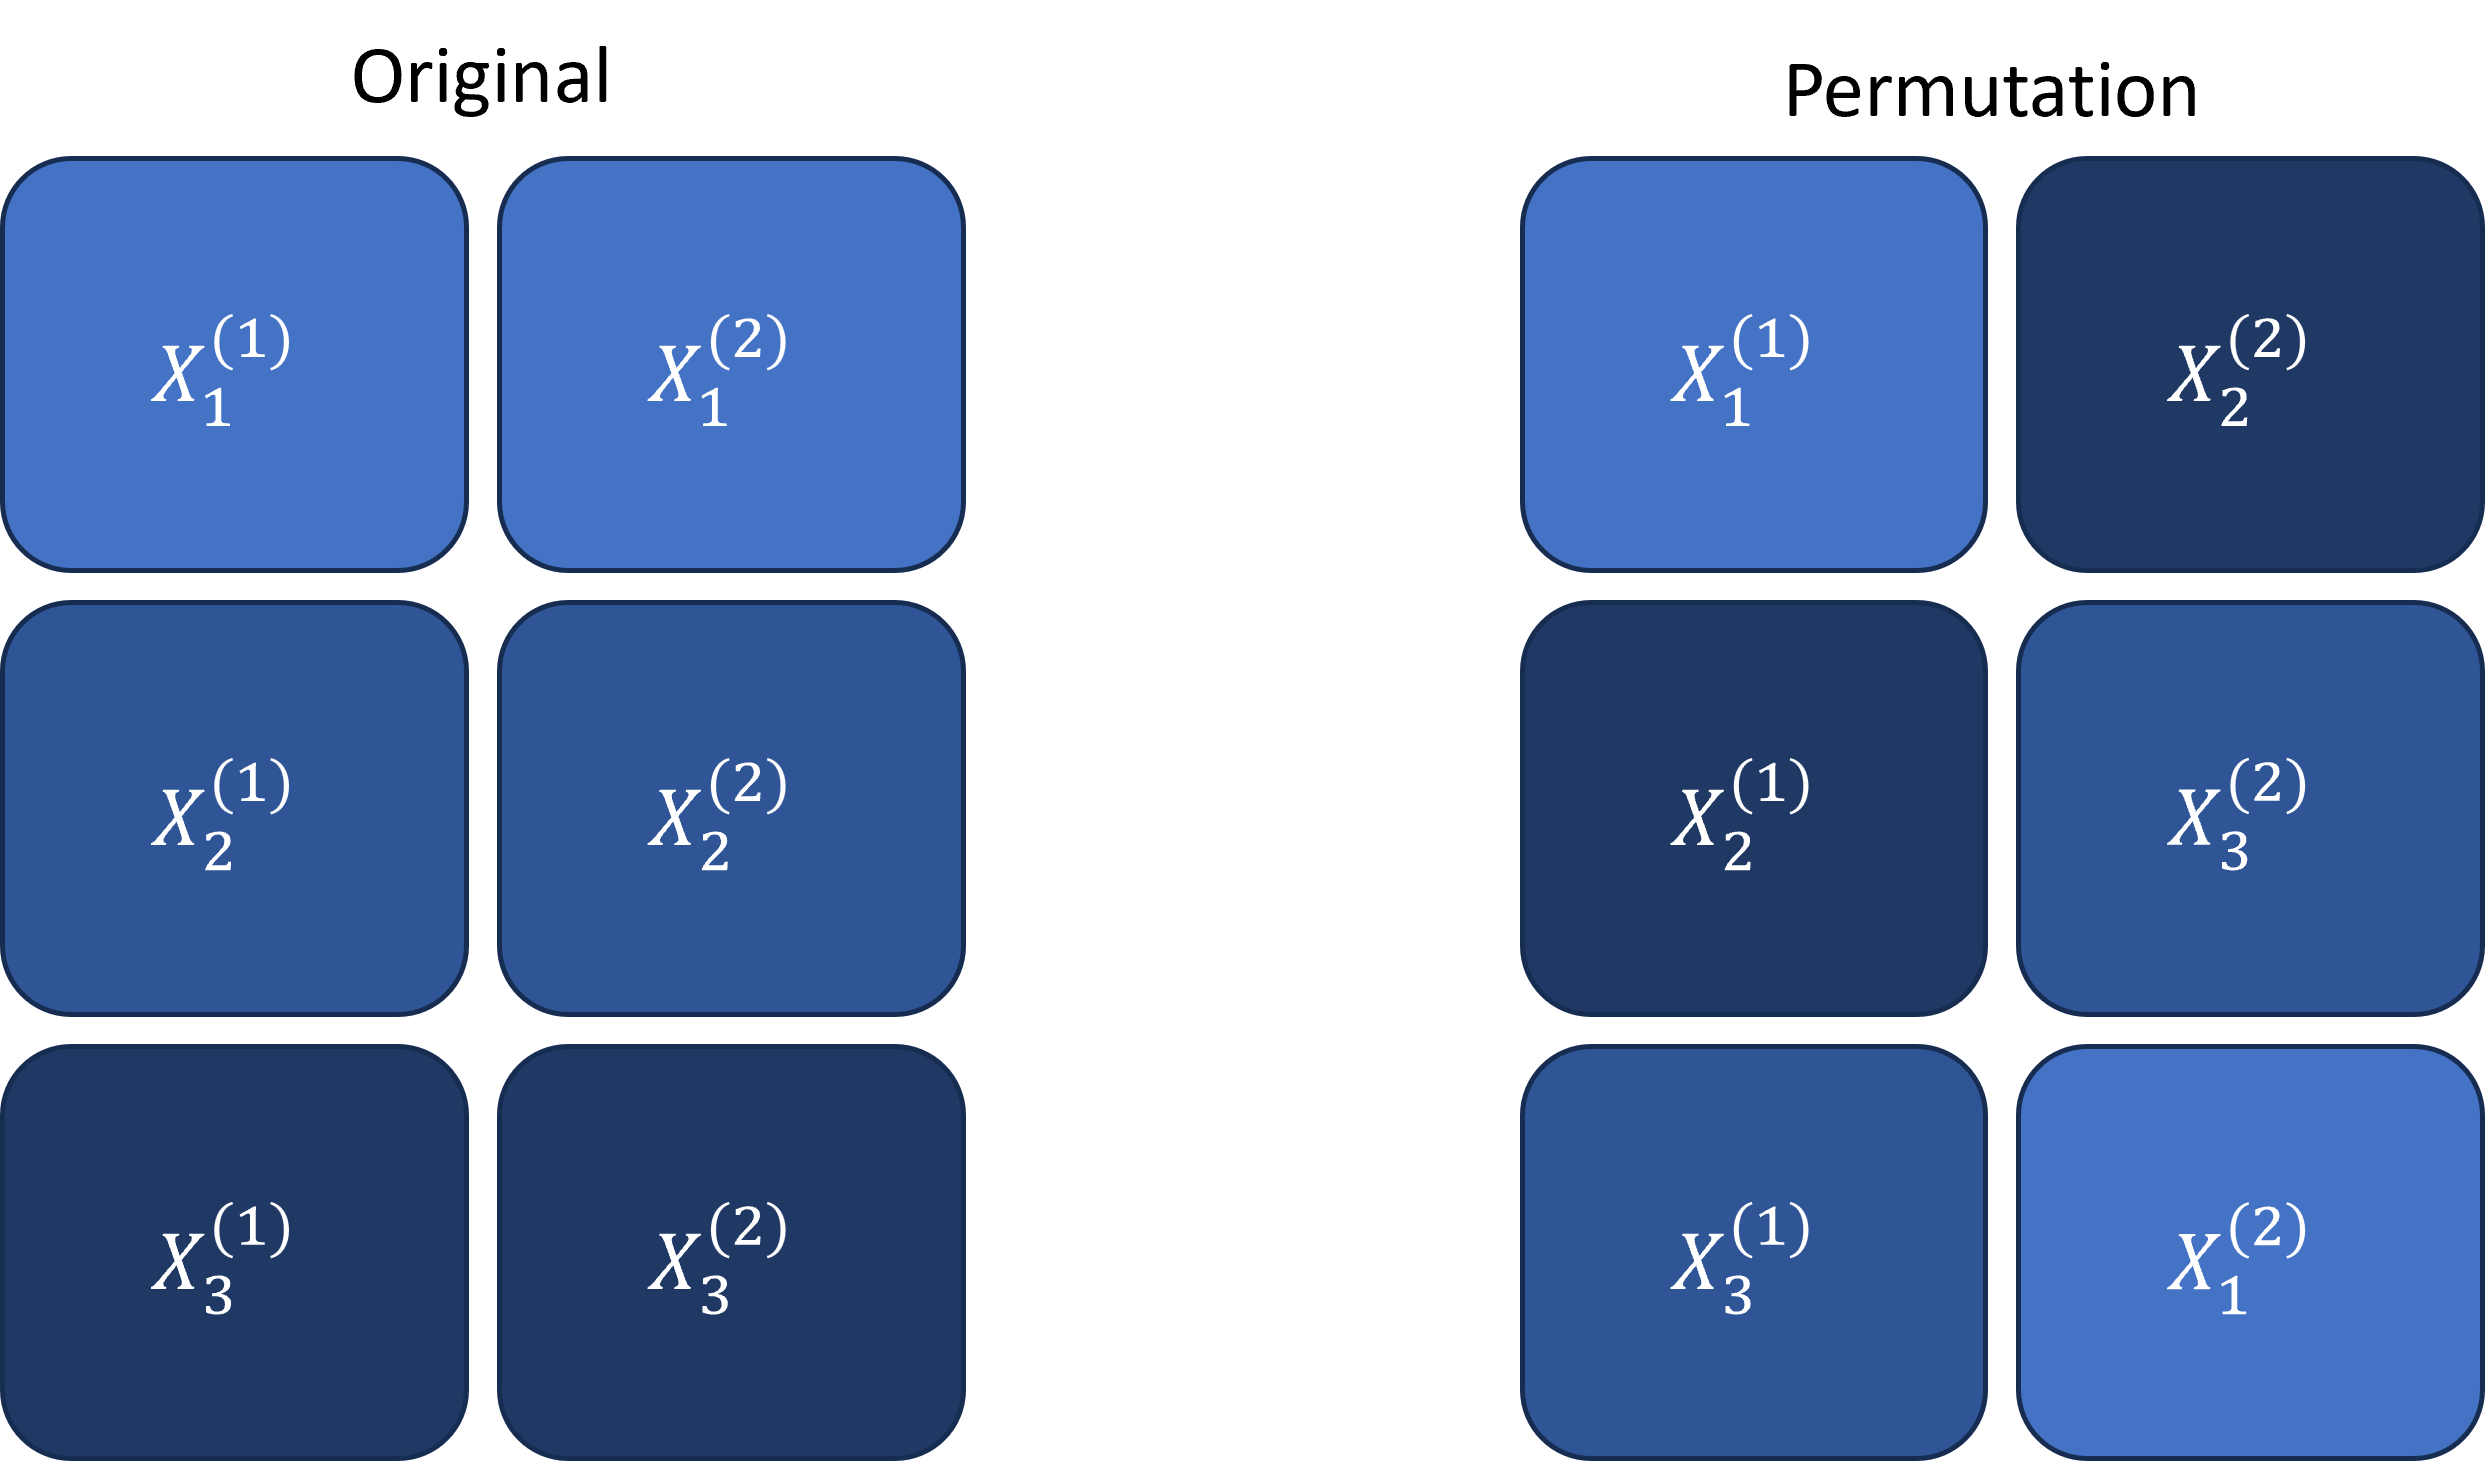
\includegraphics[width=0.8\textwidth]{figures/permutation_test.png}
    \caption{Schematic of the permutation testing procedure. The original data are randomly shuffled, and the model is retrained on the shuffled data. This process is repeated multiple times, and the model's performance on the original data is compared to the distribution of performances on the shuffled data.}
    \label{fig:statistical-inference}
\end{figure}

Permutation testing offers a robust way to evaluate the significance of the results obtained by multiview learning methods and, for a single component, is a relatively simple process \citep{winkler2020permutation}.
As illustrated in Figure~\ref{fig:statistical-inference}, the views are randomly and separately shuffled, and the model is then trained and tested on this permuted data.
This process is repeated multiple times, generating a distribution of performance metrics under the null hypothesis, where there is no relationship between the views.
The actual performance of the model on the unshuffled data is then compared to this distribution.
If the actual performance is significantly better than the permuted performance, it suggests that the model is capturing meaningful relationships in the data.

\subsubsection{Machine Learning}

\begin{figure}
    \centering
    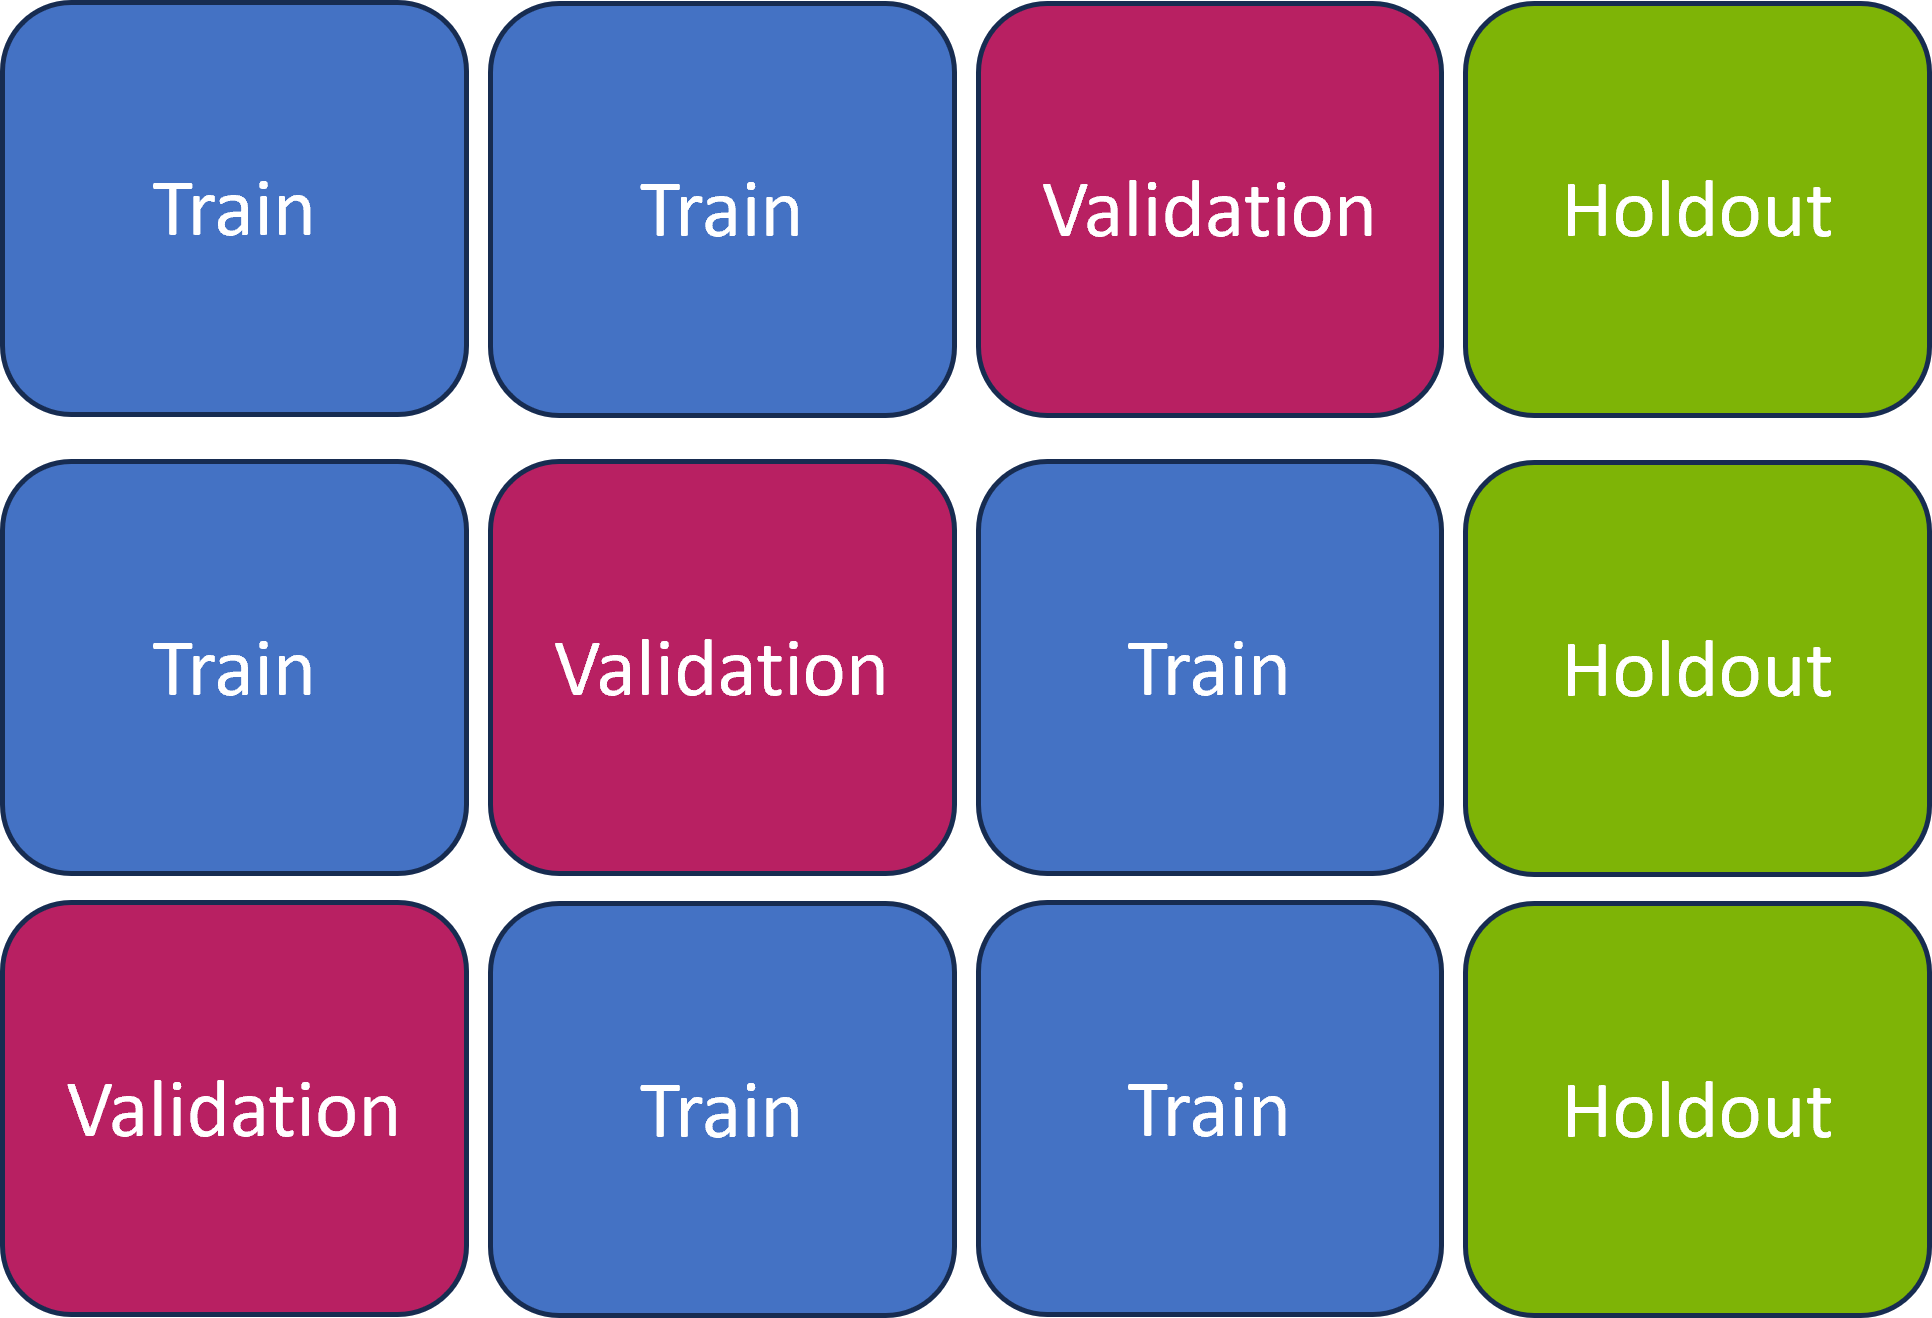
\includegraphics[width=0.8\textwidth]{figures/cross-validation.png}
    \caption{Schematic of the cross-validation procedure. The original data are partitioned into training and test sets. In cross-validation, the training set is further partitioned into training and validation sets. The model is trained on the training set and evaluated on the validation set for different parameter values. The parameter value with the best performance on the validation set is selected, and the model is retrained on the entire training set. The final model is evaluated on the single test or holdout set.}
    \label{fig:machine-learning}
\end{figure}

The machine learning approach to evaluating multiview learning methods is to use a holdout or test set to estimate the out-of-sample performance of the model.
Within the training set, where necessary, cross-validation is used to select the best model hyperparameters.
Cross-validation involves partitioning the training set into training and validation sets, training the model on the training set, and evaluating the model on the validation set.
When this is performed for multiple subsets of the training set, it is referred to as \(k\)-fold cross-validation as illustrated in figure \ref{fig:machine-learning}.
The model hyperparameters are then selected based on the performance across the validation sets.
The model is then retrained on the entire training set using the best hyperparameters, and evaluated on the test set.

In this thesis, we will use the machine learning approach throughout.
This is because in scaling up to large datasets, permutation testing becomes computationally intractable.
This is because permutation testing requires retraining the model multiple times on the permuted data.
This comes at the cost of only being able to evaluate models with a point estimate of performance, rather than a distribution.
In chapter \ref{ch:loadings}, we observe and argue that signals of interest have a large effect size, and therefore permutation testing is not necessary to evaluate the significance of the results.

\subsection{Components and Subspaces in CCA}

\subsubsection{Eigenvalue Problems in CCA}

While our focus so far has primarily been on the top-1 eigenvector-eigenvalue pair, it's important to note that the methodology also extends to the top-k subspace problem. This broader approach involves identifying the top-k eigenvectors and their corresponding eigenvalues.

\subsubsection{Addressing the Top-k Problem}

Transitioning from a focus on the top-1 component to exploring the top-k subspace introduces additional complexities. One common method to solve the top-k problem is to identify the top-1 component and then apply a deflation process to find subsequent orthogonal components.
Deflation involves removing the top-1 component from the data and then repeating the process to find the next top-1 component. This process is repeated until the desired number of components is found.
For instance, Hotelling's Deflation \citep{hotelling1933analysis} involves removing the top-1 component from the data, while Projection Deflation \citep{mackey2008deflation} involves projecting the data onto the orthogonal complement of the top-1 component.
Different deflation methods enforce different forms of orthogonality, which can impact the resulting components and their interpretation, particularly when the first component is not a true eigenvector.

\subsubsection{Non-Uniqueness of Components}

Furthermore, non-uniqueness is a significant challenge in representation learning, particularly when eigenvectors have repeated eigenvalues. Imagine a scenario where the top-1 eigenvalue is repeated \(k\) times. In this case, there are \(k\) possible eigenvectors that can be associated with the top-1 eigenvalue. While this is unlikely to occur in practice, the eigenvalues can in practice be very close to each other, leading to numerical instability and non-uniqueness in the components. Particularly true in cross-validation settings, this non-uniqueness can lead to instability in the components, complicating their interpretation and comparison.
For example, the top-1 component in one analysis might be the second component in another analysis, making it difficult to compare the results.

This non-uniqueness also has a grounding in the probabilistic perspectives on PCA and CCA (introduced in chapter \ref{ch:loadings}), where the latent variables are considered unique only up to a rotation.
This perspective further reinforces the subspace approach, emphasizing the identification of a subspace rather than specific directions within it.

\paragraph{Thesis Approach: Concentrating on the Top-1 Component}

In this thesis, we focus on the top-1 component in CCA to align with and facilitate comparison with typical componentwise studies in brain-behavior research.
This choice is driven by the complexity associated with the top-k problem and the variety of methods available to address it.
Under the assumption of a significant eigengap\footnote{An `eigengap' refers to the difference in magnitude between consecutive eigenvalues in an eigenvalue problem. A significant eigengap between the first and second eigenvalues suggests that the first eigenvalue (and its corresponding eigenvector) is distinctly more significant than the next, lending credence to its uniqueness and importance.}, the first component can be considered equivalent to the top-1 subspace.
This equivalence allows for a clear and interpretable analysis, making the top-1 subspace a straightforward and reliable choice for studying multivariate data.
It is important to note that while we focus on the top-1 component, the later sections of the thesis introduce a method for simultaneously solving the complete subspace, addressing broader subspace analyses.


\section{Multiview Learning in Neuroimaging}

Finally, we review important applications of multiview learning from the literature in neuroimaging, which will be our reference in chapters \ref{ch:als} and \ref{ch:loadings}.

\subsection{Multiview Data in Neuroscience and Genetics}

In neuroscience and genetics, two specific types of multiview studies are particularly relevant to this thesis: brain-behavior studies and imaging-genetics.
Both involve the integration of data from multiple sources, offering rich insights into complex phenomena.

Brain-behavior studies typically involve pairing neuroimaging data, such as that obtained from Structural MRI (sMRI) or Functional MRI (fMRI), with non-imaging data like responses from questionnaires, cognitive test results, and other behavioral assessments.
sMRI provides detailed anatomical brain images, essential for understanding brain structure and neurological disorders \citep{kanai2011structural}, while fMRI focuses on brain function by mapping activity during cognitive tasks \citep{miranda2021systematic}.
The integration of these imaging techniques with behavioral data offers a comprehensive view of how brain structures and functions correlate with behavioral and cognitive patterns \citep{rypma2001age,genon2022linking}.

Imaging-Genetics, another critical multiview approach, combines neuroimaging data with genetics and omics information \citep{le2008sparse}.
This interdisciplinary field seeks to understand the genetic influences on brain structure and function, thereby illuminating the genetic basis of neuropsychiatric disorders and cognitive traits \citep{bogdan2017imaging}.
Studies in this area can explore how specific genetic variations correlate with differences in brain morphology or activity patterns observed in neuroimaging \citep{liu2014review}.

Together, these multiview approaches are fundamental in advancing our understanding of the brain's structure, function, and its interactions with genetic and behavioral factors.
They represent key applications of SSL in neuroscience and genetics, providing comprehensive insights that underpin developments in these fields.

\subsection{Applications of Multiview Learning in Neuroimaging}

There have been a number of applications of \acrshort{cca} and related methods to multiview problems in neuroimaging.
Using resting state fMRI data, modes of correlation have been found that relate to differences in sex and age relating to drug and alcohol abuse, depression and self harm \citep{mihalik2019brain}.
A similar mode relating to `positive-negative' wellbeing has been found across studies \citep{smith2015positive} suggesting that mental wellbeing has a relationship (though not necessarily causally) with functional connectivity between networks in the brain.
Later in this dissertation we will replicate and build on the findings from this paper by using regularised and non-linear \acrshort{cca} methods.
Owing to the high dimensionality of neuroimaging data, regularisation has been a particular focus of multiview learning in neuroimaging. \citet{mihalik2022canonical} reviews the application of \acrshort{cca} to neuroimaging data and highlights the importance of regularisation in this context. \citet{bilenko2016pyrcca} 
CCA has also been used as a preprocessing step in order to identify groups of subjects in the latent variable space.

In particular, \acrshort{cca} and clustering have been used to identify depression using fMRI data \citep{dinga2019evaluating,drysdale2017resting}.
CCA has also been used in the manner we described to denoise two \gls{views} of a dataset such as separate measures of neuroimaging data \citep{zhuang2020technical} to remove artefacts.
Deep \acrshort{cca} has recently been used to extract features for the diagnosis of schizophrenia\citep{qi2016deep}.

%\section{Open challenges in Multiview Learning and CCA}
%
%This thesis has been motivated by a number of open challenges in multiview learning and canonical correlation analysis.
%Chapter \ref{ch:als} and \ref{ch:loadings} will address the first challenge, which is the regularisation of \acrshort{cca} in high dimensional settings and the interpretation of the resulting components.
%Chapters \ref{ch:gradient_descent}, \ref{ch:deep_learning}, and \ref{ch:software} will address the second challenge, the efficient application of \acrshort{cca} to big data.
%Finally \ref{ch:deep_learning} will also address the third challenge, extending \acrshort{cca} to Deep Self-Supervised Learning.
%
%\subsection{Interpretability and Regularization}
%
%\textcolor{red}{TODO: Add a paragraph on interpretability and regularization}
%
%\subsection{Efficient Algorithms for High-Dimensional Data}
%
%\textcolor{red}{TODO: Add a paragraph on efficient algorithms for high-dimensional data}
%
%\subsection{Non-linear \acrshort{cca} and Joint Embedding Self-Supervised Learning}
%
%\textcolor{red}{TODO: Add a paragraph on non-linear \acrshort{cca} and Joint Embedding Self-Supervised Learning}
%
%







\chapter{Gradient Descent Based Formulations of Generalized Eigenvalue Problems for Multiview Subspace Learning: A Novel and Efficient Approach to Multiview Dimensionality Reduction}
\label{gradient descent}

The content of this chapter is based on a preprint paper where I am first author. I have extensively rewritten here in order to focus on the stochastic solution of Generalized Eigenvalue Problems. I initiated the project based on heuristic arguments and contacted coauthors Ana Lawry Aguila (who provided and analysed the UK Biobank data) and Lennie Wells (who provided extensive mathematical proofs which are in the appenix of this PhD thesis for the interest of the reader). Both of my coauthors helped me to revise the manuscript.

\section{Introduction}

using standard full batch algorithms to solve GEPs becomes very expensive with large-scale data, both in terms of memory and compute. This limits their applicability to many interesting modern datasets.
Therefore, there has been great interest in approximating the solution to these problems in the stochastic or data-streaming setting \cite{arora2012stochastic}.

\section{Background and Related Work}

\textbf{Stochastic GEPs}
Several methods have been proposed for solving GEPs with SGD.
\cite{arora2017stochastic} developed a Matrix Stochastic Gradient (MSG) method for finding the top-k CCA subspace, however its tractability relies on using minibatches of size 1. \cite{chen2019constrained} proposed a subspace Generalized Hebbian Algorithm (SGHA) which requires Lagrange multipliers. \cite{xie2015scale} propose a similar class of algorithms, but which estimate directions sequentially rather than as a subspace; \cite{chapman2022generalized} show there are also pseudo-objective based methods corresponding to this class of algorithms. More recently, the EigenGame line of work \cite{gemp20,gemp2021} has reframed the top-k subspace problem as a competitive game between components and recently extended the work to GEPs \cite{gemp2022generalized}. To our knowledge these are the state-of-the-art. However, there has been extensive other work tackling the top-1 problem in the stochastic CCA as well as stochastic PCA and PLS \cite{arora2012stochastic,arora2016stochastic,arora2017stochastic}.

\section{Method}

In this section, we introduce a new class of algorithms based on matrix analysis results which allow us to efficiently solve a number of interesting problems including but not limited to CCA, PLS, DCCA, and SSL.

\subsection{GEP-EY: an unconstrained objective for GEPs}\label{sec:gep-ey-formulation}
%old: A formulation of GEP problems by Matrix Analysis

First, we present GEP-EY, a formulation of GEP problems by matrix analysis which permits efficient optimization by gradient descent. 
This is summarised by proposition \ref{prop:EY-charac}, a consequence of applying the Eckhart-Young-Minsky inequality \cite{stewart_matrix_1990} to the eigen-decomposition of $B^\mhalf A B^\mhalf$. Detailed statements and proofs can be found in supplement \ref{supp:proofs}.
%L: of applying EY to the GEP formulation

\begin{restatable}[Eckhart-Young inspired objective for GEPs]{proprep}{EYcharac}
\label{prop:EY-charac}
    % The top-$k$ subspace of a positive semi-definite GEP $(A,B)$ can be characterised by:
    % \begin{align}\label{eq:EY-charac}
    %     \max_{W \in \R^{d \times k}} \mathcal{U}^\text{GEP-EY}(W) \defeq \tr \left( 2\, W^T A W - \left(W^T B W\right) \left(W^T B W\right) \right).
    % \end{align}
    The top-$k$ subspace of the GEP $(A,B)$ can be characterised by maximising the following objective over $W \in \R^{d \times k}$:
    \begin{align}\label{eq:EY-charac}
        \mathcal{U}^\text{GEP-EY}(W) \defeq \tr \left( 2\, W^T A W - \left(W^T B W\right) \left(W^T B W\right) \right)
    \end{align}
    Moreover, the maximum value is precisely $\sum_{j=1}^k \lambda_j^2$, where $(\lambda_j)$ are the generalised eigenvalues.
\end{restatable}

\subsection{CCA-SVD: an unconstrained objective for CCA}\label{sec:gep-ey-formulation}
% A formulation of CCA by Matrix Analysis
Next, we introduce CCA-SVD; a closely-related result that optimizes the SVD formulation of CCA and results in slightly more compact objectives which are cheaper to evaluate. It is summarized by proposition \ref{prop:SVD-CCA-charac}.

\begin{restatable}[SVD inspired objective for CCA]{proprep}{SVDCCAcharac}
\label{prop:SVD-CCA-charac}
    % The top-$k$ subspace for the CCA problem defined by $(\Sigxx,\Sigyy,\Sigxy)$ can be characterised by:
    % \begin{align}\label{eq:EY-charac}
    %     \max_{U \in \R^{p \times k}, V \in \R^{q \times k}} \mathcal{U}^\text{SVD-CCA}(U,V) 
    %     \defeq 2 \tr\left(U^T \Sigxy V \right) - \tr\left( U^T \Sigxx U \: V^T \Sigyy V \right)
    % \end{align}
    The top-$k$ subspace for the CCA problem defined by $X,Y \in \R^p,\R^q$ can be characterized by maximizing the following objective over $U \in \R^{p \times k}, V \in \R^{q \times k}$:
    \begin{align}\label{eq:EY-charac}
        \mathcal{U}^\text{SVD-CCA}(U,V) 
        \defeq 2 \tr\left({U}^T \Cov(X,Y) {V} \right) - \tr\left(\, {U}^T \Var(X) {U} \:\, {V}^T \Var(Y) {V} \,\right)
    \end{align}
    Moreover, the maximum value is precisely $\sum_{j=1}^k \rho_j^2$, where $(\rho_j)$ are the canonical correlations.
\end{restatable}

In the following sections, we describe a number of algorithms for solving GEPs using proposition \ref{prop:EY-charac}.
These will be denoted with \textbf{EY}. For the case of CCA, each of these algorithms have analogous forms using proposition \ref{prop:SVD-CCA-charac}, which will be denoted with \textbf{SVD}. However, describing both versions would muddle the exposition, and the GEP formulation is more general. We leave more detailed descriptions of the SVD-based forms to supplement \ref{supp:algorithm-details}.

\subsection{Stochastic Optimization}

We next show how GEP-EY and CCA-SVD can be efficiently optimized using stochastic methods, which makes them suitable for large-scale and online settings.
Suppose we have an unbiased estimate $\hat{A}$ for $A$ and a pair of independent and unbiased estimates $(\hat{B},\hat{B}')$ of the matrix $B$ (for example obtained from a minibatch); then one can estimate the objective in proposition \ref{prop:constr-charac} by:
\begin{align}
    \hat{\mathcal{U}}^\text{GEP-EY}(W) \defeq \tr \left( 2\, W^T \hat{A} W - \left(W^T \hat{B} W\right) \left(W^T \hat{B}' W\right) \right)
\end{align}
which we can differentiate to give a gradient estimate:
\begin{align}\label{eq:GEP-EY-grad}
    \hat{\Delta}^{\text{GEP-EY}}(W)
    \defeq \nabla_W \hat{\mathcal{U}}^\text{GEP-EY}(W)
    % old = 4 \left\{ \hat{A} W - \hat{B} W \left(W^T \hat{B}' W \right) \right\}
    = 2 \left\{ 2 \hat{A} W - \hat{B} W \left(W^T \hat{B}' W \right) - \hat{B}' W \left(W^T \hat{B} W \right) \right\}
\end{align}

By the independence of $(\hat{B},\hat{B}')$ both of these estimates are unbiased.

The unbiased estimate immediately leads to Algorithm \ref{alg:Delta}.
The key advantage of this is that the computational complexity of the algorithm is only $\mathcal{O}(b d k)$; this is far less than the $\mathcal{O}(N d^2)$ complexity of any methods which evaluate the matrices $A,B$ on the full batch.

\textit{Why is the complexity so low?} Because $A,B$ are linear functions of covariance matrices, we can construct our unbiased estimates by plugging in sample covariances on a minibatch.
These estimates will then be low rank; indeed we can factorise these estimates in the form $\hat{M} \hat{M}^T$ where $\hat{M} \in \R^{d \times b}$. The dominant cost in evaluating $\mathcal{U}^\text{GEP-EY}$ is then just the matrix multiplications of the form $\hat{M}^T W$; see supplement \ref{supp:analyticsubspace} for full details.

\begin{algorithm}
   \caption{GEP-EY: A Stochastic Gradient Descent Algorithm for GEP subspace}
   \label{alg:Delta}
\begin{algorithmic}
   \STATE {\bfseries Input:} data stream $Z_t$ consisting of B samples from $z_n$. Learning rate $(\eta_t)_t$. Number of time steps $T$. Number of eigenvectors to compute $k$.
   \STATE {\bfseries Initialise:} $(\hat{\mathbf {W}})_{i=1}^K$ with random uniform entries
   \FOR{$t=1$ {\bfseries to} $T$}
       \STATE Construct an independent unbiased estimate of $\hat{A}$ and two independent unbiased estimates of $\hat{B}$ from $Z_t$
        \STATE $\hat{\mathbf {W}} \leftarrow \hat{\mathbf {W}}+\eta_{t} \hat{\Delta}^{\text{GEP-EY}}$ 
        \COMMENT{As defined in (\ref{eq:GEP-EY-grad})}
   \ENDFOR
\end{algorithmic}
\end{algorithm}

\section{Experiments and Results}

%%%%%%%%%%%%%%%%%%%%%%%%%%%%%%%%%%%%%%%%%%%%%%%%%%%%%%%%%%%%%%%%%%%%%%%%%%%%%%%%%%%%%%
%Stochastic CCA
%%%%%%%%%%%%%%%%%%%%%%%%%%%%%%%%%%%%%%%%%%%%%%%%%%%%%%%%%%%%%%%%%%%%%%%%%%%%%%%%%%%%%%
\subsection{Application of GEP-EY and CCA-SVD to stochastic CCA}

In this section, we compare GEP-GD and CCA-SVD to $\gamma$-EigenGame \cite{gemp2022generalized} and SGHA \cite{chen2019constrained} for approximating CCA in the stochastic setting. Replicating the experiment in \cite{meng2021online, gemp2022generalized}, we optimize for the top-4 CCA subspace for the MediaMill and Split CIFAR (left and right halves of CIFAR-10 images) datasets. We use a minibatch size 100 and train for one epoch across 5 random seeds (with 1 standard deviation error bars in the plots). We use the Scipy \cite{virtanen2020scipy} package to solve the full batch GEPs as a ground truth value and use the proportion of correlation captured (PCC) captured by the learnt subspace as compared to this ground truth (defined in supplement \ref{supp:experimental details}). Unlike \cite{gemp2022generalized}, we do not perform PCA on the data before applying the CCA methods but instead, for the MNIST data, we add gaussian noise to avoid zero variance subspaces in $X$ and $Y$. This makes our task more challenging, as performing PCA simplifies the problem by substituting $B$ for the identity matrix $I$. This explains the decrease in performance of $\gamma$-EigenGame as compared to their original work.

Figure \ref{fig:ccaiter} shows that both of our methods outperform SGHA and $\gamma$-EigenGame on both datasets in terms of speed of convergence and achieve near-optimal performance in terms of PCC after just one epoch. All of the algorithms share the same complexity per iteration so that these results are also representative in terms of runtime. This demonstrates the effectiveness and superiority of our method for solving CCA in the stochastic setting.

\begin{figure}%[H]
     \centering
     \begin{subfigure}[b]{0.49\textwidth}
         \centering
         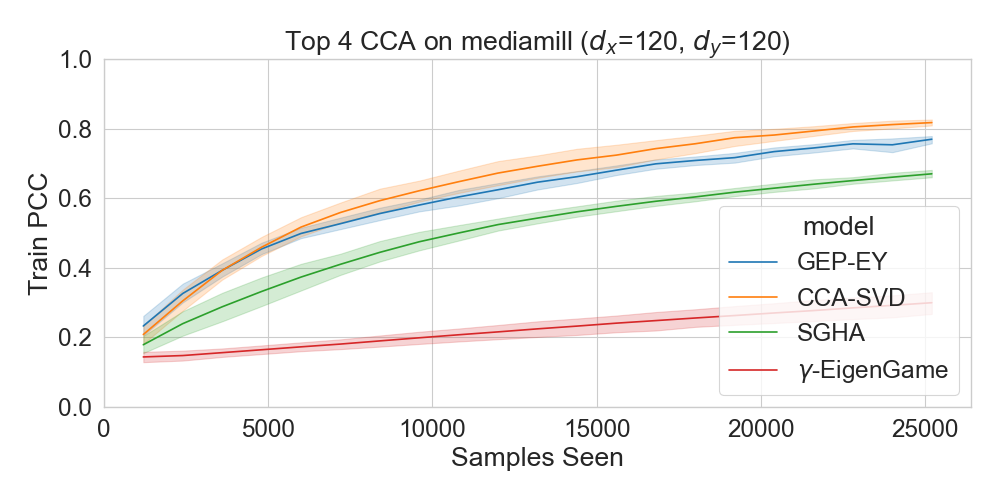
\includegraphics[width=\textwidth]{figures/CCA/mediamill_100_pcc_lr_tuned.png}
         \label{fig:ccamediamill}
     \end{subfigure}
     \hfill
     \begin{subfigure}[b]{0.49\textwidth}
         \centering
         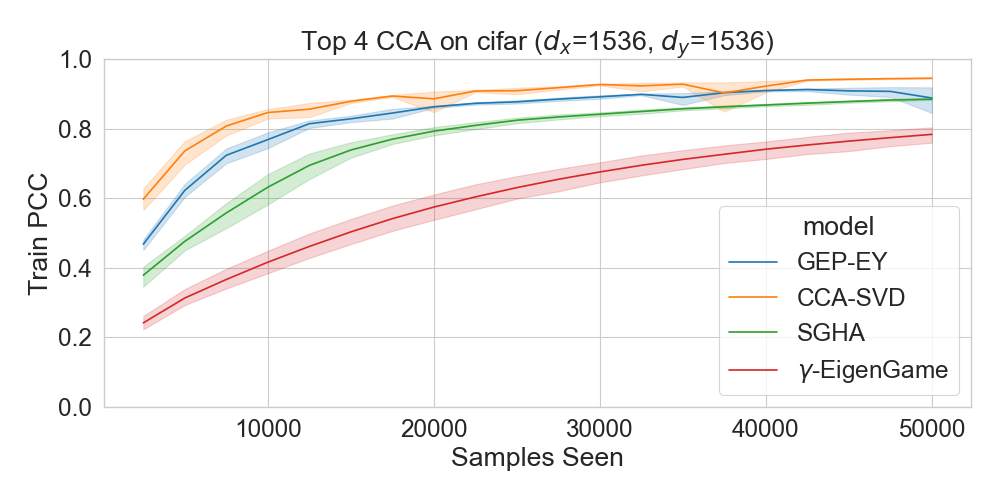
\includegraphics[width=\textwidth]{figures/CCA/cifar_100_pcc_lr_tuned.png}
         \label{fig:ccacifar}
     \end{subfigure}
        \caption{PCC with respect to Scipy ground truth by GEP-EY and CCA-SVD vs prior work for (a) MediaMill and (b) Split CIFAR data. The maximum value is 1.0 and shading represents $\pm$ 1 standard deviation.}
        \label{fig:ccaiter}
    \label{fig: stochasticcca}
\end{figure}

%Stochastic PLS UKBB
%%%%%%%%%%%%%%%%%%%%%%%%%%%%%%%%%%%%%%%%%%%%%%%%%%%%%%%%%%%%%%%%%%%%%%%%%%%%%%%%%%%%%%
\subsection{Application of GEP-EY to PLS on large scale biomedical data}

We demonstrate the power of GEP-EY for large-scale subspace learning by solving PLS on imaging genetics data from the UK Biobank \cite{sudlow2015uk}, a biomedical database. This can reveal novel phenotypes of interest and uncover genetic mechanisms of disease and brain morphometry. Previous imaging genetics analyses using PLS and CCA were limited to small-scale datasets \cite{Lorenzi2018,Taquet2021,Lefloch2012}, which are prone to overfitting and instability. Full batch approaches are infeasible for this data due to the high computational cost. The only other large-scale PLS analysis on the UK Biobank used a federated approach with local batch PLS-SVD \cite{lorenzi2016}, which approximates the global solution. We present the first stochastic PLS analysis on large-scale biomedical data.

We ran GEP-EY with minibatch size 500 on brain imaging (82 regional volumes) and genetics (582,565 variants) data for 33,333 subjects; a massive amount of data that challenges existing methods. See supplement (Section \ref{sec:ukbb_preprocessing}) for data pre-processing details. We see strong validation correlation between all 10 corresponding pairs of vectors in the PLS subspace and weak cross correlation, indicating that our model learnt a coherent and orthogonal subspace of covariation (Figure \ref{fig:UKBB_corr}), a remarkable feat for such high-dimensional data. We found that the PLS brain subspace was associated with genetic risk measures for several disorders (Figure \ref{fig:genetic_risk}), suggesting that the PLS subspace encodes relevant information for genetic disease risk, a significant finding for biomedical research.


\begin{figure}
\centering
     \begin{subfigure}[b]{0.27\textwidth}
         \centering
          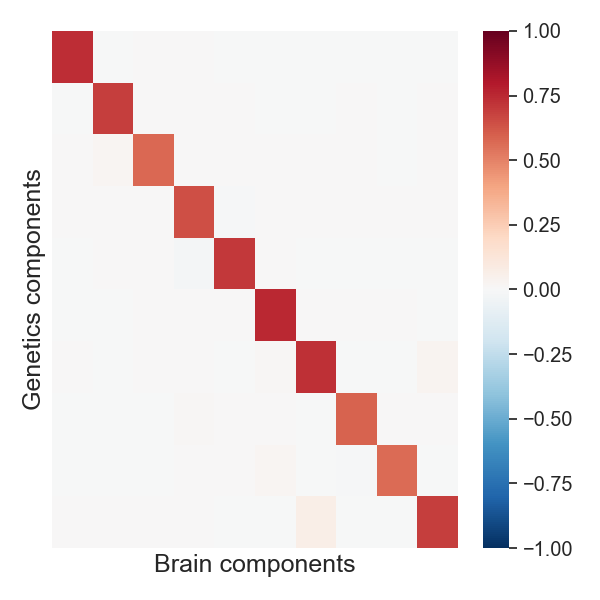
\includegraphics[width=\textwidth,trim={0.8cm 0cm 0.3cm 0cm}]{figures/UKBB/cross_corr.png}
          \caption{}
          \label{fig:UKBB_corr}
     \end{subfigure}
     \begin{subfigure}[b]{0.72\textwidth}
         \centering
          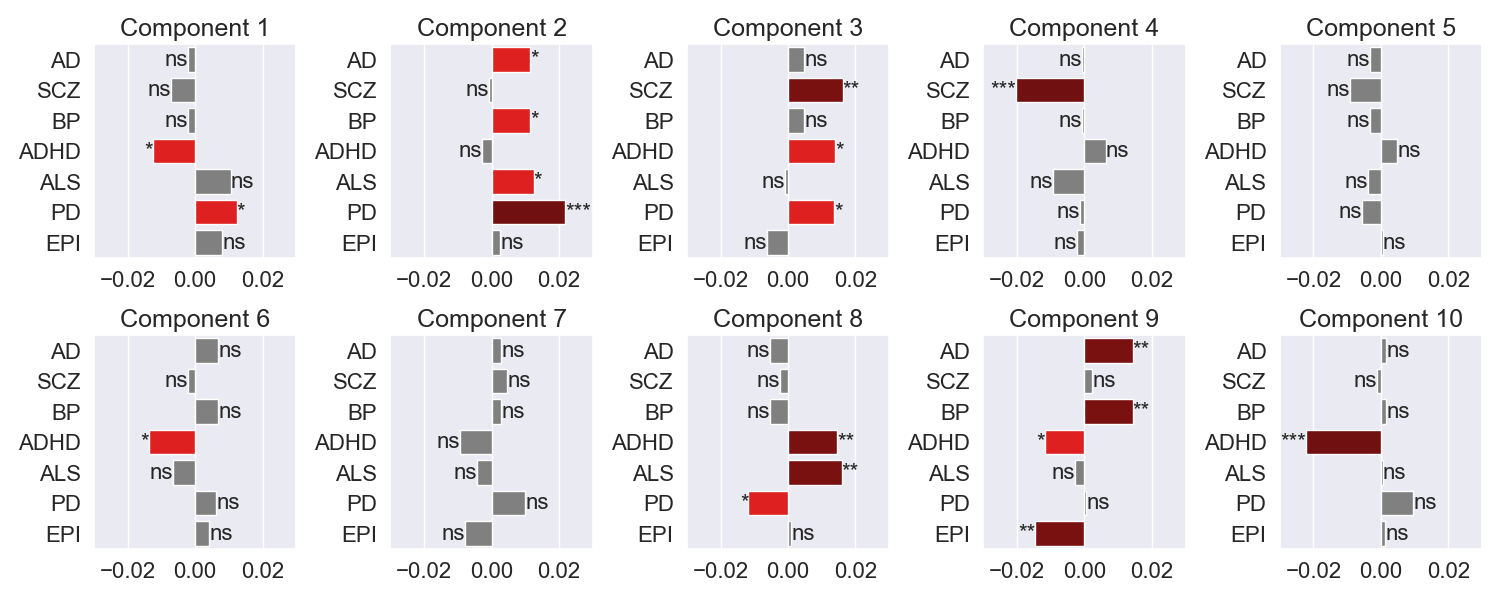
\includegraphics[width=\textwidth,trim={0.5cm 0cm 0.7cm 0cm}]{figures/UKBB/prs_correlations.png}
          \caption{}
          \label{fig:genetic_risk}
     \end{subfigure}
\caption{(a) Correlations between PLS components for UK Biobank. (b) Correlations between PLS brain components and genetic risk scores. AD=Alzheimer's disease, SCZ=Schizophrenia, BP=Bipolar, ADHD=Attention deficit hyperactivity disorder, ALS=Amyotrophic lateral sclerosis, PD=Parkinson's disease, EPI=Epilepsy. $\text{ns}: 0.05< p <= 1, \ast: 0.01< p <=0.05, \ast\ast: 0.001< p <= 0.01, \ast\ast\ast: 0.0001< p <= 0.001$.}
\end{figure}

\section{Discussion and Conclusion}

We presented a new unconstrained objective to characterise GEPs; this immediately gave efficient algorithms to solve many subspace learning methods in the stochastic setting with SGD.
Crucially, the gradient estimates are unbiased and cheap to compute. Moreover, the only hyperparameter is the choice of optimiser.

We will later show how this work can be adapted and applied to optmise regularised GEPs and in particular CCA.

\chapter{Flexible, Scalable Regularization for Generalized Eigenvalue Problems for Multiview Subspace Learning}
\label{Regularised}

The content relating to regularised alternating least squares as a method for optimizing regularised CCA is based on an abstract which I presented in poster form at OHBM. The work benefitted from extensive theoretical discussions with John Shawe-Taylor and Janaina Mourao-Miranda as well as Janaina and Rick Adams' help interpreting the results.

\section{Introduction}


\section{Background and Related Work}

\section{Related Work}

In this section we review some existing regularised CCA methods including some of the existing extensions to data with more than two views. Since almost all of the existing work considers sparsity inducing regularisation this is the main focus.

There have been many different proposals in the literature for finding sparse regularised solutions. In this section, we describe the penalized matrix decomposition method (arguably the most common in applied sparse CCA) as well as some of the methods based on least squares formulations. Like the unregularised CCA and PLS formulations, they can broadly be grouped into penalized SVD based methods and penalised iterative methods.

\subsection{Penalized Matrix Decomposition}\label{sec:witten}

Witten's "Penalized Matrix Decomposition" (PMD) \cite{witten2009penalized} approach substitutes the CCA constraints $\bold{w_i^{\top}X_i^{\top}X_iw_i}=1$ for the PLS constraints $\bold{w_i^{\top}w_i}=1$. This is equivalent to assuming that the variance-covariance matrix of $X$ is an identity matrix or in other words that the columns of the original data matrices are independent. This subtle change means that Witten's method introduced in this paper is only an approximation to a sparse CCA optimisation problem. It follows that this method will perform best (in terms of optimising the `true' CCA objective) when the identity covariance matrix assumption is strongest. In addition, much as with PLS, PMD is biased towards the largest principal components in the data and will select directions with high covariance even if they are not the maximally correlated directions.

Since the PLS constraint $\bold{w_1^{\top}w_1}=1$ is non-convex, Witten further relaxes this constraint to an inequality. The penalized matrix decomposition can then be expressed as the constrained optimization problem in \ref{eq:pmd}. 

\begin{align}
    \label{eq:pmd}
    & \bold{w_{opt}}=\underset{\bold{w}}{\mathrm{argmax}}\{ \bold{w_1^{\top}X_1^{\top}X_2w_2} \}\\
    & \text{subject to:} \notag\\
    & \bold{w_1^{\top}w_1}\leq1 \notag\\
    & \bold{w_2^{\top}w_2}\leq1 \notag\\
    & P(\bold{w_1})\leq c_1 \notag\\
    &P(\bold{w_2})\leq c_2 \notag
\end{align}

Where $P(\bold{w_1})=\|\bold{w_1}\|_1$ would form a constraint on the 1-norm but in principle the algorithm only requires that $P(\bold{w_1})$ is a one-homogenous function:

\begin{align}
    & \lambda P(\bold{w})=P(\lambda \bold{w})
\end{align}

In order to solve this optimisation, Witten proposed an algorithm based on a rank 1 singular value decomposition of a matrix $\bold{M}=\bold{X_1^{\top}X_2}$. Since soft-thresholding is equivalent to Lasso when $\bold{X_i^{\top}X_i}=\bold{I}$, the algorithm is simply the power method for singular value decomposition with soft-thresholding applied at each iteration such that $\|\bold{w_i}\| \leq c_i$. The soft-threshold function can be written as:

\begin{align}
    \label{eq:softthreshold}
    & S(x,\gamma) = \text{sign}(x)\text{max}(0,\|\bold{x}\|-\gamma)
\end{align}

Where $\gamma$ defines the threshold of the absolute value below which coefficients in $x$ are set to zero. We can then iteratively find the threshold $\gamma$ that fulfils the l1-norm condition using for example binary search:

\vspace{\baselineskip}
\begin{algorithm}[H]
\begin{algorithmic}
\STATE {Finds local optima for sparse left and right eigenvectors of the covariance matrix} $X_1^{\top}X_2$
\STATE $M_1=X_1^{\top}X_2$
\FOR {$k \gets 1$ \textbf{to} $K$}
    \STATE Initialize $|w^{(k)}_2|_2=1$
    \WHILE {Not converged}
        \STATE $w^{(k+1)}_1=M_kw^{(k)}_2$
        \STATE $w^{(k+1)}_1=S(w^{(k+1)}_1,\gamma)$
        \STATE $w^{(k+1)}_1=\frac{w^{(k+1)}_1}{\|w^{(k+1)}_1\|_2}$
        \STATE $w^{(k+1)}_2=M_k^{\top}w^{(k+1)}_1$
        \STATE $w^{(k+1)}_2=S(w^{(k+1)}_1,\gamma)$
        \STATE $w^{(k+1)}_2=\frac{w^{(k+1)}_2}{\|w^{(k+1)}_2\|_2}$
        \STATE $M_{k+1}=M_k-du_kv_k^{\top}$
    \ENDWHILE
\ENDFOR
\caption[Penalized Matrix Decomposition]{Penalized Matrix Decomposition for CCA}
\end{algorithmic}
\end{algorithm}
\vspace{\baselineskip}

Witten also showed that the lasso constraint could be replaced with a fused lasso constraint by replacing the soft-threshold with an appropriate update step.

\subsection{Penalized CCA}

Parkhomenko proposed a similar algorithm to penalized matrix decomposition, substituting the covariance matrix $\bold{X_1^{\top}X_2}$ for the correlation matrix $\bold{(X_1X_1^{\top})^{-\frac{1}{2}}X_1^{\top}X_2(X_2^{\top}X_2)^{-\frac{1}{2}}}$\cite{parkhomenko2009sparse}. However their soft-thresholding step uses the threshold as the hyper-parameter and therefore cannot be written as a constrained optimization problem. For this reason it is also difficult to select an appropriate range for the hyperparameters $\gamma_i$ as this is more dataset dependent:

\begin{align}
    \label{eq:parkho}
    & \bold{w_{opt}}=\underset{\bold{w}}{\mathrm{argmax}}\{ \bold{(X_1X_1^{\top})^{-\frac{1}{2}}X_1^{\top}X_2(X_2^{\top}X_2)^{-\frac{1}{2}}} \}
\end{align}

While this makes the optimisation more CCA-like than PLS-like, it requires us to calculate the inverses $\bold{(X_1X_1^{\top})^{-\frac{1}{2}}}$ and $\bold{(X_2^{\top}X_2)^{-\frac{1}{2}}}$. However in cases where the number of features $p$ is greater than the number of samples $n$, as is common in many applications of sparse modelling such as neuroimaging, these matrices cannot be inverted. 

For this reason, Parkhomenko recommended diagonalising the covariance matrices $\bold{X_i^{\top}X_i}$ or making them identity matrices. Witten's method can thus be seen as an extremely regularised version of Parkhomenko's. 

\subsubsection{Alternating Least Squares}\label{sec:ALS}

Since the scale invariance constraints in the CCA optimisation problem can also be represented by the unconstrained objective: 

\begin{align}
    & \bold{w_{opt}}=\underset{\bold{w}}{\mathrm{argmax}}\{\bold{\frac{\bold{w_1^{T}X_1^{T}X_2w_2}}{\|\bold{X_1w_1}\|_{2}\|\bold{X_2w_2}\|_{2}}}\}
\end{align}

And since by adding constants to the objective we can show that maximising the objective is equivalent to minimising the distance between the two normalized projections \cite{golub1995canonical}:

\begin{align}
    \left\|\bold{\frac{X_1 w_1}{\|X_1 w_1\|_{2}}-\frac{X_2 w_2}{\|X_2 w_2\|_{2}}}\right\|_{2}^{2}=2\left(1-\bold{\frac{w_2^{T} X_2^{T} X_1 w_1}{\|X_2 w_2\|_{2}\|X_1 w_1\|_{2}}}\right)
\end{align}

We can transform the problem of maximising correlation to one of minimising the distance between the normalized projections $\bold{X_1w_1}$ and $\bold{X_2w_2}$.

This optimisation problem is convex in one variable when the other variable is fixed. Problems of this kind are referred to as biconvex (in the two variable case) and multiconvex (where it is true for more than two variables). They are typically optimized by iterating between these two convex problems, successively fixing $\bold{w_1}$ and solving for $\bold{w_2}$ and vice versa. This is referred to in this case as the "alternating least squares" method \cite{lykou2010sparse}. 

It is known that the alternating least squares algorithm is slower to converge when the 1st and 2nd canonical correlations (singular values of the covariance matrix $\bold{X_1^{\top}X_2}$) are closer together \cite{venkatg}.

\subsection{Iterative Penalized Least Squares for Sparse CCA}

There have been some proposals for sparse CCA that relate to the alternating regression form of CCA. Wilms originally proposed "sparse alternating regressions" \cite{wilms2015sparse} which replace the least squares problems at each iteration with lasso penalized regressions and a normalization step as shown in equation \ref{eq:SAR}:

\begin{align}\label{eq:SAR}
    & \bold{\hat{w}^{(i+1)}_1}=\underset{\bold{w}}{\mathrm{argmin}}\{ \|\bold{Xw-y}\|^2_2 + \lambda\|\bold{w}\| \}\\
    & \bold{w^{(i+1)}_1}=\bold{\frac{\hat{w}^{(i+1)}_1}{\|\hat{w}^{(i+1)}_1\|}}
\end{align}

It is clear that when the regularisation parameters $\lambda$ are set to zero we recover the alternating least squares CCA formulation. 

Mai offered a proof that the sparse alternating regression normalization step gave a true global solution to a projection-length constrained lasso regression\cite{mai2019iterative}:

\begin{align}
    & \bold{w}=\underset{\bold{w}}{\mathrm{argmin}}\{ \|\bold{Xw-y}\|^2_2 + P(\bold{w}) \}\\
    & \text{subject to:} \notag\\
    & \bold{w^{\top}X^{\top}Xw}=1 \notag
\end{align}

Furthermore, Mai showed that in principle the lasso penalty could be replaced with any one homogenous regularisation functional. The proof is sketched out as below:

\begin{thm}

For one-homogenous function $P(x)$, if the solution $\bold{\hat{w}}$ satisfies the unconstrained problem:

\begin{align}
    & \bold{\hat{w}}=\underset{\bold{w}}{\mathrm{argmin}}\{ \|\bold{Xw-y}\|^2_2 + P(\bold{w}) \}
\end{align}

Then the solution $\bold{w}$ to the constrained problem: 

\begin{align}
    & \bold{w}=\underset{\bold{w}}{\mathrm{argmin}}\{ \|\bold{Xw-y}\|^2_2 + P(\bold{w}) \}\\
    & \text{subject to:} \notag\\
    & \bold{w^{\top}X^{\top}Xw}=1 \notag
\end{align}

is equal to $\bold{w}=\bold{\frac{\hat{w}}{\|X\hat{w}\|}}$ or $\bold{w}=\bold{(\hat{w}^{\top}X^{\top}X\hat{w})^{-\frac{1}{2}}\hat{w}}$

\end{thm}

\begin{proof}

We have $c^2=\bold{\hat{w}^{\top}X^{\top}X\hat{w}}$. By definition we must also have $1=(c^{-1}\bold{\hat{w}^{\top})X^{\top}X(c^{-1}\hat{w})}$. Mai notes that the solution $\bold{\hat{w}}$ must also satisfy a constrained optimisation problem:

\begin{align}
    & \bold{\hat{w}}= \underset{\bold{w}}{\mathrm{argmin}}\{ \|\bold{Xw-y}\|^2_2 + P(\bold{w}) \}\\
    & \text{subject to:} \notag\\
    & \bold{w^{\top}X^{\top}Xw}=c \notag
\end{align}

By substituting the constraints, Mai shows that this is the same as finding:

\begin{align}
    & \bold{\hat{w}}=\underset{\bold{w}}{\mathrm{argmin}}\{ -\bold{y^{\top}Xw} + P(\bold{w)} \}\\
    & \text{subject to:} \notag\\
    & \bold{w^{\top}X^{\top}Xw}=c \notag
\end{align}

Where $c=1$ for the unit length constrained problem. Mai then defines:

\begin{align}
    & J(\beta)=-\bold{y^{\top}Xw} + P(\bold{w})\\
\end{align}

and uses the chain of inequalities:

\begin{align}\label{eq:maiinequalitychain}
    & J(\bold{w}) \leq J(c^{-1}\bold{\hat{w}})=c^{-1}J(\bold{\hat{w}}) \leq c^{-1}J(c^{-1}\bold{w}) = J(\bold{w})
\end{align}

To show that $J(c^{-1}\hat{\beta})=J(\beta)$. 

\end{proof}

\subsection{Elastic Penalized CCA}

In neuroimaging applications, we typically encounter highly correlated variables in the raw data. Since the sparse methods discussed so far may only select one of a number of highly correlated variables, a well known property of the lasso penalty, we may lose out on parts of the interpretability of the model. Waiijenborg proposed the use of elastic net regularisation in order to ensure group-level sparsity using the updates \cite{waaijenborg2008quantifying}:

\begin{align}
    & \bold{\hat{w}^{(i+1)}_1}=\underset{\bold{w_1}}{\mathrm{argmin}}\{(1+\lambda^{(1)}_2)\|\bold{X_1w_1-X_2w^{(i)}_2}\|^2_2 + \lambda^{(1)}_2\|\bold{w_1}\|^2_2 + \lambda^{(1)}_1\|\bold{w_1}\|_1 \}\\
    & \bold{\hat{w}^{(i+1)}_2}=\underset{\bold{w_2}}{\mathrm{argmin}}\{(1+\lambda^{(2)}_2)\|\bold{X_1w_1^{(i)}-X_2w_2}\|^2_2 + \lambda^{(2)}_2\|\bold{w_2}\|^2_2 + \lambda^{(2)}_1\|\bold{w_2}\|_1 \}
\end{align}

Where $\bold{\hat{w}}$ denotes unnormalized weights which are normalized in the same way as \ref{eq:SAR}. While the algorithm produces good results in practice, it has no theoretical guarantee of convergence or optimality and cannot simply be written as an optimization problem. In particular, as we showed in the previous section, normalizing the solutions to the unconstrained update equations in order to fulfil the projection-length constraint does not guarantee that we find a global optimum for the constrained optimization. 


\section{Contributions}

\subsection{Simulated Data for Comparing Sparse CCA Models}

A necessary 

\subsection{Flexible Regularised ALS}

We can solve CCA by alternating minimisation over each view, based on the alternating least squares form. This form finds a variable $\bold{T}$ that is close to the latent variables $\bold{X}_i\bold{W}_i$, where $\bold{X}_i$, $\bold{W}_i$ are the matrix and weights for each view $i$. The closer $\bold{T}$ is to $\bold{X}_i\bold{W}_i$, the higher the correlation between them. The constraint  $\bold{T^{\top}T}=\bold{I}$ ensures that the latent space is orthogonal to find different effects.

\[ \underset{\bold{W},\bold{T}}{\mathrm{argmin}}\left\{\sum_i \|\bold{X}_i\bold{W}_i-\bold{T}\|_{F}^2 \right\} \]
  \[ \text{subject to: } \bold{T^{\top}T}=\bold{I} \]

To regularise the projection matrices, we add penalty terms to the objective function, such as $P(\bold{W}_i)=\lambda_i\|\bold{W}_i\|_F$ for ridge regression or $P(\bold{W}_i)=\lambda_i\|\bold{W}_i\|_1$ for lasso. This can help us avoid overfitting and improve the interpretability of the results. This means that \textbf{any regularised least squares solver} can be used to solve each subproblem, such as ridge regression, lasso, elastic net, etc. making our framework substantially more flexible than prior work.

\[ \underset{\bold{W},\bold{T}}{\mathrm{argmin}}\left\{\sum_i \|\bold{X}_i\bold{W}_i-\bold{T}\|_{F}^2 + \textcolor{red}{\lambda_i P(\bold{W}_i)}\}\right\} \]
  \[ \text{subject to: } \bold{T^{\top}T}=\bold{I} \]

A benefit of this approach is that neuroimaging practitioners may have existing code for implementing specific regularisation methods in a regression context which can be reused. Furthermore, they may have large dimensions both in features and increasingly in number of samples which benefit from using highly optimised software. 

\subsection{Flexible Regularised GEPs by Proximal Gradient Descent}

\section{Experiments: Flexible Regularised ALS for Brain-Behaviour Associations in the Human Connectome Project}

\subsection{Experiment Design}

Using FRALS, we solve a CCA problem using alternating elastic net regressions with tuned l1 and l2 regularization. We compare our proposed framework to prior work including ridge Regularised CCA (RCCA), Penalized Matrix Decomposition (PMD), commonly referred to in the literature as Sparse CCA but which strictly optimises covariance rather than correlation, and separate Principal Components Analysis (PCA) of the brain and behavioural data. We show that our method improves on RCCA by finding sparse solutions and improves on PMD by optimising a correlation rather than covariance based objective.

We used resting-state fMRI and non-imaging subject measures of 1003 healthy subjects from the 1200-subject data release of the Human Connectome Project (HCP). Following the main steps from \cite{smith2015positive}, we processed the rs-fMRI data into brain connectivity matrices. Like \cite{smith2015positive} we used 145 items of the non-imaging subject measures and removed the same confounding variables. We split the data into 80\% train and 20\% test and used cross-validation within the training data in order to tune hyperparameters.

\subsection{Results}

\subsubsection{Out of sample generalization}

\subsubsection{Model Similarities}

\subsubsection{Brain Loadings}

\subsubsection{Behaviour Loadings}

\section{Experiments: Total Variation Regularisation using Simulated Data}
\subsection{Experiment Design}
\subsection{Results}


\section{Experiments: Total Variation Regularisation of Brain-Behaviour Assocations in the ADNI Data}
\subsection{Experiment Design}
\subsection{Results}

\section{Comparison of Sparse CCA Methods in Simulated Data}
\subsection{Experiment Design}
\subsection{Results}


\section{Discussion and Conclusion}




\chapter{Extending our work to Deep CCA and Self-Supervised Learning: A Powerful Approach to Multiview Nonlinear Association Learning}
\label{Deep}

\section{Introduction}


\section{Background and Related Work}

\subsection{Deep Learning}

With large amounts of data and improvements in hardware in recent years, `Deep' neural networks have become the state of the art in many tasks and in particular in computer vision. In principle, an infinitely wide neural network could model any function to arbitrary accuracy - a property known as the universal approximation theorem - and this flexibility allows neural networks to model complex relationships. 

In practice, rather than infinitely wide networks, `Deep' Neural Networks combine layers of linear weights with non-linear activation functions. Each layer can generally be written as a function of the outputs of the previous layer (or the raw input for the first layer):

$$
\bold{h_i}=s_i(\bold{W_ih_{i-1}}+\bold{b_i})
$$

Where we use the letter $h$ to denote a `hidden' layer or a representation between the input and output, $W$ to represent a matrix of weights, $b_i$ to represent a vector of bias terms and $s$, critically, to represent a non-linear activation function. One example of a non-linear activation function is the sigmoid function which maps linear outputs to a value between 0 and 1. Neural networks are often designed to have bottlenecks with fewer features in each subsequent hidden layer. This means that the outputs of each layer produce a hierarchy of features and it is often hypothesized that their generalisation ability is built upon producing these layers of abstraction\cite{li2018survey}. In general we will refer to the complete set of parameters (and architectural choices such as the number of layers) in a neural network with $\theta$. We therefore write a neural network function as $F(\bold{X};\theta_F)$.

The most common way to optimize neural networks is to use gradient descent (GD) in which we calculate the gradient of the network parameters with respect to some objective. When using the whole dataset to calculate the gradient we typically refer to `batch' gradient descent. However, when using non-linear functions, the objective is typically non-convex meaning GD is prone to finding local minima (regions in the parameter space where the gradient of the objective is zero) rather than global minima (local minima where the value of the objective is optimal). Perhaps for this reason, it is more effective to use Stochastic Gradient Descent (SGD), in which we estimate the gradient by using a single sample or a small set of samples referred to as a `minibatch'. This noisy estimate is less likely to get `stuck' in suboptimal solutions. Stochastic gradient descent mathematically relies on the stochastic estimate of the gradient being an unbiased estimate of the true gradient.

\subsection{Deep CCA}

Deep Canonical Correlation Analysis provides an alternative method to kernel CCA for finding complex non-linear structure in multiview data \cite{andrew2013deep}. In Deep CCA we look to use functions parameterized by neural networks $F(\bold{X};\theta_F)$ and $G(\bold{Y};\theta_G)$ to map the original data into a space in which the two views are maximally correlated. The problem we would like to solve is therefore:

\begin{align}
    & \theta_{F_{opt}},\theta_{G_{opt}}=\mathrm{argmax}\{\text{trace}( F(\bold{X};\theta_F)^{\top}G(\bold{Y};\theta_G))  \}\\
    & \text{subject to:} \notag\\
    & F(\bold{X};\theta_F)^{\top}F(\bold{X};\theta_F)=1 \notag\\
    & G(\bold{Y};\theta_G)^{\top}G(\bold{Y};\theta_G)=1 \notag
\end{align}

As we showed earlier in section \ref{sec:cca}, sum of the top $k$ canonical correlations of two views of a dataset can be shown to be the sum of the top $k$ singular values of the matrix $\bold{T}=\bold{\Sigma_{11}^{-\frac{1}{2}}\Sigma_{12}\Sigma_{22}^{-\frac{1}{2}}}$ where $\Sigma_{11}=F(\bold{X};\theta_F)^{\top}F(\bold{X};\theta_F)$. Now consider the identity $\|\bold{T}\|_*=\text{tr}(\sqrt{\bold{T^{\top}T}})$ known as the tracenorm of $\bold{T}$. This is symmetric and therefore can be diagonalised. Then since $T=\bold{U\Sigma V^{\top}}$:

\begin{align}
    & \|\bold{T}\|_*=tr(\sqrt{\bold{V\Sigma U^{\top}U\Sigma V^{\top}}})=tr(\sqrt{\bold{\Sigma^2 VV^{\top}}})=tr(\bold{\Sigma})
\end{align}

Therefore maximising the tracenorm maximises the total correlation between the representations.

\begin{figure}[H] %[H] "corresponds to start the figure Here"
    \centering %alignment can be flushleft, centering or flushright
    %includegraphics is the command to include graphics or pictures, [Width should be defined with respect to textwidth]{The path/ location of the image in the specified folder}, the image should be either in .png, .jpg, .pdf formats faster processing
    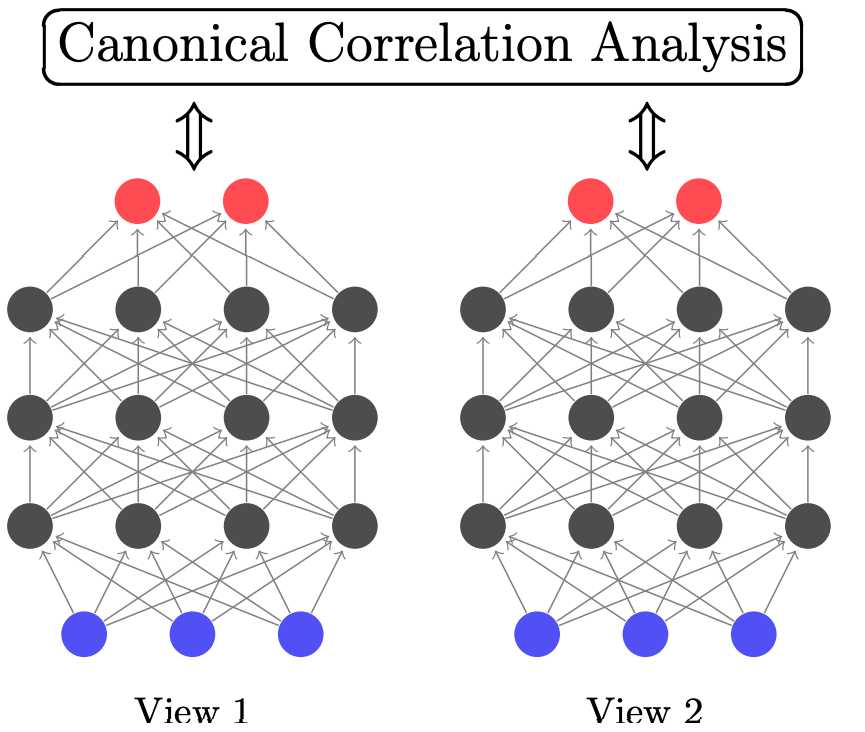
\includegraphics[width=0.5\textwidth]{chapters/litreview/DCCA.png} 
    \caption[Deep CCA Representation]{\textit{\textbf{Deep CCA with two correlated dimensions:}} A separate neural network is learnt for each view and a linear CCA is applied on top \cite{andrew2013deep}}
    \label{img:DCCA}
\end{figure}

A major problem with this DCCA formulation is that it relies on full-batch optimisation (optimized in the original paper by using the L-BFGS optimization algorithm). When gradients are calculated using smaller minibatches, the performance degrades drastically  because the estimation of the gradient is biased. In particular, mathematically the terms in $\Sigma_{ii}^{-\frac{1}{2}}$ are overestimated due to Jensen's inequality $E[\frac{1}{X}]>\frac{1}{E[X]}$. More intuitively, these matrices may be near singular for small samples causing stochastic gradients to blow up.

\subsection{Self-Supervised Learning}
\subsubsection{Barlow Twins}
%Relationship to CCA

\subsubsection{VICReg}
%Likewise


It is well known that VICReg and Barlow twins are closely related to CCA \cite{balestriero2022contrastive}. Similarly, \cite{kiani2022joint} showed how the SSL losses like VICReg could be adapted and implemented in closed form using the kernel method. Our work approaches the problem from the opposite angle, demonstrating how these classical problems can be extended to deep learning and solved with SGD without introducing bias.

\section{Methods}

\subsection{DCCA-EY and DCCA-SVD: Extension to Deep CCA}\label{sec:deep-cca}
The GEP-EY and CCA-SVD formulations also lead naturally to new formulations of Deep CCA which solve a more flexible CCA problem but unlike prior work can be optimized efficiently in the stochastic setting. We will refer to these as DCCA-EY and DCCA-SVD.

%L; just moved this up
We derive the DCCA-EY formulation by applying the GEP formulation of CCA (\ref{eq:cca-GEV}) to our DCCA definition. The analogous derivation for DCCA-SVD is left to supplement \ref{supp:algorithm-details}. 

Population DCCA \cite{andrew2013deep} can be defined analogously to population CCA (see section \ref{sec:CCA Definition}):
% Following the definition of CCA in section \ref{sec:CCA Definition}, the population formulation of DCCA \cite{andrew2013deep}, can be defined as follows: 
given input random vectors $X \in \R^{D_x}, Y \in \R^{D_y}$, find neural networks $f,g$ maximising:
\begin{align}\label{eq:DCCA-Andrew}
    \max_{f,g}  \norm{\CCA_K\left(f(X),g(Y)\right)}_2
\end{align}
% \in \mathcal{F}, g \in \mathcal{G}
% First we need to define the relevant matrices for our GEP. Consider $f,g$ as fixed for now, and define the (population) covariance matrices $\Sigma_{ff} = \operatorname{Var}(f(X)),\Sigma_{f,g} = \operatorname{Cov}(f(X),g(Y)),\Sigma_{gg}=\operatorname{Var}(g(Y))$. Then take
% \begin{equation*}
%     A_{fg} = \begin{pmatrix} 0 &\Sigma_{fg} \\ \Sigma_{gf} & 0 \end{pmatrix}, \qquad
% 	B_{fg} = \begin{pmatrix}\Sigma_{ff} & 0 \\ 0 & \Sigma_{gg}\end{pmatrix}
% \end{equation*}

The GEP formulation becomes:
\begin{equation*}
    A_{fg} = \begin{pmatrix} 0 &\Cov(f(X),g(Y)) \\ \Cov(g(Y),f(X)) & 0 \end{pmatrix}, \qquad
	B_{fg} = \begin{pmatrix}\Var(f(X)) & 0 \\ 0 & \Var(g(Y)) \end{pmatrix}.
\end{equation*}

Proposition \ref{prop:EY-charac} then allows us to rewrite our objective (\ref{eq:DCCA-Andrew}) as:
\begin{align*}
    % not quite equivalent to Andrew version without 1 extra small result
    %\max_{f \in \mathcal{F}, g \in \mathcal{G}}  \norm{\CCA_K\left(f(X),g(Y)\right)}_2
    %\max_{f,g,W} 
    \norm{\CCA_k\left(f(X),g(Y)\right)}^2 
    = \sum_{j=1}^k \rho_j^2 
    = \max_{W \in \R^{d \times k}} \tr \left( 2\, W^T A_{fg} W - \left(W^T B_{fg} W\right) \left(W^T B_{fg} W\right) \right).
\end{align*}
Therefore DCCA is equivalent to maximising the right hand side with respect to $f,g$ and $W$. To simplify the objective we follow \cite{wang2015stochastic} and reparametrize to consider the `augmented' neural networks $\bar{f} = U^{\top} f, \bar{g} = V^{\top} g$, where $U\in \R^{d_x \times k}, V\in \R^{d_y \times k}$ are such that $W^{\top} = (U^{\top}, V^{\top})$. This gives our final DCCA objective:

\begin{align}\label{eq:DCCA-EY}
    \mathcal{U}^\text{DCCA-EY}(\bar{f},\bar{g}) = \tr(2 \, A_{\bar{f}\bar{g}} - B_{\bar{f}\bar{g}} B_{\bar{f}\bar{g}})
\end{align}

where we need to define:
\begin{align*}
    A_{\bar{f}\bar{g}}
    &= W^T A_{fg} W 
    = \Cov(\bar{f}(X),\bar{g}(Y)) + \Cov(\bar{g}(Y),\bar{f}(X)) \\
    B_{\bar{f}\bar{g}} 
    &= W^T B_{fg} W 
    = \Cov(\bar{f}(X)) + \Cov(\bar{g}(Y))
\end{align*}

%L: there is a key difference in focus here - no longer have that the gradients are super cheap to compute in terms of the matrix dimensions, the dominant cost is going to be backprop through potentially fat $f,g$ rather than the final layer of $W$.
By plugging in sample covariances on a minibatch, we can obtain unbiased estimates of $\mathcal{U}^\text{DCCA-EY}(\bar{f},\bar{g})$.
% L: this is nit-picking and maybe obvious, but I missed it first time.
Therefore, we can apply some variant of SGD to optimize equation \ref{eq:DCCA-EY}.

Note that, as in the earlier DCCA work, though we derived the algorithm by considering $f,g$ with output dimensions $d_x,d_y$, we ultimately end up with networks $\bar{f},\bar{g}$ with the same output dimension $k$; we can view these as giving highly correlated $k$-dimensional embeddings of our data.
% Old: Note that, as in the earlier DCCA work, we ultimately end up with networks $\bar{f},\bar{g}$ which give us $k$ dimensional `latent' representations of our data. 
% L: I wrote this before but am no longer sure what it is doing here. There's something subtle about starting with $d_x$ NN outputs and only keeping $k$ directions...but it's what was done before

%maybe need extra stress on the interchange of expectation and differentiation / why it works, but maybe that's fine

%%% Unused ackground copied and pasted from Generalized Eigengame paper
%%% potentially will want to add in: 

% %augmented objective classes
% \begin{equation*}
%     \tilde{\mathcal{F}} = \{\bar{f} = U^{\top} f : f \in \mathcal{F}, U\in \R^{d_x \times k}\}, \quad
%     \tilde{\mathcal{G}} = \{\bar{g} = V^{\top} g : g \in \mathcal{G}, V\in \R^{d_y \times k}\}
% \end{equation*}

% % why putting tilde's on the Sigma's makes sense
% \begin{equation*}
%     U^{\top} \Sigma_{ff} U = \Sigma_{\bar{f}\bar{f}}, \quad
%     U^{\top} \Sigma_{fg} U = \Sigma_{\bar{f}\bar{g}}, \quad
%     V^{\top} \Sigma_{gg} V = \Sigma_{\bar{g}\bar{g}}
% \end{equation*}

\subsection{SSL-EY and SSL-SVD: Application to Self-Supervised Learning}

Finding highly correlated embeddings is a natural objective for SSL.
To apply the previous ideas to joint embedding methods, we simply apply (\ref{eq:DCCA-EY}) in the Siamese pair setting where $\bar{f}=\bar{g}$ are the same map from input data to embeddings (composition of encoder and projector).

% To apply these ideas to SSL, we suppose that our latent representations are learnt by 
% Finally, we introduce SSL-EY and SSL-SVD which adapt DCCA to the SSL setting in a principled way which permits greater understanding and, as we shall see, informs architecture choice.

% Following the 

% \begin{align*}
%     \tr 2 \left( \Cov(Z,Z') + \Cov(Z',Z) \right) - ...
% \end{align*}
% Consider the $f = h \circ g$ the encoder-expander composition.
% We will then apply (\ref{eq:DCCA-EY}) in the Siamese pair setting standard in SSL to enforce our embeddings to be highly correlated.

%Previously $X,Y$ were fundamentally different objects and we wanted to learn their relationship. In the SSL setting, we have $X, X'$ which are augmentations of the same object and we want to learn an embedding that is invariant to our data augmentations. For this reason, as is standard in SSL for computer vision, both views $X,X'$ share a neural network $f$.

We therefore obtain the objective:
\begin{align}\label{eq:SSL-EY}
    \mathcal{U}^\text{SSL-EY}(\bar{f}) =\tr( 2 \, A_{\bar{f}} - B_{\bar{f}} B_{\bar{f}})
\end{align}
where:
\begin{align*}
    A_{\bar{f}}
    &= \Cov(\bar{f}(X),\bar{f}(X')) + \Cov(\bar{f}(X'),\bar{f}(X)) \\
    B_{\bar{f}} 
    &= \Var(\bar{f}(X)) + \Var(\bar{f}(X')).
\end{align*}

Once again, we define SSL-SVD by analogy in supplement \ref{supp:algorithm-details}. We will see in section \ref{Experiments} that SSL-SVD and SSL-EY perform similarly in experiments but we show in supplement \ref{supp:previous work} that the SSL-SVD formulation looks closer to existing SSL methods.

\textbf{Implementation Details:} Typical architectures for the encoder and the projector vary depending on the domain and the dataset \cite{balestriero2023cookbook}. For example, for image classification tasks on CIFAR-10 or ImageNet, a common choice for the encoder is a ResNet, while for the projector a linear layer or a two-layer MLP is often used. Common augmentations for images are cropping, flipping, rotating, color jittering, etc. In this work, we adopt standard architectures and augmentations from the literature.


\section{Experiments and Results}

%%%%%%%%%%%%%%%%%%%%%%%%%%%%%%%%%%%%%%%%%%%%%%%%%%%%%%%%%%%%%%%%%%%%%%%%%%%%%%%%%%%%%%
%DCCA Benchmarking
%%%%%%%%%%%%%%%%%%%%%%%%%%%%%%%%%%%%%%%%%%%%%%%%%%%%%%%%%%%%%%%%%%%%%%%%%%%%%%%%%%%%%%
\subsection{Application of DCCA-EY and DCCA-SVD to to Deep multiview learning on toy data}

We now turn to compare our proposed DCCA-EY and DCCA-SVD methods with existing methods for deep canonical correlation analysis (DCCA). We replicate an experiment from \cite{wang2015stochastic} using the left and right halves of MNIST \cite{lecun1998gradient} digits ($n$=60,000) and X-Ray Microbeam (XRMB, $n$=1,429,236) data \cite{westbury1994x}. XRMB is a multimodal dataset of speech recordings from 139 speakers with acoustic and articulatory features. We use minibatch sizes of 100 for 20 epochs, the architectures described in \cite{wang2015stochastic}, and an output dimensionality of 50.  We use the total correlation captured (TCC) of the learnt subspace on the validation set as a metric (defined in supplement \ref{supp:experimental details}).

\begin{figure}
     \centering
     \begin{subfigure}[b]{0.49\textwidth}
         \centering
         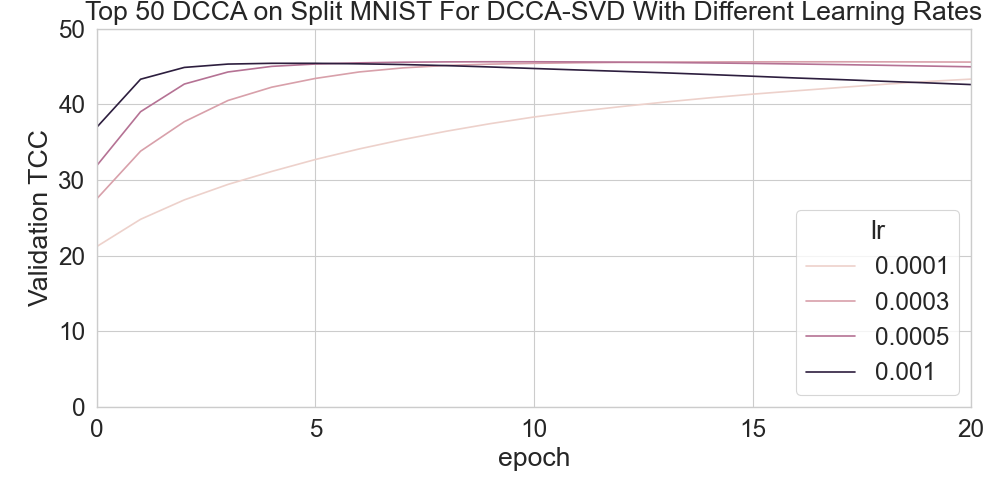
\includegraphics[width=\textwidth]{figures/DCCA/dcca_lr_experiment.png}
         \caption{}
         \label{fig:lrexp}
     \end{subfigure}
     \hfill
     \begin{subfigure}[b]{0.49\textwidth}
         \centering
         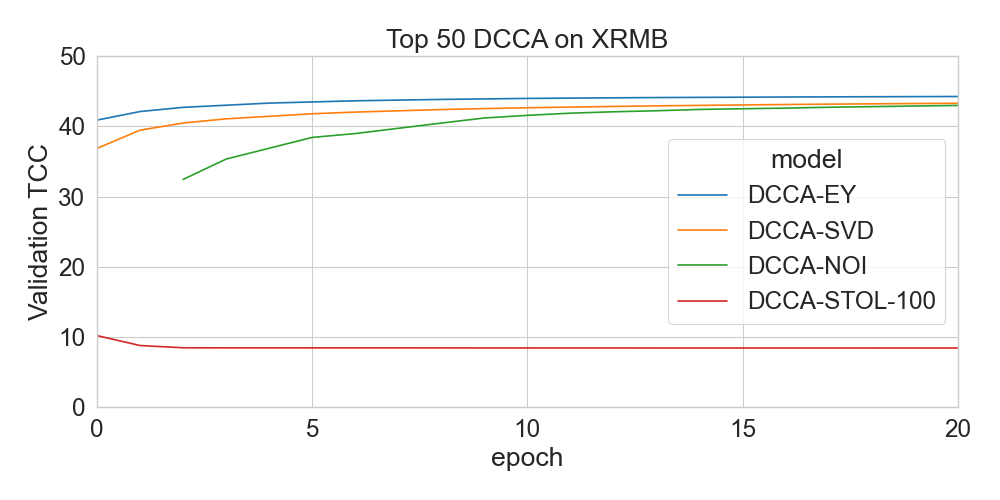
\includegraphics[width=\textwidth]{figures/DCCA/dcca_XRMB.png}
         \caption{}
                 \label{fig:xrmb}
     \end{subfigure}
        \caption{ (a) Validation TCC for different learning rates on Split MNIST data (b) Validation TCC for different methods on XRMB data}

\end{figure}

On the split MNIST data, we show in figure \ref{fig:lrexp} the substantial effect of changing the learning rate on the convergence of the TCC objective. This demonstrates the important of spending computational resource on optimizing the learning rate. An important benefit of our approach is that because the only hyperparameter is learning rate, we can spend all of our computational budget on this critical area. In figure \ref{fig:xrmb}, we show that our proposed methods exhibit extremely fast convergence compared to prior work. Furthermore, both proposed methods find higher validation correlations than DCCA-STOL, showing that they are much more effective ways of estimating the full batch DCCA objective. Note that, the decrease in validation correlation in later epochs is due to overfitting which should be addressed in practical settings by using early stopping as is standard in deep learning.

%%%%%%%%%%%%%%%%%%%%%%%%%%%%%%%%%%%%%%%%%%%%%%%%%%%%%%%%%%%%%%%%%%%%%%%%%%%%%%%%%%%%%%
%SSL
%%%%%%%%%%%%%%%%%%%%%%%%%%%%%%%%%%%%%%%%%%%%%%%%%%%%%%%%%%%%%%%%%%%%%%%%%%%%%%%%%%%%%%
\subsection{Application of SSL-EY and SSL-SVD to Self-Supervised Learning}

In this section, we test our SSL objectives on the CIFAR-10 and CIFAR-100 datasets, which both have 60,000 images and 10 and 100 classes respectively. We compare our methods, SSL-EY and SSL-SVD, with two state-of-the-art methods, Barlow Twins and VICReg. We report k-Nearest Neighbor accuracy on the representations of the validation data in a zero-shot setup.

Firstly, we consider a standard experiment from the literature.
We use the sololearn package \cite{da2022solo}, which includes optimised hyperparameters (and augmentations) for VICReg and Barlow Twins on this specific task.
Each method uses a ResNet-18 encoder, a two-layer projector network with 2048 units in each layer, and is trained for 1,000 epochs with a minibatch size of 256.
For SSL-EY and SSL-SVD, we use the same hyperparameters as Barlow Twins.  
Table \ref{tab:selfsup} shows that our methods are competitive with Barlow Twins and VICReg in this setup.
This is remarkable because their tuning parameters had been heavily optimised, and our method required no tuning at all!

We then performed ablation studies to understand the importance of the (many) hyperparameters in these joint embedding models. In general we found that VICReg was much more sensitive to these hyperparameters than Barlow Twins but that our method was significantly more stable than either of them, see supplement \ref{supp:ablation}.
Table \ref{tab:selfsupsmaller} shows a particularly striking example of this. 
We repeat the previous experiment with all hyperparameters the same apart from the projector: we take a smaller projector with only 256 units in each layer. 
Comparing Tables \ref{tab:selfsup} and \ref{tab:selfsupsmaller} shows that VICReg and Barlow Twins have a large performance drop with the smaller projector on the non-trivial classification problems; our methods are much less affected, and now significantly outperform VICReg and Barlow Twins.


% In this section, we test our SSL objectives empirically on the CIFAR-10 and CIFAR-100 datasets, which both have 60,000 images and 10 and 100 classes respectively. We compare our methods, SSL-EY and SSL-SVD, with two state-of-the-art methods, Barlow Twins and VICReg.

% We use the sololearn package \cite{da2022solo} to reproduce the results of Barlow Twins and VICReg with the optimal augmentations and parameters provided for each method. For SSL-EY and SSL-SVD, we use the same parameters and augmentations as Barlow Twins. Each method uses a minibatch of 256, a ResNet-18 backbone, and a projector network with two layers with 2048 hidden and output units. We train each method for 1,000 epochs and report k-Nearest Neighbor accuracy on the representations of the validation data.

% Table \ref{tab:selfsup} shows that our methods are competitive with Barlow Twins and VICReg in this setup. However, our methods really shine when we reduce the size of the projector network in table \ref{tab:selfsupsmaller}. Since our proposed objectives are based on DCCA, both theory and our earlier ablation studies for DCCA suggest that there is little benefit (in a TCC sense) to using projector outputs with greater dimensionality than the minibatch size (256). To verify this, we repeat the experiment with the same parameters but using a smaller projector with layers and outputs of 256 units. Table \ref{tab:selfsupsmaller} shows the results of this experiment. As expected, and unlike both Barlow Twins and VICReg, we observe only a small difference in performance between experiments with the larger and smaller projectors. 

\begin{table}[h] 
\centering 
\begin{tabular}{lcccc} 
\hline 
Method & CIFAR-10 Top-1 & CIFAR-10 Top-5 & CIFAR-100 Top-1 & CIFAR-100 Top-5 \\ 
\hline 
Barlow Twins & \textbf{92.1} & 99.73 & \textbf{71.38} & \textbf{92.32}\\
VICReg & 91.68	&99.66 & 68.56&	90.76 \\
\textbf{SSL-EY} & 91.43& \textbf{99.75}& 67.52& 90.17\\
\textbf{SSL-SVD} & 90.57 & 99.71 & 65.93 & 89.31 \\
\hline 
\end{tabular} \caption{SSL methods on CIFAR-10 and CIFAR-100 using 2048 unit projectors.} \label{tab:selfsup}
\centering 
\begin{tabular}{lcccc} 
\hline 
Method & CIFAR-10 Top-1 & CIFAR-10 Top-5 & CIFAR-100 Top-1 & CIFAR-100 Top-5 \\ 
\hline 
Barlow Twins & 88.35 & \textbf{99.71} & 59.94 & 85.99 \\
VICReg & 88.74 & 99.68 & 57.03& 84.45 \\
\textbf{SSL-EY} & 89.49 & 99.54 & \textbf{65.62}& \textbf{89.00}\\
\textbf{SSL-SVD} & \textbf{90.34} & 99.67 & 64.54 & 88.66 \\
\hline 
\end{tabular} \caption{SSL methods on CIFAR-10 and CIFAR-100 using 256 unit projectors.} \label{tab:selfsupsmaller} \end{table}

\section{Discussion and Conclusion}







\chapter{Identifying Multiview Effects in Subsets of a Population}

\section{Introduction}

Most of the existing methods from multiview machine learning for combining different views of data assume that there is a latent structure common to the whole dataset for example the population lying on a normative spectrum of disease. However the truth may be more complex with some subjects having entirely different sources of variation and possibly even some anomalous subjects. In this chapter, we address the problem of finding multiple associations between views of data when each given sample may contain none, one, or any number of the associations (where we hypothesize that associations between the brain and clinical assessments are driven by or represent mental health variations). In order to tackle this problem, an algorithm must be able to identify both whether a sample contains a given association as well as the nature of the association (i.e. its associated weights). 

One way to formalise this problem is that we would like to build models which have sparsity over subjects or in other words some subjects contribute nothing to the objective in a similar way to how weights sparsity means that some features do not contribute to the objective. When there are two classes with different, but strong associations, classical methods will instead tend to combine the two associations into a shared, weaker association since subject sparsity is not built into the PCA, PLS, or CCA models. This is problematic both for interpreting the association and for separation of different conditions in a mental health context.

Progress on this work has so far been limited to understanding existing approaches to the problem and preliminary research on methods for addressing the problem. 

\section{Related Work}
\label{Related Work}

There have been a handful of approaches to the CCA problem that induce sparsity over samples. The sparse kernel CCA of \cite{chu2013sparse} finds sparse dual vectors in each view in order to improve robustness of the model by regularisation and to improve efficiency of inference at test time. \cite{fern2005correlation} developed a model with a similar philosophy to k-means clustering, with iterative reassignment between clusters and learning cluster parameters based on minimisation of some criterion. Like k-means clustering, this method requires an a priori assumption about the number of clusters and an assumption that there is a correlation between the views for all samples. 

\subsection{A metamorphosis of Canonical Correlation Analysis into Multivariate Maximum Margin Learning}

\cite{szedmak2007metamorphosis} developed a convex optimisation problem which is related to both the CCA problem and the one-class SVM. 

They start with the Rayleigh Quotient form for CCA:

\begin{align}
    & \bold{w_{opt}}=\underset{\bold{w}}{\mathrm{argmax}}\{\frac{ \bold{w_x^{\top}X^{\top}Yw_y } }{\|\bold{Xw_x}\|\|\bold{Yw_y}\|}\}\\
\end{align}

\begin{align}
    \bold{w_{opt}}=\underset{\bold{w}}{\mathrm{argmax}}\{\frac{\left\langle\mathbf{Y}, \mathbf{X} \mathbf{w}_{x} \mathbf{w}_{y}^{T}\right\rangle_{F}}{\|\mathbf{Y}\|_{F}\left\|\mathbf{X} \mathbf{w}_{x} \mathbf{w}_{y}^{T}\right\|_{F}}\}=\underset{\bold{w}}{\mathrm{argmin}}\{\frac{\|\mathbf{Y}\|_{F}\|\mathbf{X} \hat{\mathbf{W}}\|_{F}}{\langle\mathbf{Y}, \mathbf{X} \hat{\mathbf{W}}\rangle_{F}}\}\\
\end{align}

\begin{align}
    \bold{W_{opt}}=\underset{\bold{W}}{\mathrm{argmin}}\{ \|\mathbf{X}\mathbf{W}\|_{F}\} \\
    \text{subject to:} \notag\\ 
    \langle\mathbf{Y}, \mathbf{X} \mathbf{W}\rangle_{F} \geq 1
\end{align}


Before finally proposing a solution with a soft margin. In the case that the data dependence in $\|X_2W\|_F$ is ignored in place of $\|W\|_F$ (an assumption similar to the regularisation effect of PLS with respect to CCA):

\begin{align}
    & \bold{W_{opt}}=\underset{\bold{W}}{\mathrm{argmin}}\{\|\bold{W}\|^2_F + C\bold{1}^{\top}\xi\}\\
    & \text{subject to:} \notag\\
    & \bold{x^{(i)}_2 W x^{(i)}_1}  >=1-\xi_i \notag\\
\end{align}

By considering the slack variables $\xi_i$ as indicators of samples lacking the underlying correlation, this method can be used to select samples which do not share the correlation by considering those with $\xi_i > 0$ as negative samples.

\subsection{Sample Weighted PLS}\label{Sample Weighted PLS}
\cite{wenwen2018sparse} develop what they call a weighted sparse CCA method which learns a sparse sample weight vector as well as the weight vectors for each view which allows them to learn a model of a signal which exists in some samples but not others. This is described by the optimisation problem:

\begin{align}
    & \bold{w_{opt}}=\underset{w}{\mathrm{argmax}}\{ \bold{w_1^{\top}X_1^{\top}\text{diag}(d)X_2w_2  }\}\\
    & \text{subject to:} \notag\\
    & \bold{w_1^{\top}w_1}=1 \notag\\
    & \bold{w_2^{\top}w_2}=1 \notag\\
    & \bold{d^{\top}d}=1 \notag
\end{align}

Which they suggest to solve by alternating optimisation over $\bold{w_1}$ and $\bold{w_2}$. Their algorithm is performant on certain types of data but has a tendency to have large weights (the elements of $\bold{d}$) on a small subset of the samples rather than selecting all of the correlated samples more uniformly. In addition the constraints on $\bold{w_i}$ are PLS constraints rather than CCA constraints implying an assumption of diagonal covariance. For this reason in comparison we will refer to this algorithm as Sparse Weighted PLS. Finally, they show that in principle we can further regularise the weights since it only changes the subproblems in the alternating minimisation.


\subsection{Correlation Clustering}\label{sec:corrclus}

The final algorithm we review here is the correlation clustering algorithm from \cite{fern2005correlation}. The basic steps of the algorithm are somewhat like the expectation maximisation algorithm for k-means clustering. The algorithm alternates between a model fitting step in which $k$ CCA models are fit 

\vspace{\baselineskip}
\begin{algorithm}
\begin{algorithmic}[1]
\STATE {Finds regression model parameters which best fit the data}
\STATE {$k=$ maximum iterations}
\STATE {$n=$ minimum number of samples in each fit, typically the minimum number required by the model e.g. the number of parameters for regression}
\STATE {$t=$ threshold for point to be considered well fit}
\WHILE {iterations $< k$}
    \STATE Randomly assign instances to the $k$ clusters.
    \STATE For $i=1 \cdots k$, apply CCA to cluster $i$ to build $M^{i}=\left\{\left(u_{j}, v_{j}\right), r_{j},\left(a_{j}, b_{j}\right): j=1 \cdots d\right\}$, i.e., the top $d$ pairs of canonical variates, the correlation $r$ between each pair, and the corresponding $d$ pairs of projection vectors.
    \STATE Reassign each instance to a cluster based on its $\vec{x}$ and $\vec{y}$ features and the $k$ CCA models.
    \STATE If no assignment has changed from previous iteration, return the current clusters and CCA models. Otherwise, go to step 2 .
\ENDWHILE
\caption[Correlation Clustering]{Correlation Clustering}
\label{alg:Correlation Clustering}
\end{algorithmic}
\end{algorithm}

\section{Contributions}

\begin{itemize}
    \item \textbf{Contribution 1:} Formulating PCA, PLS and CCA as Maximum Margin Robot formulations and considering how they can be used to select population subsets containing the relevant signal
    \item \textbf{Contribution 2:} An adjusted form of the Weighted PLS from section \ref{Sample Weighted PLS} based on alternating optimisation with better convergence properties
\end{itemize}

\section{\textbf{Contribution 1:} Maximum Margin Robots for Dimensionality Reduction in the Presence of Outliers}

\subsection{Maximum Margin PCA}

Since our interest in the maximum margin formulation of CCA to identify which samples contain the signal of interest, it is interesting to first study the (arguably) simpler problem of PCA to better understand the properties of the Maximum Margin Robot and the types of scenarios where it is most effective. We can write a PCA 

\begin{align}
    & \bold{W_{opt}}=\underset{W}{\mathrm{argmin}}\{\|\bold{W}\|^2_F + C\bold{1}^{\top}\xi\}\\
    & \text{subject to:} \notag\\
    & \bold{x^{(i)} W x^{(i)}}  >=1-\xi_i \notag\\
\end{align}

\subsection{Maximum Margin CCA}

Similarly, we can add back in the data dependence to the Maximum Margin Robot for PLS to give a CCA-like problem.

\begin{align}
    & \bold{W_{opt}}=\underset{W}{\mathrm{argmin}}\{\|\bold{X_1WX_2^{\top}}\|^2_F + C\bold{1}^{\top}\xi\}\\
    & \text{subject to:} \notag\\
    & \bold{x^{(i)}_1 W x^{(i)}_2}  >=1-\xi_i \notag\\
\end{align}

\section{\textbf{Contribution 2:} An Improved Sparse Weighted CCA}

The constraints defined by \cite{wenwen2018sparse} assume the same approximation as the Penalized Matrix Decomposition described earlier. For this reason, their method is better understood as a form of Sparse Weighted PLS. If we substitute these constraints for the true CCA constraints, the problem can still be solved to a local optimum by alternating optimisation:

\begin{align}
    & \bold{w_{opt}}=\underset{\bold{w}}{\mathrm{argmax}}\{ \bold{w_1^{\top}X_1^{\top}\text{diag}(d)X_2w_2}  \}\\
    & \text{subject to:} \notag\\
    & \bold{w_1^{\top}X_1^{\top}X_1w_1}=1 \notag\\
    & \bold{w_2^{\top}X_2^{\top}X_2w_2}=1 \notag\\
    & \bold{d^{\top}d}=1 \notag
\end{align}

However this method inherits the weaknesses of the Sparse Weighted PLS with respect to the vector $\bold{d}$, namely that this constraint has a tendency toward a peaky distribution with a very large weight on a small number of samples. For this reason, we consider the following change to the constraint:

\begin{align}
    & \bold{w_{opt}}=\underset{\bold{w}}{\mathrm{argmax}}\{ \bold{w_1^{\top}X_1^{\top}\text{diag}(d)X_2w_2}  \}\\
    & \text{subject to:} \notag\\
    & \bold{w_1^{\top}X_1^{\top}X_1w_1}=1 \notag\\
    & \bold{w_2^{\top}X_2^{\top}X_2w_2}=1 \notag\\
    & 0\leq d_i \leq 1 \notag
\end{align}

Once again this problem can be solved by alternating optimisation of $w_1$, $w_2$, and $d$. In this case, the elements of $d$ will be either 0 or 1 depending if the projections for a given sample have a positive product or a negative product.

\section{Experimental Results}

Work so far has been an iterative process of understanding the existing methods as well as investigating their performance in different kinds of simulated data.

In all of the experiments we generate a strong `signal of interest' for a population and add a noisy population without an interesting signal. The goal in our constructions is to successfully recover the correct subspace of the interesting population, ideally by simultaneously classifying subjects as interesting or non-interesting. 

Hyperparameters are approximately tuned to the correct region (e.g. ensuring that not all of the slack variables are zero or all slack variables are active) but not optimized. This is because firstly it is not clear what a good optimization criteria would be and secondly it allows us to explore the properties of the algorithms while avoiding cherry picking.

\subsection{PCA}

\subsubsection{Experiment Design}

In the PCA experiments, we generate data by combining two datasets with the same total variance (sum of eigenvalues). The first, interesting, dataset has a much larger first eigenvalue while the second uninteresting dataset has equal eigenvalues. PCA will naturally tend to combine the largest signals in both datasets. We generate 100 interesting samples and 50 uninteresting samples with 10 features.

We show plots of the the data projected onto the first two `principal components' identified by each model in order to demonstrate how well they capture the true subspace. We provide a ground truth by running PCA on only the interesting samples. We show projections for both the training data as well as held out test data.

In addition we show plots of the effective sample weights for each model. Since each model formulates the problem in a slightly different way we highlight that this means:

\begin{itemize}
    \item PCA: the absolute value of the score of each sample or the rows of $Xw$ where $w$ are the weights that form the first principal component. This is motivated by the fact that samples which are projected to near zero contribute very little to the PCA objective.
    \item MMR: Since the model uses slack variables to allow for low variance samples, we obtain `sample weights' by subtracting these slack variables from 1. This means a sample with a zero slack variable has sample weight equal to one. A sample with a maximal slack variable equal to one would have a sample weight of zero.
\end{itemize}

\subsubsection{Results}

The results in figures \ref{fig:pcalatent} and \ref{fig:pcaweights} show that classical PCA is highly effective at suppressing the low variance data, with the uninteresting 'random' samples all clustered around the centre of the PCA subspace while the interesting 'signal' samples form much of the variance. Nonetheless, an interesting property of MMR is that it fairly cleanly assigns 0 slack variables to the vast majority of the interesting samples giving a clean classification. 

\begin{figure}[H] 
    \centering
    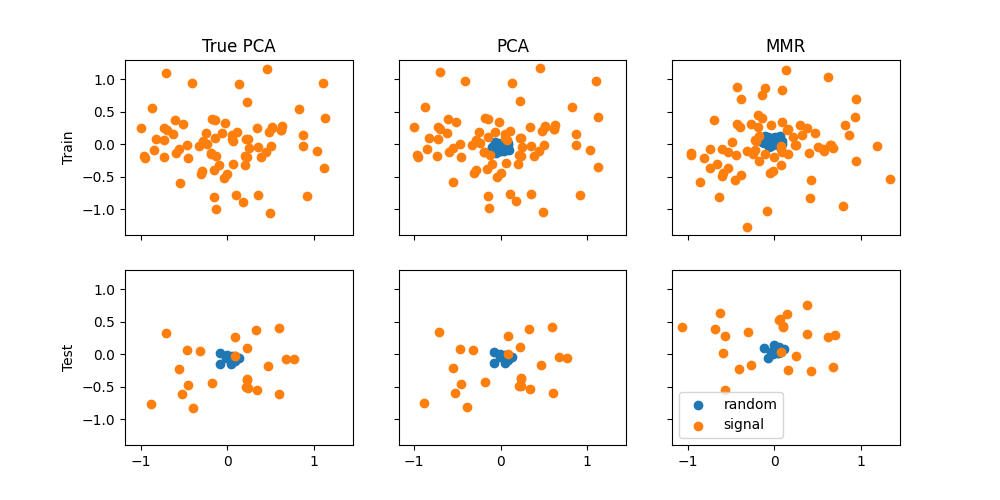
\includegraphics[width=0.9\textwidth]{chapters/sampleselection/pca/models.png}
    \caption{Plots of the first two `principal components' estimated by each model on the x and y axis. The leftmost model is trained using only the interesting data and therefore presents a ground truth}
    \label{fig:pcalatent}
\end{figure}

\begin{figure}[H] 
    \centering
    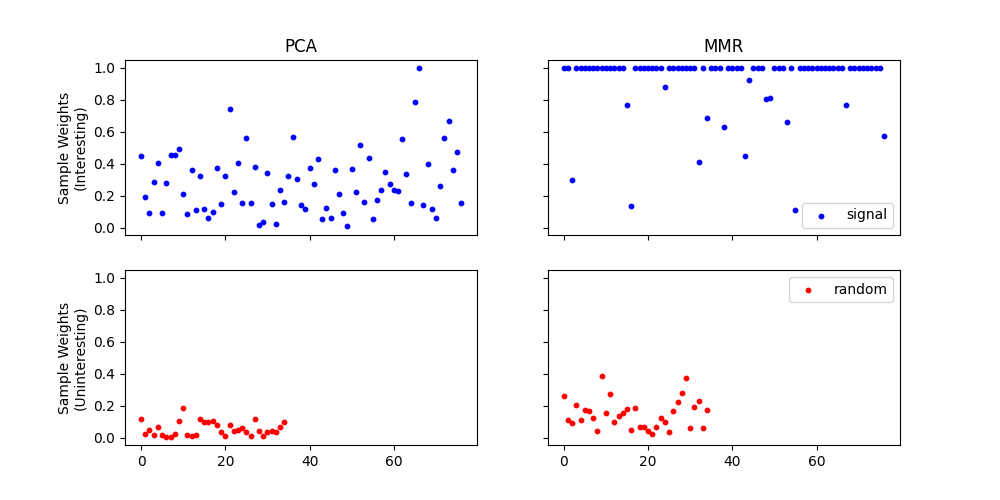
\includegraphics[width=0.9\textwidth]{chapters/sampleselection/pca/weights.png}
    \caption{Plots showing the implied sample weights by both models with the rows separating the interesting samples (top) from the uninteresting samples (bottom). An ideal model would have all samples=1 in the top row and all samples=0 in the bottom.}
    \label{fig:pcaweights}
\end{figure}

\subsection{PLS}

\subsubsection{Experiment Design}

In the PLS experiments, we generate data by combining two multiview datasets. The first is generated using Witten's method described in chapter \ref{chap:framework} while the latter is random noise with the same columnwise variance as the first dataset. We generate 100 interesting samples and 50 uninteresting samples with 10 features in two different views.

One major weakness of using Witten's latent variable model to generate the data with a signal is that the samples associated with the smallest values in the latent variable vector will have lower variance in the data and it is clearly impossible to distinguish between arbitrarily small latent variables and data generated without the latent variables.

We show plots of two views projected onto their first highly covarying latent dimension. We provide a ground truth by running PLS on only the interesting samples. We show projections for both the training data as well as held out test data. The goal for any model is to maximise the covariance of the projections of the `interesting' data.

In addition we show plots of the effective sample weights for each model. Since each model formulates the problem in a slightly different way we highlight that this means:

\begin{itemize}
    \item PLS: The sample wise product of the projections of each view $X_1w_1$ and $X_2w_2$. This is motivated by the fact that samples which drive the covariance objective are those where the projections have the same sign and a large magnitude.
    \item MMR: Since the model uses slack variables to allow for low variance samples, we obtain `sample weights' by subtracting these slack variables from 1. This means a sample with a zero slack variable has sample weight equal to one. A sample with a maximal slack variable equal to one would have a sample weight of zero.
    \item WPLS: The elements of the vector $\bold{d}$ provide a natural sample weighting in their formulation
    
\end{itemize}

\subsubsection{Results}

The results shown in figures \ref{fig:plslatent} and \ref{fig:plsweights} show a degree of promise for using methods which induce sparsity over samples in the PLS context. MMR in particular appears to better suppress the random data when compared to PLS in the latent plots. Interestingly, this is less clear from the sample weighting plots. Our variant of WPLS does not appear to perform well in this context in the sense of successfully recovering the sample weights.

\begin{figure}[H] 
    \centering
    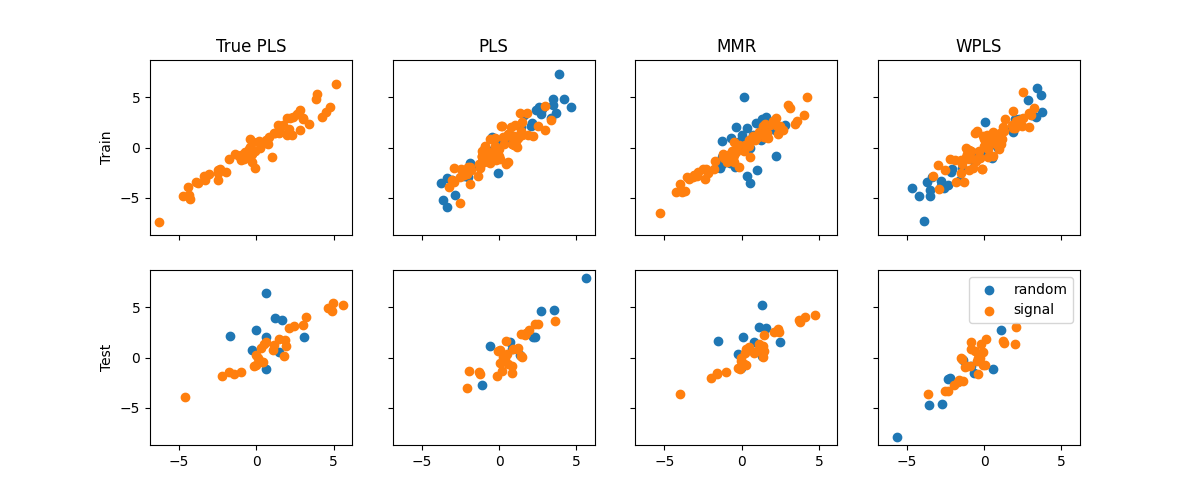
\includegraphics[width=0.9\textwidth]{chapters/sampleselection/pls/models.png}
    \caption{Plots of the first latent score for each view plotted against each other as a scatter plot. The leftmost model is trained using only the interesting data and therefore presents a ground truth}
    \label{fig:plslatent}
\end{figure}

\begin{figure}[H] 
    \centering
    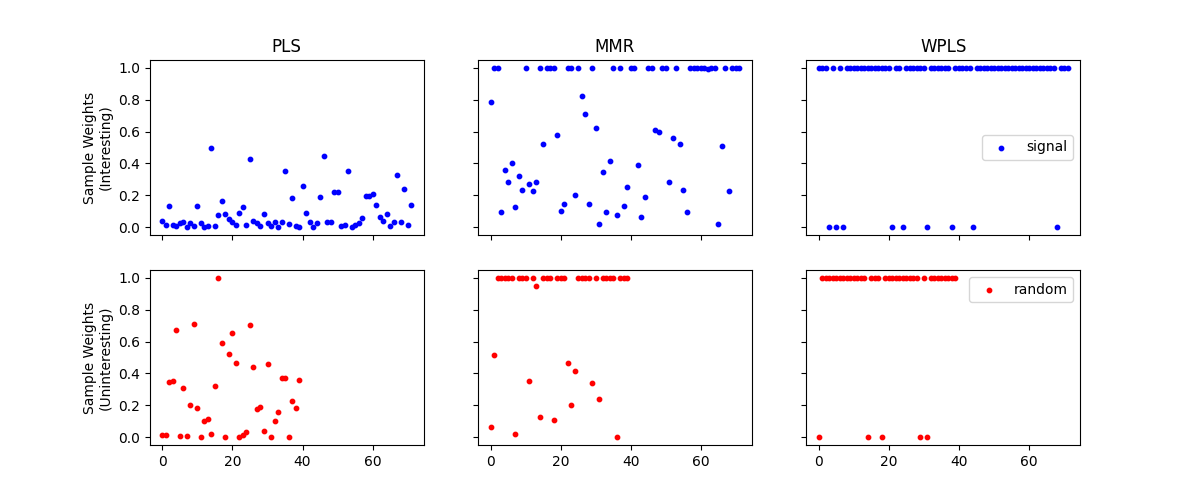
\includegraphics[width=0.9\textwidth]{chapters/sampleselection/pls/weights.png}
    \caption{Plots showing the implied sample weights by both models with the rows separating the interesting samples (top) from the uninteresting samples (bottom). An ideal model would have all samples=1 in the top row and all samples=0 in the bottom.}
    \label{fig:plsweights}
\end{figure}

\subsection{CCA}

\subsubsection{Experiment Design}

In the CCA experiments, data generation follows the same scheme described for the PLS experiments.

We show plots of two views projected onto their first highly correlated latent dimension. We provide a ground truth by running CCA on only the interesting samples. We show projections for both the training data as well as held out test data. The goal for any model is to maximise the correlation of the `interesting data'.

In addition we show plots of the effective sample weights for each model. Since each model formulates the problem in a slightly different way we highlight that this means:

\begin{itemize}
    \item PLS: The sample wise product of the projections of each view $X_1w_1$ and $X_2w_2$. This is motivated by the fact that samples which drive the covariance objective are those where the projections have the same sign and a large magnitude.
    \item MMR: Since the model uses slack variables to allow for low variance samples, we obtain `sample weights' by subtracting these slack variables from 1. This means a sample with a zero slack variable has sample weight equal to one. A sample with a maximal slack variable equal to one would have a sample weight of zero.
    \item WCCA: The elements of the vector $\bold{d}$ provide a natural sample weighting in their formulation
    \item Cluster Correlation: In a binary problem with two groups, we can use the binary classification as a sample weight for visualisation purposes.
\end{itemize}

\subsubsection{Results}

The results shown in figures \ref{fig:ccalatent} and \ref{fig:ccaweights} once again imply some promise for sample selection algorithms. In particular, classical CCA appears to have been driven somewhat by the random data while WCCA and ClusterCorrelation appear to project the interesting samples to a more correlated latent space. The poor performance of MMR suggests a problem with our implementation or construction but is presented for completeness.

\begin{figure}[H] 
    \centering
    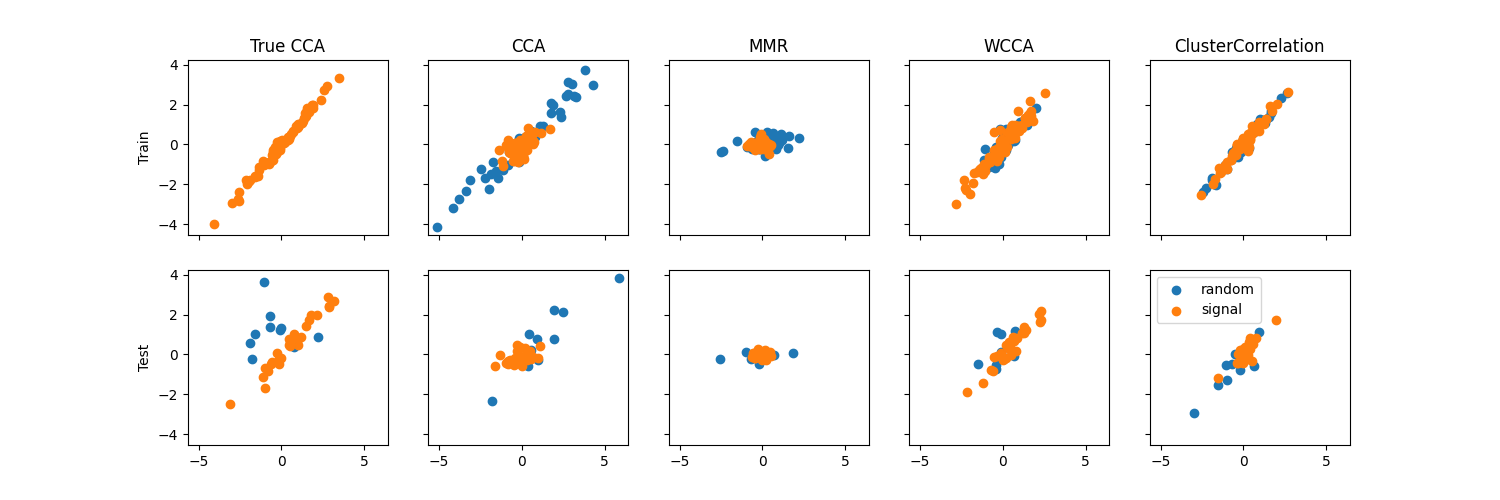
\includegraphics[width=0.9\textwidth]{chapters/sampleselection/cca/models.png}
    \caption{Plots of the first latent score for each view plotted against each other as a scatter plot. The leftmost model is trained using only the interesting data and therefore presents a ground truth}
    \label{fig:ccalatent}
\end{figure}

\begin{figure}[H] 
    \centering
    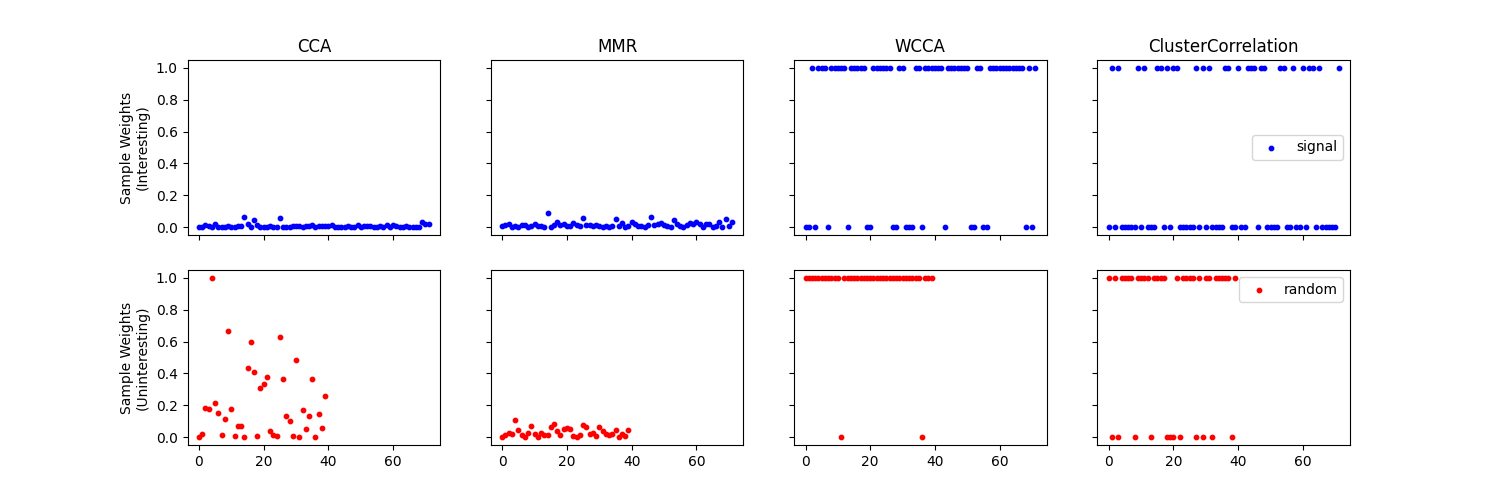
\includegraphics[width=0.9\textwidth]{chapters/sampleselection/cca/weights.png}
    \caption{Plots showing the implied sample weights by both models with the rows separating the interesting samples (top) from the uninteresting samples (bottom). An ideal model would have all samples=1 in the top row and all samples=0 in the bottom.}
    \label{fig:ccaweights}
\end{figure}

\section{Future Work}

This project remains at a somewhat exploratory stage so much of the future work will need to identify situations where these methods could be valuable.

\subsection{Application to GENFI Dataset}

This dataset has the interesting property of containing ground truth subtypes which could be used to validate any promising models. Recent work using Group Factor Analysis \cite{Ferreira2021} has shown promise extracting meaningful brain-behaviour associations using a probabilistic model and upcoming work by the same authors uses probabilistic model with sparsity over subjects. This provides a useful benchmark for our work.



\chapter{Conclusion}

In this thesis, we have motivated the need for developing scalable, flexible, and interpretable multiview SSL methods for biomedical data, especially for population studies of mental health. We have highlighted the challenges and opportunities of working with large-scale and multimodal data sources that can provide diverse and comprehensive information on mental health status and related factors. We had three research questions and objectives that guided our work:

\begin{itemize} 
\item How can we scale classical multiview SSL to the increasingly massive biomedical data available to researchers 
\item How can we incorporate expert priors and interpretability into the models
\item How  can we benefit from the power of deep learning in this space
\end{itemize}

In Chapter 2, we reviewed the existing literature on multiview learning and SSL, and identified the gaps and limitations of the current methods. We also introduced the main concepts and techniques that are relevant for our work, such as subspace learning, regularization, deep neural networks, and stochastic optimization.

In Chapter 3, we reformulated the classical CCA method as an unconstrained optimization problem that can be solved by SGD and therefore scales to large datasets

In Chapter 4, we added regularisation and showed that it improved generalisation (priors) and could be more easily intepreted (sparsity).

In chapter 5 we extended the model to include deep learning functions for learning oomplex highly flexible  functions



\graphicspath{{chapters/software/}}


\chapter{CCA-Zoo: A collection of Regularized, Deep Learning-based, Kernel, and Probabilistic methods in a scikit-learn style framework}\label{ch:software}

% \epigraph{And that's really the essence of programming. By the time you've sorted out a complicated idea into little steps that even a stupid machine can deal with, you've learned something about it yourself.}{\textit{Douglas Adams}}
\minitoc
\section*{Preface}

This work was published in the Journal of Open Source Software \citep{chapman2021cca}.
I have been the lead developer of the \texttt{CCA-Zoo} package since its inception in 2020.
All of the methods we have described in this thesis are implemented in \texttt{CCA-Zoo} and are immediately available for use by the research community.

\section{Introduction}

This chapter presents \texttt{CCA-Zoo}, a comprehensive Python library for multiview learning that was developed as a key contribution of this thesis. \texttt{CCA-Zoo} brings together a wide range of methods for canonical correlation analysis (CCA), partial least squares (PLS), and related techniques, providing efficient and user-friendly implementations that integrate seamlessly with the Python data science ecosystem.

The development of \texttt{CCA-Zoo} was motivated by the recognition that the lack of well-developed and widely available software has been a major barrier to the adoption and advancement of multiview learning methods, particularly in the Python community. While popular libraries like \texttt{scikit-learn} \citep{pedregosa2011scikit} offer basic implementations of classical techniques like CCA and PLS, they lack support for many of the important extensions and variants that have been proposed in the literature to handle challenges such as high-dimensional data, non-linearity, sparsity, and deep learning.

\texttt{CCA-Zoo} aims to fill this gap by providing a unified framework for multiview learning that is both comprehensive and accessible. The library includes implementations of both classical and state-of-the-art methods, ranging from regularized and kernel-based extensions of CCA and PLS to modern deep learning and probabilistic approaches. These implementations are designed to be efficient, scalable, and easy to use, with a consistent API that follows the conventions of \texttt{scikit-learn}.

In addition to its core algorithms, \texttt{CCA-Zoo} provides a range of tools and utilities to support the entire multiview learning workflow, from data preprocessing and feature selection to model evaluation and visualization. The library also includes a collection of example datasets and pre-trained models, making it easy for users to get started and explore different techniques on real-world problems.

Throughout the development of this thesis, \texttt{CCA-Zoo} has played a central role as both a research tool and a means of disseminating our methodological contributions to the wider community. The experiments and case studies presented in the previous chapters have all relied on \texttt{CCA-Zoo} implementations, ensuring reproducibility and comparability of our results. At the same time, by releasing \texttt{CCA-Zoo} as an open-source library on GitHub and PyPi, we have enabled other researchers and practitioners to easily build upon and extend our work.

We also discuss the impact that \texttt{CCA-Zoo} has had so far, both within the context of this thesis and in the broader research community, and outline directions for future development and improvement. Our hope is that \texttt{CCA-Zoo} will serve as a valuable resource and catalyst for advancing the state-of-the-art in multiview learning, and for bridging the gap between methodological research and practical application.

\section{Background: Software for Multiview Learning}

The field of multiview learning has recently witnessed a surge of interest from the research community. This growth can be attributed to the increasing availability of multi-modal data across various domains, from bioinformatics to social media analysis, and the recognition that integrating multiple views can often lead to better insights and predictions than relying on a single perspective.

Traditionally, the development of multiview learning methods has been dominated by researchers in the statistical learning community, who have primarily relied on programming languages like R and MATLAB. These platforms have served as fertile ground for the creation and dissemination of many state-of-the-art algorithms.

However, this has created a challenge for researchers and practitioners who prefer to work in the Python programming language, which has become increasingly popular for machine learning tasks due to its simplicity, flexibility, and rich ecosystem of libraries. Python users have been faced with two suboptimal options: either port existing R or MATLAB implementations into Python, which can be a time-consuming and error-prone process requiring significant domain expertise, or make do with the limited set of multiview methods available in general-purpose Python libraries like \texttt{scikit-learn} \citep{pedregosa2011scikit}.

This fragmentation of the multiview learning landscape across different programming languages has created significant barriers to entry for Python users, potentially hindering the widespread adoption and application of these powerful techniques. Moreover, it has made it difficult for researchers to compare and benchmark different methods on a level playing field, as implementations may vary widely in terms of performance, scalability, and ease of use.

The \texttt{CCA-Zoo} package aims to address these challenges by providing a comprehensive and unified platform for multiview learning in Python. By offering a wide range of algorithms spanning both classical and state-of-the-art approaches, \texttt{CCA-Zoo} enables researchers and practitioners to easily explore and apply these techniques to their own data and problems, without the need for extensive domain expertise or cumbersome porting of code.

Through its scikit-learn compatible API, modular design, and efficient implementations, \texttt{CCA-Zoo} seamlessly integrates with the existing Python machine learning ecosystem, lowering the barriers to entry and accelerating the pace of research and application in multiview learning. By bringing together methods from different research communities and programming languages under a common framework, \texttt{CCA-Zoo} also facilitates fair and reproducible comparisons of different approaches, helping to advance our understanding of their strengths and limitations.

In the following sections, we will consider the design principles, key features, and implementation details of \texttt{CCA-Zoo}, showcasing how it can be used to streamline and enhance multiview learning workflows in Python.

\section{Methods: Design and Implementation of \texttt{CCA-Zoo}}

\texttt{CCA-Zoo} is designed to be a comprehensive and user-friendly library for multiview learning in Python. In this section, we describe the key design decisions and implementation details that underpin its functionality, flexibility, and performance. Figure \ref{fig:cca-zoo-api} provides an overview of the library's structure and its integration with the wider Python machine learning ecosystem.

\subsection{API Design and Scikit-Learn Compatibility}

A central goal in the development of \texttt{CCA-Zoo} was to ensure maximum compatibility and interoperability with the existing Python machine learning ecosystem. To this end, we adopted the API design principles and conventions of the widely-used \texttt{scikit-learn} library \citep{pedregosa2011scikit}. \texttt{Scikit-learn} has become the de facto standard for machine learning in Python, thanks to its consistent, user-friendly API and its extensive collection of tools for data preprocessing, model selection, evaluation, and visualization.

By adhering to the \texttt{scikit-learn} API, \texttt{CCA-Zoo} inherits these benefits and ensures that users can seamlessly integrate multiview learning methods into their existing workflows. All estimators in \texttt{CCA-Zoo} follow the fit-transform pattern, where the \texttt{fit()} method learns model parameters from training data, and the \texttt{transform()} method applies the learned transformation to new data. Hyperparameters are specified as constructor arguments, allowing easy model creation and configuration.

This design choice not only makes \texttt{CCA-Zoo} intuitive and easy to use for anyone familiar with \texttt{scikit-learn}, but also enables the use of \texttt{scikit-learn}'s powerful model selection and evaluation tools, such as cross-validation and grid search, directly with \texttt{CCA-Zoo} estimators. Users can construct complex pipelines that include data preprocessing, feature selection, and multiview learning steps, all with a consistent, declarative syntax.

Figure \ref{fig:cca-zoo-api} illustrates this integration, highlighting \texttt{CCA-Zoo}'s compatibility with key components of the Python machine learning stack.

\begin{figure}[ht]
\centering
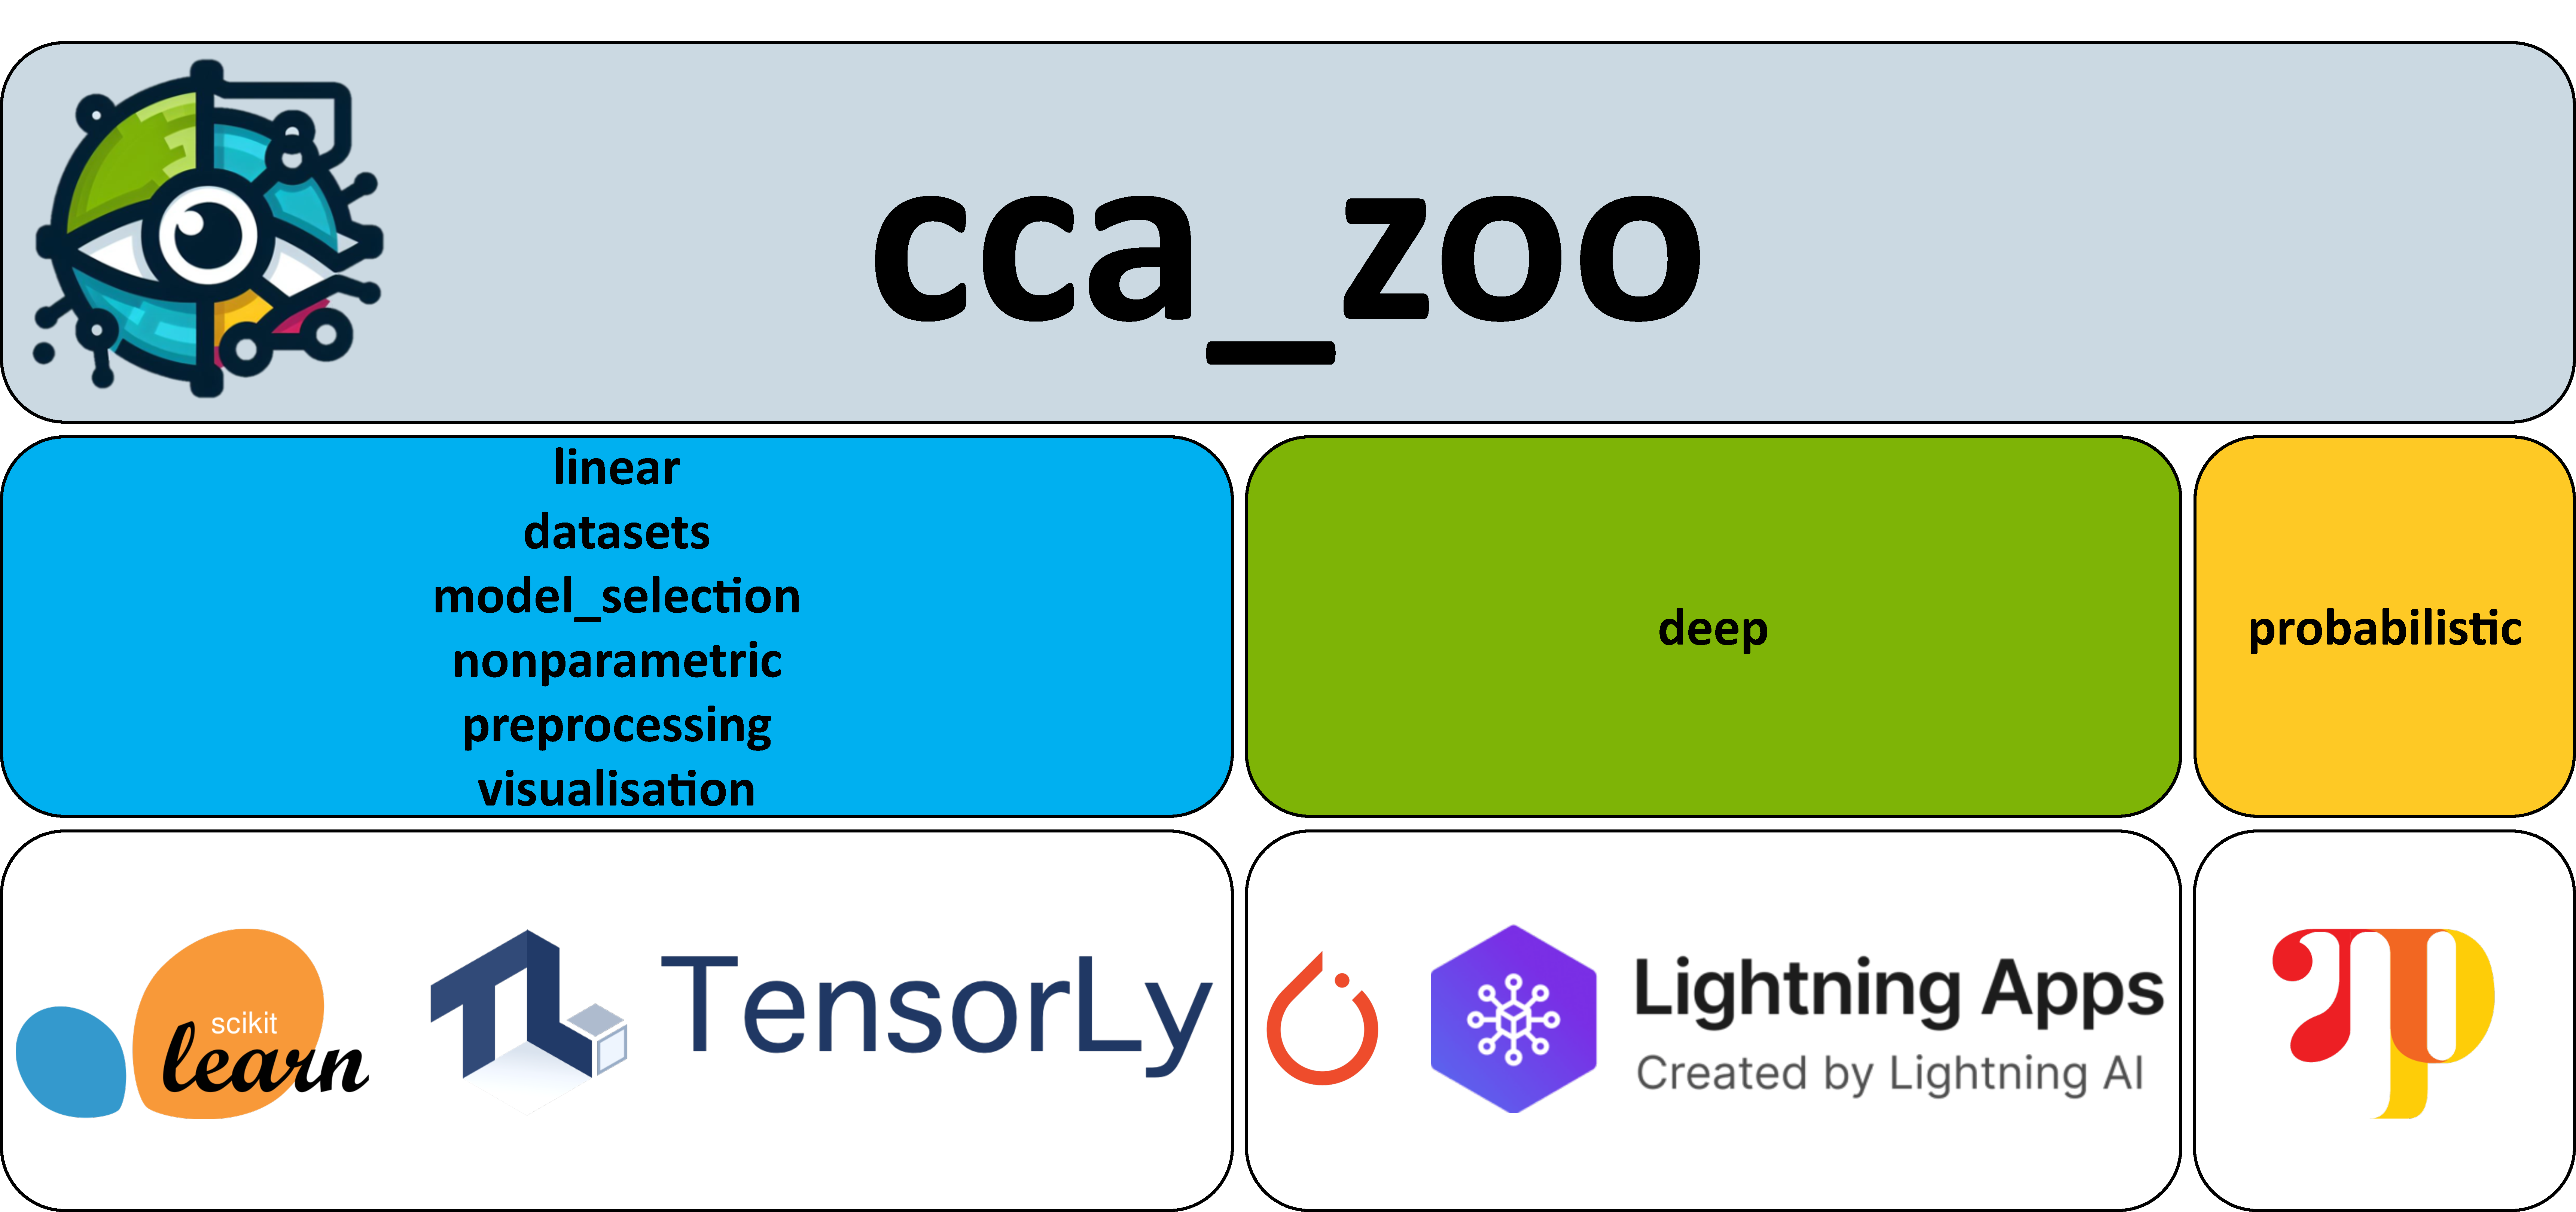
\includegraphics[width=0.8\textwidth]{figures/CCA_Zoo_map}
\caption[The \texttt{CCA-Zoo} compatibility map]{The \texttt{CCA-Zoo} compatibility map showcases integration with various machine learning packages. The deep learning module is built upon \texttt{PyTorch} and \texttt{Lightning}, reflecting their status as industry standards for neural network implementations. The probabilistic module employs \texttt{NumPyro} for its Bayesian inference capabilities, enhancing the application of probabilistic approaches in CCA.}
\label{fig:cca-zoo-api}
\end{figure}

\subsection{Modular Architecture and Extensibility}

Another key design principle of \texttt{CCA-Zoo} is modularity. The library is organized into distinct submodules, each focusing on a specific aspect of the multiview learning workflow:

\begin{itemize}
\item \texttt{datasets}: Classes for generating synthetic data and loading real-world datasets.
\item \texttt{preprocessing}: Tools for data normalization, scaling, and dimensionality reduction.
\item \texttt{model\_selection}: Wrappers for \texttt{scikit-learn}'s cross-validation and hyperparameter tuning utilities, adapted for multiview settings.
\item \texttt{linear}: Estimators for linear CCA, PLS, and their variants.
\item \texttt{deep}: Deep learning-based approaches, built on top of \texttt{PyTorch} \citep{paszke2019pytorch} and \texttt{PyTorch Lightning} \citep{falcon2019pytorch}.
\item \texttt{probabilistic}: Bayesian multiview learning methods, implemented with \texttt{NumPyro} \citep{phan2019composable}, a probabilistic programming library built on top of \texttt{JAX} \citep{deepmind2020jax}.
\item \texttt{visualization}: Functions for visualizing model parameters, latent spaces, and performance metrics.
\end{itemize}

This modular structure makes the codebase more maintainable and easier to navigate. It also facilitates extensibility: new methods and features can be added to each submodule without affecting the rest of the library, as long as they adhere to the common API conventions.

Furthermore, the use of well-established libraries like \texttt{PyTorch}, \texttt{PyTorch Lightning}, and \texttt{NumPyro} for the deep learning and probabilistic modules ensures that \texttt{CCA-Zoo} can benefit from the latest advancements in these rapidly evolving fields. Developers can easily experiment with new architectures, loss functions, and inference techniques, while still leveraging the data handling and model evaluation capabilities of the core \texttt{CCA-Zoo} framework.

\subsection{Flexibility and Ease of Use}

\texttt{CCA-Zoo} is designed to be flexible and easy to use for a wide range of multiview learning tasks. The library provides a unified interface for working with both linear and nonlinear methods, unsupervised and semi-supervised settings, and two-view and multi-view scenarios.

The choice of default hyperparameters and architectural choices for deep learning models has been carefully considered to ensure good performance on a variety of datasets without the need for extensive tuning. At the same time, users have full control over these settings and can easily customize them for specific tasks.

\texttt{CCA-Zoo} also includes a range of utility functions and classes that simplify common tasks and help users avoid boilerplate code. For example, the \texttt{datasets} module provides a consistent interface for accessing and sampling from both synthetic and real-world datasets, handling data loading, splitting, and formatting behind the scenes.

Similarly, the \texttt{model\_selection} module extends \texttt{scikit-learn}'s cross-validation and grid search tools to handle the multi-view setting seamlessly. Users can perform model selection and hyperparameter tuning with just a few lines of code, without having to worry about the intricacies of indexing and reshaping views.

Listing \ref{lst:cca-zoo-example} demonstrates this simplicity and flexibility, showing a complete workflow for training and evaluating a regularized CCA model with cross-validated hyperparameter selection:

% Indent the listing to the right
\begin{listing}[ht]
\begin{minted}{python}
from cca_zoo.datasets import LatentVariableData
from cca_zoo.linear import rCCA
from cca_zoo.model_selection import GridSearchCV
from cca_zoo.visualisation import SeparateRepresentationScatterDisplay

#Generate synthetic multi-view data
data = LatentVariableData(view_features=[10, 10], latent_dims=2)
X, Y = data.sample(n_samples=200, seed=42)

#Define hyperparameter grid
param_grid = {
'c': ([0.1, 0.3, 0.7, 0.9], [0.1, 0.3, 0.7, 0.9]),
}

#Perform cross-validated grid search
model = GridSearchCV(rCCA(latent_dimensions=2),
param_grid=param_grid,
cv=5).fit(X, Y)

#Visualize latent space
SeparateRepresentationScatterDisplay.from_estimator(model.best_estimator_)
\end{minted}
\caption{A complete example of training and evaluating a regularized CCA model with \texttt{CCA-Zoo}.}
\label{lst:cca-zoo-example}
\end{listing}

This example showcases several key features of \texttt{CCA-Zoo}:

\begin{itemize}
\item The \texttt{LatentVariableData} class allows easy generation of synthetic multi-view data with a specified number of features and latent dimensions.
\item The \texttt{rCCA} class provides a regularized CCA estimator with a \texttt{scikit-learn}-compatible API, supporting both fit-transform and inverse transform operations.
\item The \texttt{GridSearchCV} class wraps \texttt{scikit-learn}'s grid search functionality, automatically handling the multi-view parameter grid and cross-validation splitting.
\item The \texttt{SeparateRepresentationScatterDisplay} class provides a high-level interface for visualizing the learned latent space, with separate plots for each view.
\end{itemize}

By providing such high-level abstractions and adhering to familiar API conventions, \texttt{CCA-Zoo} aims to make multiview learning methods accessible to a wide audience, from seasoned machine learning practitioners to domain experts in fields like bioinformatics, computer vision, and natural language processing.

\subsection{Performance and Scalability}

In addition to ease of use and flexibility, \texttt{CCA-Zoo} is designed with performance and scalability in mind. The library is implemented in pure Python, with computationally intensive operations delegated to optimized libraries like \texttt{NumPy} \citep{harris2020array}, \texttt{SciPy} \citep{virtanen2020scipy}, and \texttt{PyTorch}.

For linear methods like CCA and PLS, \texttt{CCA-Zoo} leverages the randomized SVD and other matrix approximation techniques to efficiently handle high-dimensional data. These techniques allow the library to scale to datasets with millions of features and samples, without sacrificing accuracy or numerical stability.

In the deep learning module, \texttt{CCA-Zoo} takes advantage of PyTorch's GPU acceleration and automatic differentiation capabilities to enable fast training of complex models on large-scale datasets. The use of \texttt{PyTorch Lightning} further streamlines the training process, providing a high-level interface for distributed training, checkpointing, and logging.

For probabilistic methods, \texttt{CCA-Zoo} leverages the power of \texttt{NumPyro} and \texttt{JAX} to perform efficient variational inference and MCMC sampling on both CPUs and GPUs. The use of modern probabilistic programming techniques allows users to easily specify and train complex Bayesian models, while still benefiting from the performance and scalability of the underlying libraries.

\texttt{CCA-Zoo}'s performance and scalability claims are backed by extensive benchmarking and testing on a variety of synthetic and real-world datasets. In Section \ref{sec:experiments}, we present a selection of these experiments, comparing \texttt{CCA-Zoo}'s performance to other popular multiview learning libraries and demonstrating its ability to handle large-scale, high-dimensional data.

\subsection{Development and Maintenance}

\texttt{CCA-Zoo} is developed as an open-source project, with its source code and documentation hosted on GitHub at \url{https://github.com/jameschapman19/cca_zoo}. The library follows modern software development best practices, including version control, continuous integration, and automated testing.

The development team is committed to maintaining and improving \texttt{CCA-Zoo} over the long term. This includes fixing bugs, adding new features and methods, and keeping dependencies up to date. The team also welcomes contributions from the community in the form of bug reports, feature requests, and pull requests.

To ensure the library's quality and reliability, \texttt{CCA-Zoo} includes a comprehensive test suite that covers all major functionality. These tests are automatically run on each commit and pull request, using continuous integration services like Travis CI and GitHub Actions. This helps catch regressions and ensures that new features are properly integrated and documented.

\texttt{CCA-Zoo}'s documentation is another key aspect of its maintenance and development. The library includes extensive API documentation, generated automatically from docstrings using tools like Sphinx and Read the Docs. The documentation also includes user guides, tutorials, and examples to help users get started and make the most of the library's features.

In addition to the API documentation, \texttt{CCA-Zoo}'s GitHub repository includes a wiki and issue tracker where users can find additional information, ask questions, and report bugs. The development team is responsive to user feedback and strives to address issues in a timely manner.

By adhering to these development and maintenance practices, \texttt{CCA-Zoo} aims to provide a stable, reliable, and well-documented library that can serve as a foundation for multiview learning research and applications for years to come.

In summary, the key design decisions and implementation details of \texttt{CCA-Zoo} are:

\begin{itemize}
\item Adherence to the \texttt{scikit-learn} API for maximum compatibility and ease of use.
\item Modular architecture for maintainability and extensibility.
\item Flexibility and unified interface for both linear and deep learning methods.
\item Use of optimized libraries and techniques for performance and scalability.
\item Open-source development with modern software engineering practices.
\item Comprehensive documentation and user support.
\end{itemize}

These choices reflect \texttt{CCA-Zoo}'s goal of providing a powerful yet accessible toolkit for multiview learning in Python, suitable for both research and practical applications.

\section{Experiments and Results}\label{sec:experiments}

Throughout this thesis, the \texttt{CCA-Zoo} package has been used extensively for conducting experiments and evaluating the proposed multiview learning methods. The library's comprehensive set of tools and its seamless integration with the Python data science ecosystem have greatly facilitated the implementation and assessment of these methods on a wide range of datasets and tasks.

In this section, we showcase the performance and versatility of \texttt{CCA-Zoo} through a series of benchmarking experiments. These experiments not only demonstrate the efficiency of the library's implementations but also highlight its ability to handle high-dimensional data, a crucial requirement in many real-world applications such as bioinformatics and natural language processing.

\subsection{Benchmarking Setup}

To assess the computational efficiency of \texttt{CCA-Zoo}, we compared its performance against the widely-used \texttt{scikit-learn} library. We focused on two fundamental multiview learning methods: Canonical Correlation Analysis (CCA) and Partial Least Squares (PLS). The experiments were conducted on synthetic datasets of varying dimensionality to evaluate the scalability of the implementations.

The datasets were generated as random matrices with a fixed number of samples (100) and a varying number of features (50, 100, 200, 400, and 800) for each view. The number of latent dimensions was set to 10 for both CCA and PLS. To obtain reliable performance metrics, each experiment was repeated 10 times, and the average execution time was reported.

The benchmarking experiments were performed using the following software versions:

\begin{itemize}
\item \texttt{CCA-Zoo} (version: 2.4.0)
\item \texttt{Scikit-learn} (version: 1.3.0)
\end{itemize}

All experiments were run on a machine with an Intel Core i7-9700K CPU (3.60GHz) and 32GB of RAM, running Ubuntu 20.04.

\subsection{Canonical Correlation Analysis}

Figure~\ref{fig:cca_benchmark} presents the comparison of execution times between \texttt{CCA-Zoo} and \texttt{scikit-learn} for CCA. Across all tested dimensionalities, \texttt{CCA-Zoo} demonstrates competitive performance, with execution times comparable to or better than those of \texttt{scikit-learn}.

\begin{figure}[h]
\centering
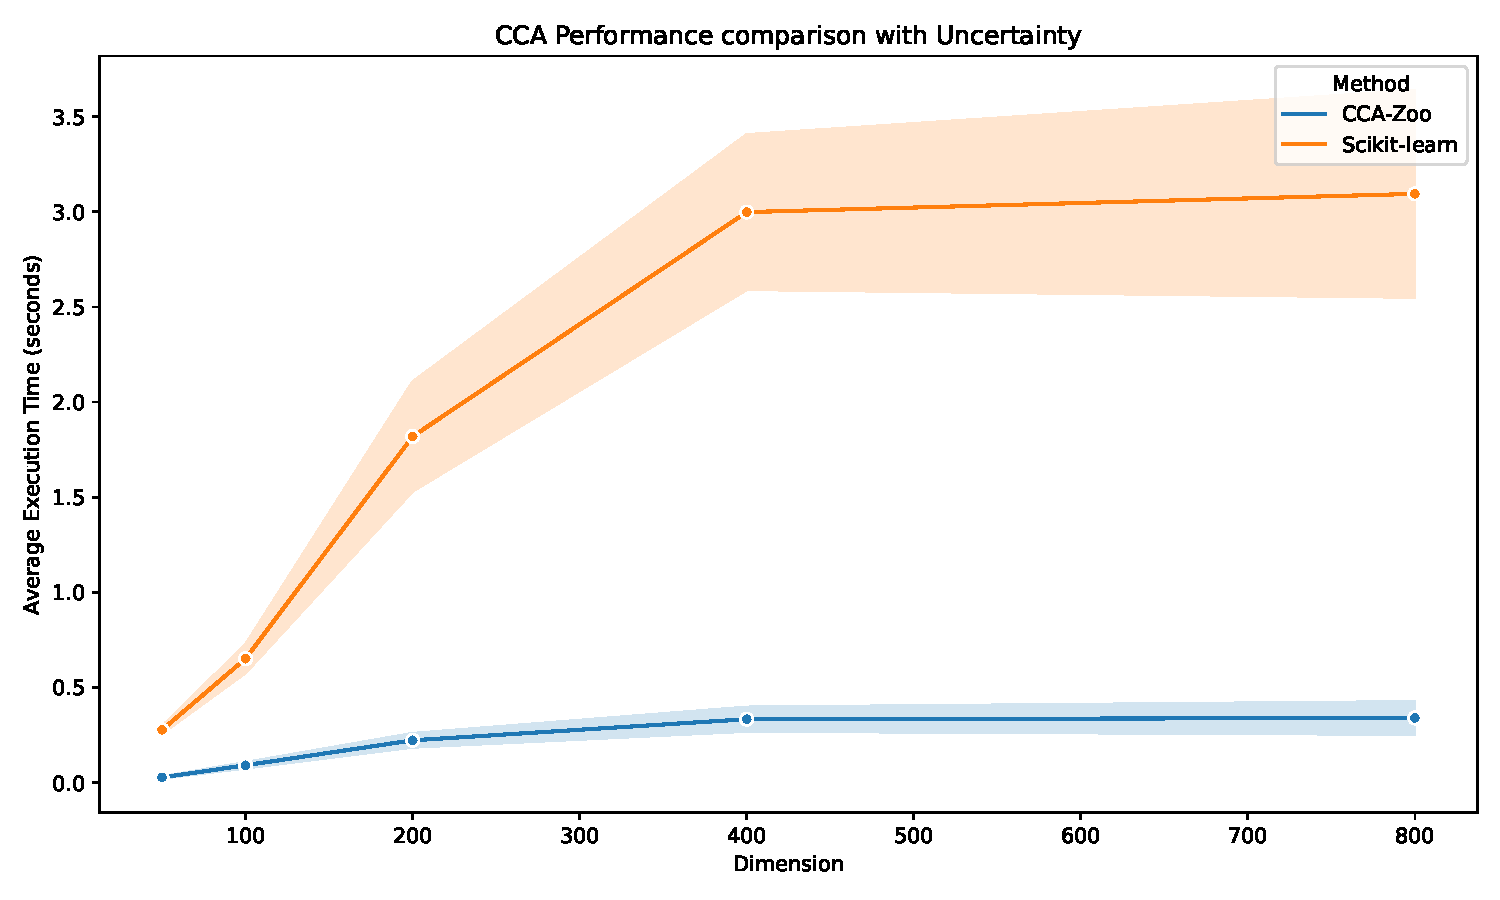
\includegraphics[width=0.9\textwidth]{figures/CCA_Speed_Benchmark}
\caption{Performance comparison for CCA methods}
\label{fig:cca_benchmark}
\end{figure}

The efficiency of \texttt{CCA-Zoo}'s CCA implementation can be attributed to its use of the principal component space for computing the canonical correlations. By first projecting the data onto a lower-dimensional space defined by the leading principal components, \texttt{CCA-Zoo} reduces the computational burden associated with high-dimensional covariance matrices, resulting in faster execution times without sacrificing accuracy.

This performance advantage is particularly relevant in real-world applications, where the number of features often greatly exceeds the number of samples. In such scenarios, \texttt{CCA-Zoo}'s ability to efficiently handle high-dimensional data can lead to significant time savings and enable the analysis of larger datasets.

\subsection{Partial Least Squares}

Figure~\ref{fig:pls_benchmark} shows the execution time comparison for PLS. Similar to the CCA results, \texttt{CCA-Zoo} exhibits a robust performance profile, with execution times that are competitive with those of \texttt{scikit-learn} across all tested dimensionalities.

\begin{figure}[h]
\centering
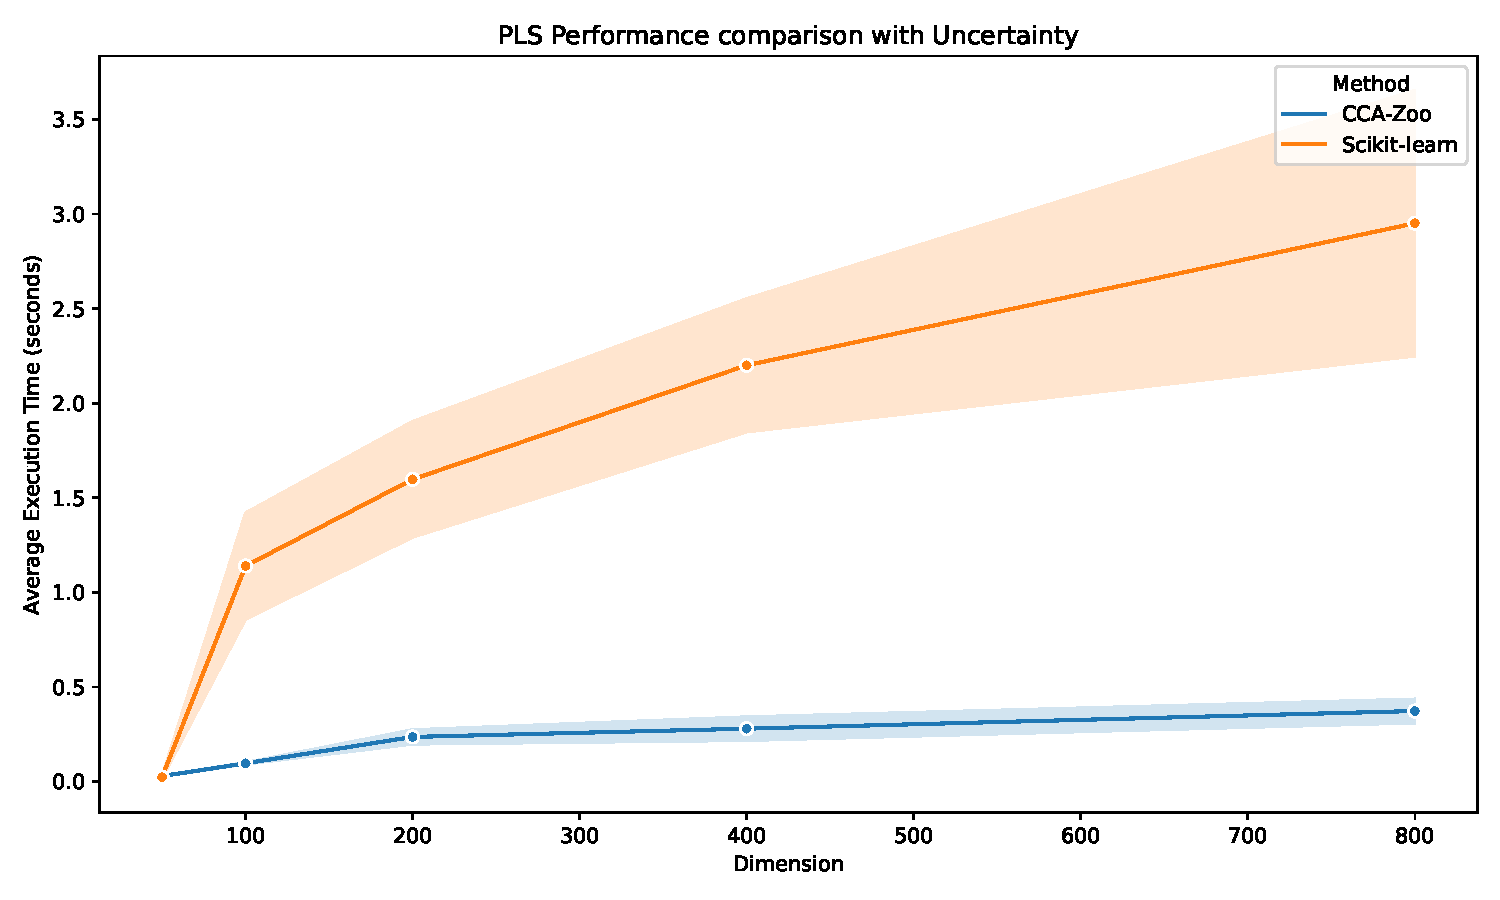
\includegraphics[width=0.9\textwidth]{figures/PLS_Speed_Benchmark}
\caption{Performance comparison for PLS methods}
\label{fig:pls_benchmark}
\end{figure}

The competitive performance of \texttt{CCA-Zoo}'s PLS implementation can be attributed to its use of efficient algorithms and data structures, such as the NIPALS algorithm and the deflation scheme for computing the latent components. These optimizations allow \texttt{CCA-Zoo} to scale well with increasing data dimensionality, making it a suitable choice for a wide range of applications.

\subsection{Real-World Applications}

In addition to the synthetic benchmarking experiments, \texttt{CCA-Zoo} has been used throughout this thesis to evaluate the proposed multiview learning methods on various real-world datasets. These datasets span multiple domains, including bioinformatics and computer vision and pose diverse challenges in terms of dimensionality, sparsity, and noise.

\section{Discussion and Limitations}

\subsection{Contributions and Impact}

The development of \texttt{CCA-Zoo} represents a significant contribution to the field of multiview learning, particularly within the Python ecosystem. By providing a comprehensive and user-friendly library that integrates seamlessly with existing tools like scikit-learn and PyTorch, \texttt{CCA-Zoo} has the potential to greatly accelerate research and application of multiview methods.

Throughout this thesis, \texttt{CCA-Zoo} has played a central role in enabling the empirical studies and method development presented in the previous chapters. The library's efficient implementations of both classical and state-of-the-art multiview algorithms allowed us to conduct extensive experiments on real-world datasets, comparing the performance of different methods and gaining new insights into their behavior. Moreover, the modular design of \texttt{CCA-Zoo} facilitated rapid prototyping and testing of novel extensions and refinements to existing techniques.

Beyond its use in this thesis, \texttt{CCA-Zoo} has already begun to have an impact in the wider research community. The library has been well-received on GitHub, with over 150 stars and 30 forks to date, and has been downloaded nearly 500 times per month from the Python Package Index. Several published papers and ongoing projects in fields ranging from genomics to neuroscience have used CCA-Zoo, demonstrating its potential to enable new discoveries and applications.

\subsection{Limitations and Future Work}

While \texttt{CCA-Zoo} provides a solid foundation for multiview learning in Python, there are certainly areas where it could be improved and extended. One current limitation is the lack of GPU acceleration for some of the more computationally intensive methods, which could hamper their scalability to massive datasets. In future versions, we plan to leverage libraries like cupy to enable seamless GPU support.

Another direction for future work is to expand the library's functionality to encompass an even wider range of multiview learning paradigms, such as multi-modal deep learning, multi-view clustering, and multi-view matrix factorization. By providing a unified interface to these diverse approaches, \texttt{CCA-Zoo} could serve as a powerful toolkit for exploring and combining different perspectives on data.

Finally, we are committed to the ongoing maintenance and development of \texttt{CCA-Zoo} as an open-source project. We welcome contributions from the community in the form of bug reports, feature requests, documentation improvements, and code contributions. By engaging with users and incorporating their feedback, we hope to continuously refine and enhance the library to better serve the needs of multiview learning researchers and practitioners.

\subsection{Conclusion}

In conclusion, \texttt{CCA-Zoo} fills an important gap in the Python ecosystem by providing a comprehensive, efficient, and user-friendly library for multiview learning. Through its extensive catalog of classical and modern multiview methods, seamless integration with popular machine learning tools, and flexible API, \texttt{CCA-Zoo} enables researchers and practitioners to easily explore and apply these powerful techniques to their own data and problems.

The development of \texttt{CCA-Zoo} has been a central contribution of this thesis, underpinning many of the empirical studies and methodological advances presented in earlier chapters. By making the library open-source and freely available to the community, we hope to accelerate progress in multiview learning and promote reproducible, extensible research.

Looking ahead, we see ample opportunities to expand and refine CCA-Zoo, in collaboration with its growing base of users and contributors. Through sustained development and community engagement, we believe \texttt{CCA-Zoo} has the potential to become an indispensable tool in the multiview learning toolkit, enabling new discoveries and applications across a wide range of domains.

% -------------------  BIBLIOGRAPHY ---------------------
\newpage
\addcontentsline{toc}{chapter}{References} % Adds References Section to Table of Contents
\printbibliography[title = {References}]


\end{document}
%  -------------------------------------------------
%  --------- The document ends from here ----------- 
%  -------------------------------------------------